\documentclass[10pt]{report}% ===> this file was generated automatically by noweave --- better not edit it
\usepackage{noweb}
\usepackage{graphicx}

\usepackage[table,dvipsnames]{xcolor}
\definecolor{apple_white}{rgb}{0.9,0.9,0.9}
\def \bk0 {\cellcolor{black}}
\def \bl0 {\cellcolor{Cerulean}}
\def \bw0 {\cellcolor{apple_white}}
\def \bo0 {\cellcolor{orange}}

\usepackage {booktabs}
\usepackage {tikz}
\usetikzlibrary {positioning, shapes.geometric, svg.path}

\noweboptions {smallcode,longchunks}

% Generate assembly file with:
% notangle -Rpreamble main.nw > main.asm
%
% Generate tex file with:
% noweave -delay -index main.nw > main.tex
% pdflatex main.tex (run twice for two passes)
% Indents in code only appears in the PDF output
% under TeX Live 2019.
%
% See also: https://www.cs.tufts.edu/~nr/noweb/johnson-lj.pdf

\begin{document}
\pagestyle{noweb}

\nwfilename{main.nw}\nwbegindocs{1}\chapter{Lode Runner}

\section{Introduction}
For dasm, we'll first specify that we're targeting the 6502 processor:

\nwenddocs{}\nwbegincode{2}\sublabel{NW1Xx3lK-1jwKhK-1}\nwmargintag{{\nwtagstyle{}\subpageref{NW1Xx3lK-1jwKhK-1}}}\moddef{preamble~{\nwtagstyle{}\subpageref{NW1Xx3lK-1jwKhK-1}}}\endmoddef\nwstartdeflinemarkup\nwusesondefline{\\{NW1Xx3lK-1p0Y9w-1}}\nwenddeflinemarkup
    PROCESSOR 6502
\nwused{\\{NW1Xx3lK-1p0Y9w-1}}\nwendcode{}\nwbegindocs{3}That is all!

\chapter{Apple II Graphics}
Hi-res graphics on the Apple II is odd. Graphics are memory-mapped, not exactly
consecutively, and bits don't always correspond to pixels. Color especially is
odd, compared to today's luxurious 32-bit per pixel RGBA.

\section{Pixels and their color}
First we'll talk about pixels. Nominally, the resolution of the hi-res graphics screen
is 280 pixels wide by 192 pixels tall. In the memory map, each row is represented
by 40 bytes. The high bit of each byte is not used for pixel data, but is used to
control color.

Here are some rules for how these bytes are turned into pixels:
\begin{itemize}
  \item Pixels are drawn to the screen from byte data least significant bit first.
        This means that for the first byte bit 0 is column 0, bit 1 is column 1,
        and so on.
  \item A pattern of {\Tt{}11\nwendquote} results in two white pixels at the {\Tt{}1\nwendquote} positions.
  \item A pattern of {\Tt{}010\nwendquote} results at least in a colored pixel at the {\Tt{}1\nwendquote} position.
  \item A pattern of {\Tt{}101\nwendquote} results at least in a colored pixel at the {\Tt{}0\nwendquote} position.
  \item So, a pattern of {\Tt{}01010\nwendquote} results in at least three consecutive colored
        pixels starting from the first {\Tt{}1\nwendquote} to the last {\Tt{}1\nwendquote}. The last {\Tt{}0\nwendquote} bit
        would also be colored if followed by a {\Tt{}1\nwendquote}.
  \item Likewise, a pattern of {\Tt{}11011\nwendquote} results in two white pixels, a colored pixel,
        and then two more white pixels.
  \item The color of a {\Tt{}010\nwendquote} pixel depends on the column that the {\Tt{}1\nwendquote} falls on, and
        also whether the high bit of its byte was set or not. 
  \item The color of a {\Tt{}11011\nwendquote} pixel depends on the column that the {\Tt{}0\nwendquote} falls on, and
        also whether the high bit of its byte was set or not.

        \begin{center}
        \begin{tabular}{@{}rcc@{}} \toprule
        & Odd & Even \\ \cmidrule(r){2-3}
        High bit clear & Green & Violet \\
        High bit set & Orange & Blue \\ \bottomrule
        \end{tabular}
        \end{center}

        The implication is that you can only select one pair of colors per byte.
\end{itemize}

An example would probably be good here. We will take one of the sprites from the game.

\begin{center}
\begin{tabular}{@{}rcc@{}} \toprule
Bytes & Bits & Pixel Data \\ \cmidrule{1-3}
{\Tt{}00\ 00\nwendquote} & {\Tt{}0000000\ 0000000\nwendquote} & {\Tt{}00000000000000\nwendquote} \\
{\Tt{}00\ 00\nwendquote} & {\Tt{}0000000\ 0000000\nwendquote} & {\Tt{}00000000000000\nwendquote} \\
{\Tt{}00\ 00\nwendquote} & {\Tt{}0000000\ 0000000\nwendquote} & {\Tt{}00000000000000\nwendquote} \\
{\Tt{}55\ 00\nwendquote} & {\Tt{}1010101\ 0000000\nwendquote} & {\Tt{}10101010000000\nwendquote} \\
{\Tt{}41\ 00\nwendquote} & {\Tt{}1000001\ 0000000\nwendquote} & {\Tt{}10000010000000\nwendquote} \\
{\Tt{}01\ 00\nwendquote} & {\Tt{}0000001\ 0000000\nwendquote} & {\Tt{}10000000000000\nwendquote} \\
{\Tt{}55\ 00\nwendquote} & {\Tt{}1010101\ 0000000\nwendquote} & {\Tt{}10101010000000\nwendquote} \\
{\Tt{}50\ 00\nwendquote} & {\Tt{}1010000\ 0000000\nwendquote} & {\Tt{}00001010000000\nwendquote} \\
{\Tt{}50\ 00\nwendquote} & {\Tt{}1010000\ 0000000\nwendquote} & {\Tt{}00001010000000\nwendquote} \\
{\Tt{}51\ 00\nwendquote} & {\Tt{}1010001\ 0000000\nwendquote} & {\Tt{}10001010000000\nwendquote} \\
{\Tt{}55\ 00\nwendquote} & {\Tt{}1010101\ 0000000\nwendquote} & {\Tt{}10101010000000\nwendquote} \\ \bottomrule
\end{tabular}
\end{center}

The game automatically sets the high bit of each byte, so we know we're going to see
orange and blue. Assuming that the following bits are all zero, and we place the
sprite starting at column 0, we should see this:

\begin{center}
\begin{tabular}{@{}rcccccccccccccc@{}}
 0 & \bk0 & \bk0 & \bk0 & \bk0 & \bk0 & \bk0 & \bk0 & \bk0 & \bk0 & \bk0 & \bk0 & \bk0 & \bk0 & \bk0 \\
 1 & \bk0 & \bk0 & \bk0 & \bk0 & \bk0 & \bk0 & \bk0 & \bk0 & \bk0 & \bk0 & \bk0 & \bk0 & \bk0 & \bk0 \\
 2 & \bk0 & \bk0 & \bk0 & \bk0 & \bk0 & \bk0 & \bk0 & \bk0 & \bk0 & \bk0 & \bk0 & \bk0 & \bk0 & \bk0 \\
 3 & \bl0 & \bl0 & \bl0 & \bl0 & \bl0 & \bl0 & \bl0 & \bk0 & \bk0 & \bk0 & \bk0 & \bk0 & \bk0 & \bk0 \\
 4 & \bl0 & \bk0 & \bk0 & \bk0 & \bk0 & \bk0 & \bl0 & \bk0 & \bk0 & \bk0 & \bk0 & \bk0 & \bk0 & \bk0 \\
 5 & \bl0 & \bk0 & \bk0 & \bk0 & \bk0 & \bk0 & \bk0 & \bk0 & \bk0 & \bk0 & \bk0 & \bk0 & \bk0 & \bk0 \\
 6 & \bl0 & \bl0 & \bl0 & \bl0 & \bl0 & \bl0 & \bl0 & \bk0 & \bk0 & \bk0 & \bk0 & \bk0 & \bk0 & \bk0 \\
 7 & \bk0 & \bk0 & \bk0 & \bk0 & \bl0 & \bl0 & \bl0 & \bk0 & \bk0 & \bk0 & \bk0 & \bk0 & \bk0 & \bk0 \\
 8 & \bk0 & \bk0 & \bk0 & \bk0 & \bl0 & \bl0 & \bl0 & \bk0 & \bk0 & \bk0 & \bk0 & \bk0 & \bk0 & \bk0 \\
 9 & \bl0 & \bk0 & \bk0 & \bk0 & \bl0 & \bl0 & \bl0 & \bk0 & \bk0 & \bk0 & \bk0 & \bk0 & \bk0 & \bk0 \\
10 & \bl0 & \bl0 & \bl0 & \bl0 & \bl0 & \bl0 & \bl0 & \bk0 & \bk0 & \bk0 & \bk0 & \bk0 & \bk0 & \bk0 \\
\end{tabular}
\end{center}

Here is a more complex sprite:

\begin{center}
\begin{tabular}{@{}rcc@{}} \toprule
Bytes & Bits & Pixel Data \\ \cmidrule{1-3}
{\Tt{}40\ 00\nwendquote} & {\Tt{}1000000\ 0000000\nwendquote} & {\Tt{}00000010000000\nwendquote} \\
{\Tt{}60\ 01\nwendquote} & {\Tt{}1100000\ 0000001\nwendquote} & {\Tt{}00000111000000\nwendquote} \\
{\Tt{}60\ 01\nwendquote} & {\Tt{}1100000\ 0000001\nwendquote} & {\Tt{}00000111000000\nwendquote} \\
{\Tt{}70\ 00\nwendquote} & {\Tt{}1110000\ 0000000\nwendquote} & {\Tt{}00001110000000\nwendquote} \\
{\Tt{}6C\ 01\nwendquote} & {\Tt{}1101100\ 0000001\nwendquote} & {\Tt{}00110111000000\nwendquote} \\
{\Tt{}36\ 06\nwendquote} & {\Tt{}0110110\ 0000110\nwendquote} & {\Tt{}01101100110000\nwendquote} \\
{\Tt{}30\ 00\nwendquote} & {\Tt{}0110000\ 0000000\nwendquote} & {\Tt{}00001100000000\nwendquote} \\
{\Tt{}70\ 00\nwendquote} & {\Tt{}1110000\ 0000000\nwendquote} & {\Tt{}00001110000000\nwendquote} \\
{\Tt{}5E\ 01\nwendquote} & {\Tt{}1011110\ 0000001\nwendquote} & {\Tt{}01111011000000\nwendquote} \\
{\Tt{}40\ 01\nwendquote} & {\Tt{}1000000\ 0000001\nwendquote} & {\Tt{}00000011000000\nwendquote} \\
{\Tt{}40\ 01\nwendquote} & {\Tt{}1000000\ 0000001\nwendquote} & {\Tt{}00000011000000\nwendquote} \\ \bottomrule
\end{tabular}
\end{center}

\begin{center}
\begin{tabular}{@{}rcccccccccccccc@{}}
0 & \bk0 & \bk0 & \bk0 & \bk0 & \bk0 & \bk0 & \bl0 & \bk0 & \bk0 & \bk0 & \bk0 & \bk0 & \bk0 & \bk0 \\
1 & \bk0 & \bk0 & \bk0 & \bk0 & \bk0 & \bw0 & \bw0 & \bw0 & \bk0 & \bk0 & \bk0 & \bk0 & \bk0 & \bk0 \\
2 & \bk0 & \bk0 & \bk0 & \bk0 & \bk0 & \bw0 & \bw0 & \bw0 & \bk0 & \bk0 & \bk0 & \bk0 & \bk0 & \bk0 \\
3 & \bk0 & \bk0 & \bk0 & \bk0 & \bw0 & \bw0 & \bw0 & \bk0 & \bk0 & \bk0 & \bk0 & \bk0 & \bk0 & \bk0 \\
4 & \bk0 & \bk0 & \bw0 & \bw0 & \bo0 & \bw0 & \bw0 & \bw0 & \bk0 & \bk0 & \bk0 & \bk0 & \bk0 & \bk0 \\
5 & \bk0 & \bw0 & \bw0 & \bl0 & \bw0 & \bw0 & \bk0 & \bk0 & \bw0 & \bw0 & \bk0 & \bk0 & \bk0 & \bk0 \\
6 & \bk0 & \bk0 & \bk0 & \bk0 & \bw0 & \bw0 & \bk0 & \bk0 & \bk0 & \bk0 & \bk0 & \bk0 & \bk0 & \bk0 \\
7 & \bk0 & \bk0 & \bk0 & \bk0 & \bw0 & \bw0 & \bw0 & \bk0 & \bk0 & \bk0 & \bk0 & \bk0 & \bk0 & \bk0 \\
8 & \bk0 & \bw0 & \bw0 & \bw0 & \bw0 & \bl0 & \bw0 & \bw0 & \bk0 & \bk0 & \bk0 & \bk0 & \bk0 & \bk0 \\
9 & \bk0 & \bk0 & \bk0 & \bk0 & \bk0 & \bk0 & \bw0 & \bw0 & \bk0 & \bk0 & \bk0 & \bk0 & \bk0 & \bk0 \\
10 & \bk0 & \bk0 & \bk0 & \bk0 & \bk0 & \bk0 & \bw0 & \bw0 & \bk0 & \bk0 & \bk0 & \bk0 & \bk0 & \bk0 \\
\end{tabular}
\end{center}

Take note of the orange and blue pixels. All the patterns noted in the rules above are used.

\section{The sprites}
Lode Runner defines 104 sprites, each being 11 rows, with two bytes per row. The first bytes of
all 104 sprites are in the table first, then the second bytes, then the third bytes, and so on.

\begin{center}
\scalebox{0.8}{
\begin{tabular}{@{}rcccccccccccccccccccccccccccccc@{}}
 & \multicolumn{14}{c}{Sprite 0} & & \multicolumn{14}{c}{Sprite 1} \\
0 & \bk0 & \bk0 & \bk0 & \bk0 & \bk0 & \bk0 & \bk0 & \bk0 & \bk0 & \bk0 & \bk0 & \bk0 & \bk0 & \bk0 & & \bl0 & \bl0 & \bl0 & \bl0 & \bl0 & \bk0 & \bk0 & \bk0 & \bl0 & \bk0 & \bk0 & \bk0 & \bk0 & \bk0 & \\
1 & \bk0 & \bk0 & \bk0 & \bk0 & \bk0 & \bk0 & \bk0 & \bk0 & \bk0 & \bk0 & \bk0 & \bk0 & \bk0 & \bk0 & & \bl0 & \bl0 & \bl0 & \bl0 & \bl0 & \bk0 & \bk0 & \bk0 & \bl0 & \bk0 & \bk0 & \bk0 & \bk0 & \bk0 & \\
2 & \bk0 & \bk0 & \bk0 & \bk0 & \bk0 & \bk0 & \bk0 & \bk0 & \bk0 & \bk0 & \bk0 & \bk0 & \bk0 & \bk0 & & \bl0 & \bl0 & \bl0 & \bl0 & \bl0 & \bk0 & \bk0 & \bk0 & \bl0 & \bk0 & \bk0 & \bk0 & \bk0 & \bk0 & \\
3 & \bk0 & \bk0 & \bk0 & \bk0 & \bk0 & \bk0 & \bk0 & \bk0 & \bk0 & \bk0 & \bk0 & \bk0 & \bk0 & \bk0 & & \bl0 & \bl0 & \bl0 & \bl0 & \bl0 & \bk0 & \bk0 & \bk0 & \bl0 & \bk0 & \bk0 & \bk0 & \bk0 & \bk0 & \\
4 & \bk0 & \bk0 & \bk0 & \bk0 & \bk0 & \bk0 & \bk0 & \bk0 & \bk0 & \bk0 & \bk0 & \bk0 & \bk0 & \bk0 & & \bk0 & \bk0 & \bk0 & \bk0 & \bk0 & \bk0 & \bk0 & \bk0 & \bk0 & \bk0 & \bk0 & \bk0 & \bk0 & \bk0 & \\
5 & \bk0 & \bk0 & \bk0 & \bk0 & \bk0 & \bk0 & \bk0 & \bk0 & \bk0 & \bk0 & \bk0 & \bk0 & \bk0 & \bk0 & & \bl0 & \bk0 & \bk0 & \bk0 & \bl0 & \bl0 & \bl0 & \bl0 & \bl0 & \bk0 & \bk0 & \bk0 & \bk0 & \bk0 & \\
6 & \bk0 & \bk0 & \bk0 & \bk0 & \bk0 & \bk0 & \bk0 & \bk0 & \bk0 & \bk0 & \bk0 & \bk0 & \bk0 & \bk0 & & \bl0 & \bk0 & \bk0 & \bk0 & \bl0 & \bl0 & \bl0 & \bl0 & \bl0 & \bk0 & \bk0 & \bk0 & \bk0 & \bk0 & \\
7 & \bk0 & \bk0 & \bk0 & \bk0 & \bk0 & \bk0 & \bk0 & \bk0 & \bk0 & \bk0 & \bk0 & \bk0 & \bk0 & \bk0 & & \bl0 & \bk0 & \bk0 & \bk0 & \bl0 & \bl0 & \bl0 & \bl0 & \bl0 & \bk0 & \bk0 & \bk0 & \bk0 & \bk0 & \\
8 & \bk0 & \bk0 & \bk0 & \bk0 & \bk0 & \bk0 & \bk0 & \bk0 & \bk0 & \bk0 & \bk0 & \bk0 & \bk0 & \bk0 & & \bl0 & \bk0 & \bk0 & \bk0 & \bl0 & \bl0 & \bl0 & \bl0 & \bl0 & \bk0 & \bk0 & \bk0 & \bk0 & \bk0 & \\
9 & \bk0 & \bk0 & \bk0 & \bk0 & \bk0 & \bk0 & \bk0 & \bk0 & \bk0 & \bk0 & \bk0 & \bk0 & \bk0 & \bk0 & & \bl0 & \bk0 & \bk0 & \bk0 & \bl0 & \bl0 & \bl0 & \bl0 & \bl0 & \bk0 & \bk0 & \bk0 & \bk0 & \bk0 & \\
10 & \bk0 & \bk0 & \bk0 & \bk0 & \bk0 & \bk0 & \bk0 & \bk0 & \bk0 & \bk0 & \bk0 & \bk0 & \bk0 & \bk0 & & \bk0 & \bk0 & \bk0 & \bk0 & \bk0 & \bk0 & \bk0 & \bk0 & \bk0 & \bk0 & \bk0 & \bk0 & \bk0 & \bk0 & \\
\end{tabular}
}
\end{center}
\begin{center}
\scalebox{0.8}{
\begin{tabular}{@{}rcccccccccccccccccccccccccccccc@{}}
 & \multicolumn{14}{c}{Sprite 2} & & \multicolumn{14}{c}{Sprite 3} \\
0 & \bl0 & \bl0 & \bl0 & \bl0 & \bl0 & \bl0 & \bl0 & \bl0 & \bl0 & \bk0 & \bk0 & \bk0 & \bk0 & \bk0 & & \bk0 & \bw0 & \bw0 & \bk0 & \bk0 & \bk0 & \bk0 & \bw0 & \bw0 & \bk0 & \bk0 & \bk0 & \bk0 & \bk0 & \\
1 & \bl0 & \bl0 & \bl0 & \bl0 & \bl0 & \bl0 & \bl0 & \bl0 & \bl0 & \bk0 & \bk0 & \bk0 & \bk0 & \bk0 & & \bk0 & \bw0 & \bw0 & \bk0 & \bk0 & \bk0 & \bk0 & \bw0 & \bw0 & \bk0 & \bk0 & \bk0 & \bk0 & \bk0 & \\
2 & \bl0 & \bl0 & \bl0 & \bl0 & \bl0 & \bl0 & \bl0 & \bl0 & \bl0 & \bk0 & \bk0 & \bk0 & \bk0 & \bk0 & & \bk0 & \bw0 & \bw0 & \bw0 & \bw0 & \bw0 & \bw0 & \bw0 & \bw0 & \bk0 & \bk0 & \bk0 & \bk0 & \bk0 & \\
3 & \bl0 & \bl0 & \bl0 & \bl0 & \bl0 & \bl0 & \bl0 & \bl0 & \bl0 & \bk0 & \bk0 & \bk0 & \bk0 & \bk0 & & \bk0 & \bw0 & \bw0 & \bk0 & \bk0 & \bk0 & \bk0 & \bw0 & \bw0 & \bk0 & \bk0 & \bk0 & \bk0 & \bk0 & \\
4 & \bl0 & \bl0 & \bl0 & \bl0 & \bl0 & \bl0 & \bl0 & \bl0 & \bl0 & \bk0 & \bk0 & \bk0 & \bk0 & \bk0 & & \bk0 & \bw0 & \bw0 & \bk0 & \bk0 & \bk0 & \bk0 & \bw0 & \bw0 & \bk0 & \bk0 & \bk0 & \bk0 & \bk0 & \\
5 & \bl0 & \bl0 & \bl0 & \bl0 & \bl0 & \bl0 & \bl0 & \bl0 & \bl0 & \bk0 & \bk0 & \bk0 & \bk0 & \bk0 & & \bk0 & \bw0 & \bw0 & \bk0 & \bk0 & \bk0 & \bk0 & \bw0 & \bw0 & \bk0 & \bk0 & \bk0 & \bk0 & \bk0 & \\
6 & \bl0 & \bl0 & \bl0 & \bl0 & \bl0 & \bl0 & \bl0 & \bl0 & \bl0 & \bk0 & \bk0 & \bk0 & \bk0 & \bk0 & & \bk0 & \bw0 & \bw0 & \bk0 & \bk0 & \bk0 & \bk0 & \bw0 & \bw0 & \bk0 & \bk0 & \bk0 & \bk0 & \bk0 & \\
7 & \bl0 & \bl0 & \bl0 & \bl0 & \bl0 & \bl0 & \bl0 & \bl0 & \bl0 & \bk0 & \bk0 & \bk0 & \bk0 & \bk0 & & \bk0 & \bw0 & \bw0 & \bw0 & \bw0 & \bw0 & \bw0 & \bw0 & \bw0 & \bk0 & \bk0 & \bk0 & \bk0 & \bk0 & \\
8 & \bl0 & \bl0 & \bl0 & \bl0 & \bl0 & \bl0 & \bl0 & \bl0 & \bl0 & \bk0 & \bk0 & \bk0 & \bk0 & \bk0 & & \bk0 & \bw0 & \bw0 & \bk0 & \bk0 & \bk0 & \bk0 & \bw0 & \bw0 & \bk0 & \bk0 & \bk0 & \bk0 & \bk0 & \\
9 & \bl0 & \bl0 & \bl0 & \bl0 & \bl0 & \bl0 & \bl0 & \bl0 & \bl0 & \bk0 & \bk0 & \bk0 & \bk0 & \bk0 & & \bk0 & \bw0 & \bw0 & \bk0 & \bk0 & \bk0 & \bk0 & \bw0 & \bw0 & \bk0 & \bk0 & \bk0 & \bk0 & \bk0 & \\
10 & \bk0 & \bk0 & \bk0 & \bk0 & \bk0 & \bk0 & \bk0 & \bk0 & \bk0 & \bk0 & \bk0 & \bk0 & \bk0 & \bk0 & & \bk0 & \bw0 & \bw0 & \bk0 & \bk0 & \bk0 & \bk0 & \bw0 & \bw0 & \bk0 & \bk0 & \bk0 & \bk0 & \bk0 & \\
\end{tabular}
}
\end{center}
\begin{center}
\scalebox{0.8}{
\begin{tabular}{@{}rcccccccccccccccccccccccccccccc@{}}
 & \multicolumn{14}{c}{Sprite 4} & & \multicolumn{14}{c}{Sprite 5} \\
0 & \bk0 & \bk0 & \bk0 & \bk0 & \bk0 & \bk0 & \bk0 & \bk0 & \bk0 & \bk0 & \bk0 & \bk0 & \bk0 & \bk0 & & \bl0 & \bl0 & \bl0 & \bl0 & \bl0 & \bl0 & \bl0 & \bl0 & \bl0 & \bk0 & \bk0 & \bk0 & \bk0 & \bk0 & \\
1 & \bw0 & \bw0 & \bw0 & \bw0 & \bw0 & \bw0 & \bw0 & \bw0 & \bw0 & \bw0 & \bk0 & \bk0 & \bk0 & \bk0 & & \bl0 & \bl0 & \bl0 & \bl0 & \bl0 & \bl0 & \bl0 & \bl0 & \bl0 & \bk0 & \bk0 & \bk0 & \bk0 & \bk0 & \\
2 & \bk0 & \bk0 & \bk0 & \bk0 & \bk0 & \bk0 & \bk0 & \bk0 & \bk0 & \bk0 & \bk0 & \bk0 & \bk0 & \bk0 & & \bk0 & \bk0 & \bk0 & \bk0 & \bk0 & \bk0 & \bk0 & \bk0 & \bk0 & \bk0 & \bk0 & \bk0 & \bk0 & \bk0 & \\
3 & \bk0 & \bk0 & \bk0 & \bk0 & \bk0 & \bk0 & \bk0 & \bk0 & \bk0 & \bk0 & \bk0 & \bk0 & \bk0 & \bk0 & & \bk0 & \bk0 & \bw0 & \bw0 & \bw0 & \bw0 & \bw0 & \bw0 & \bk0 & \bk0 & \bk0 & \bk0 & \bk0 & \bk0 & \\
4 & \bk0 & \bk0 & \bk0 & \bk0 & \bk0 & \bk0 & \bk0 & \bk0 & \bk0 & \bk0 & \bk0 & \bk0 & \bk0 & \bk0 & & \bk0 & \bk0 & \bk0 & \bk0 & \bw0 & \bw0 & \bk0 & \bk0 & \bk0 & \bk0 & \bk0 & \bk0 & \bk0 & \bk0 & \\
5 & \bk0 & \bk0 & \bk0 & \bk0 & \bk0 & \bk0 & \bk0 & \bk0 & \bk0 & \bk0 & \bk0 & \bk0 & \bk0 & \bk0 & & \bk0 & \bk0 & \bk0 & \bk0 & \bw0 & \bw0 & \bk0 & \bk0 & \bk0 & \bk0 & \bk0 & \bk0 & \bk0 & \bk0 & \\
6 & \bk0 & \bk0 & \bk0 & \bk0 & \bk0 & \bk0 & \bk0 & \bk0 & \bk0 & \bk0 & \bk0 & \bk0 & \bk0 & \bk0 & & \bk0 & \bk0 & \bk0 & \bk0 & \bw0 & \bw0 & \bk0 & \bk0 & \bk0 & \bk0 & \bk0 & \bk0 & \bk0 & \bk0 & \\
7 & \bk0 & \bk0 & \bk0 & \bk0 & \bk0 & \bk0 & \bk0 & \bk0 & \bk0 & \bk0 & \bk0 & \bk0 & \bk0 & \bk0 & & \bk0 & \bk0 & \bk0 & \bk0 & \bw0 & \bw0 & \bk0 & \bk0 & \bk0 & \bk0 & \bk0 & \bk0 & \bk0 & \bk0 & \\
8 & \bk0 & \bk0 & \bk0 & \bk0 & \bk0 & \bk0 & \bk0 & \bk0 & \bk0 & \bk0 & \bk0 & \bk0 & \bk0 & \bk0 & & \bl0 & \bl0 & \bl0 & \bl0 & \bl0 & \bl0 & \bl0 & \bl0 & \bl0 & \bk0 & \bk0 & \bk0 & \bk0 & \bk0 & \\
9 & \bk0 & \bk0 & \bk0 & \bk0 & \bk0 & \bk0 & \bk0 & \bk0 & \bk0 & \bk0 & \bk0 & \bk0 & \bk0 & \bk0 & & \bl0 & \bl0 & \bl0 & \bl0 & \bl0 & \bl0 & \bl0 & \bl0 & \bl0 & \bk0 & \bk0 & \bk0 & \bk0 & \bk0 & \\
10 & \bk0 & \bk0 & \bk0 & \bk0 & \bk0 & \bk0 & \bk0 & \bk0 & \bk0 & \bk0 & \bk0 & \bk0 & \bk0 & \bk0 & & \bk0 & \bk0 & \bk0 & \bk0 & \bk0 & \bk0 & \bk0 & \bk0 & \bk0 & \bk0 & \bk0 & \bk0 & \bk0 & \bk0 & \\
\end{tabular}
}
\end{center}
\begin{center}
\scalebox{0.8}{
\begin{tabular}{@{}rcccccccccccccccccccccccccccccc@{}}
 & \multicolumn{14}{c}{Sprite 6} & & \multicolumn{14}{c}{Sprite 7} \\
0 & \bk0 & \bw0 & \bw0 & \bk0 & \bk0 & \bk0 & \bk0 & \bk0 & \bk0 & \bk0 & \bk0 & \bk0 & \bk0 & \bk0 & & \bk0 & \bk0 & \bk0 & \bk0 & \bk0 & \bk0 & \bk0 & \bk0 & \bk0 & \bk0 & \bk0 & \bk0 & \bk0 & \bk0 & \\
1 & \bk0 & \bw0 & \bw0 & \bk0 & \bk0 & \bk0 & \bk0 & \bk0 & \bk0 & \bk0 & \bk0 & \bk0 & \bk0 & \bk0 & & \bk0 & \bk0 & \bk0 & \bk0 & \bk0 & \bk0 & \bk0 & \bk0 & \bk0 & \bk0 & \bk0 & \bk0 & \bk0 & \bk0 & \\
2 & \bk0 & \bw0 & \bw0 & \bw0 & \bw0 & \bw0 & \bw0 & \bw0 & \bw0 & \bk0 & \bk0 & \bk0 & \bk0 & \bk0 & & \bk0 & \bk0 & \bk0 & \bk0 & \bk0 & \bk0 & \bk0 & \bk0 & \bk0 & \bk0 & \bk0 & \bk0 & \bk0 & \bk0 & \\
3 & \bk0 & \bw0 & \bw0 & \bk0 & \bk0 & \bk0 & \bk0 & \bw0 & \bw0 & \bk0 & \bk0 & \bk0 & \bk0 & \bk0 & & \bk0 & \bk0 & \bk0 & \bk0 & \bk0 & \bk0 & \bk0 & \bk0 & \bk0 & \bk0 & \bk0 & \bk0 & \bk0 & \bk0 & \\
4 & \bk0 & \bk0 & \bk0 & \bk0 & \bk0 & \bk0 & \bk0 & \bw0 & \bw0 & \bk0 & \bk0 & \bk0 & \bk0 & \bk0 & & \bk0 & \bk0 & \bk0 & \bk0 & \bk0 & \bk0 & \bk0 & \bk0 & \bk0 & \bk0 & \bk0 & \bk0 & \bk0 & \bk0 & \\
5 & \bk0 & \bk0 & \bk0 & \bk0 & \bk0 & \bk0 & \bk0 & \bw0 & \bw0 & \bk0 & \bk0 & \bk0 & \bk0 & \bk0 & & \bk0 & \bk0 & \bk0 & \bw0 & \bw0 & \bw0 & \bw0 & \bw0 & \bk0 & \bk0 & \bk0 & \bk0 & \bk0 & \bk0 & \\
6 & \bk0 & \bk0 & \bk0 & \bk0 & \bk0 & \bk0 & \bk0 & \bw0 & \bw0 & \bk0 & \bk0 & \bk0 & \bk0 & \bk0 & & \bk0 & \bk0 & \bk0 & \bo0 & \bo0 & \bo0 & \bo0 & \bo0 & \bk0 & \bk0 & \bk0 & \bk0 & \bk0 & \bk0 & \\
7 & \bk0 & \bw0 & \bw0 & \bk0 & \bk0 & \bk0 & \bk0 & \bw0 & \bw0 & \bk0 & \bk0 & \bk0 & \bk0 & \bk0 & & \bk0 & \bk0 & \bk0 & \bw0 & \bw0 & \bw0 & \bw0 & \bw0 & \bk0 & \bk0 & \bk0 & \bk0 & \bk0 & \bk0 & \\
8 & \bk0 & \bw0 & \bw0 & \bw0 & \bw0 & \bw0 & \bw0 & \bw0 & \bw0 & \bk0 & \bk0 & \bk0 & \bk0 & \bk0 & & \bk0 & \bk0 & \bk0 & \bo0 & \bo0 & \bo0 & \bo0 & \bo0 & \bk0 & \bk0 & \bk0 & \bk0 & \bk0 & \bk0 & \\
9 & \bk0 & \bw0 & \bw0 & \bk0 & \bk0 & \bk0 & \bk0 & \bk0 & \bk0 & \bk0 & \bk0 & \bk0 & \bk0 & \bk0 & & \bk0 & \bk0 & \bk0 & \bw0 & \bw0 & \bw0 & \bw0 & \bw0 & \bk0 & \bk0 & \bk0 & \bk0 & \bk0 & \bk0 & \\
10 & \bk0 & \bw0 & \bw0 & \bk0 & \bk0 & \bk0 & \bk0 & \bk0 & \bk0 & \bk0 & \bk0 & \bk0 & \bk0 & \bk0 & & \bk0 & \bk0 & \bk0 & \bk0 & \bk0 & \bk0 & \bk0 & \bk0 & \bk0 & \bk0 & \bk0 & \bk0 & \bk0 & \bk0 & \\
\end{tabular}
}
\end{center}
\begin{center}
\scalebox{0.8}{
\begin{tabular}{@{}rcccccccccccccccccccccccccccccc@{}}
 & \multicolumn{14}{c}{Sprite 8} & & \multicolumn{14}{c}{Sprite 9} \\
0 & \bk0 & \bk0 & \bk0 & \bk0 & \bl0 & \bk0 & \bk0 & \bk0 & \bk0 & \bk0 & \bk0 & \bk0 & \bk0 & \bk0 & & \bk0 & \bk0 & \bk0 & \bk0 & \bk0 & \bk0 & \bl0 & \bk0 & \bk0 & \bk0 & \bk0 & \bk0 & \bk0 & \bk0 & \\
1 & \bk0 & \bk0 & \bk0 & \bo0 & \bo0 & \bo0 & \bk0 & \bk0 & \bk0 & \bk0 & \bk0 & \bk0 & \bk0 & \bk0 & & \bk0 & \bk0 & \bk0 & \bk0 & \bk0 & \bw0 & \bw0 & \bw0 & \bk0 & \bk0 & \bk0 & \bk0 & \bk0 & \bk0 & \\
2 & \bk0 & \bk0 & \bk0 & \bo0 & \bo0 & \bo0 & \bk0 & \bk0 & \bk0 & \bk0 & \bk0 & \bk0 & \bk0 & \bk0 & & \bk0 & \bk0 & \bk0 & \bk0 & \bk0 & \bw0 & \bw0 & \bw0 & \bk0 & \bk0 & \bk0 & \bk0 & \bk0 & \bk0 & \\
3 & \bk0 & \bk0 & \bk0 & \bk0 & \bk0 & \bo0 & \bk0 & \bk0 & \bk0 & \bk0 & \bk0 & \bk0 & \bk0 & \bk0 & & \bk0 & \bk0 & \bk0 & \bk0 & \bw0 & \bw0 & \bw0 & \bk0 & \bk0 & \bk0 & \bk0 & \bk0 & \bk0 & \bk0 & \\
4 & \bk0 & \bk0 & \bk0 & \bo0 & \bo0 & \bo0 & \bo0 & \bo0 & \bk0 & \bk0 & \bk0 & \bk0 & \bk0 & \bk0 & & \bk0 & \bk0 & \bw0 & \bw0 & \bo0 & \bw0 & \bw0 & \bw0 & \bk0 & \bk0 & \bk0 & \bk0 & \bk0 & \bk0 & \\
5 & \bk0 & \bo0 & \bk0 & \bk0 & \bk0 & \bo0 & \bk0 & \bk0 & \bk0 & \bo0 & \bk0 & \bk0 & \bk0 & \bk0 & & \bk0 & \bw0 & \bw0 & \bl0 & \bw0 & \bw0 & \bk0 & \bk0 & \bw0 & \bw0 & \bk0 & \bk0 & \bk0 & \bk0 & \\
6 & \bk0 & \bk0 & \bk0 & \bk0 & \bk0 & \bw0 & \bw0 & \bk0 & \bk0 & \bk0 & \bk0 & \bk0 & \bk0 & \bk0 & & \bk0 & \bk0 & \bk0 & \bk0 & \bw0 & \bw0 & \bk0 & \bk0 & \bk0 & \bk0 & \bk0 & \bk0 & \bk0 & \bk0 & \\
7 & \bk0 & \bk0 & \bk0 & \bk0 & \bw0 & \bw0 & \bw0 & \bk0 & \bk0 & \bk0 & \bk0 & \bk0 & \bk0 & \bk0 & & \bk0 & \bk0 & \bk0 & \bk0 & \bw0 & \bw0 & \bw0 & \bk0 & \bk0 & \bk0 & \bk0 & \bk0 & \bk0 & \bk0 & \\
8 & \bk0 & \bk0 & \bk0 & \bw0 & \bw0 & \bl0 & \bw0 & \bw0 & \bw0 & \bw0 & \bk0 & \bk0 & \bk0 & \bk0 & & \bk0 & \bw0 & \bw0 & \bw0 & \bw0 & \bl0 & \bw0 & \bw0 & \bk0 & \bk0 & \bk0 & \bk0 & \bk0 & \bk0 & \\
9 & \bk0 & \bk0 & \bk0 & \bw0 & \bw0 & \bk0 & \bk0 & \bk0 & \bk0 & \bk0 & \bk0 & \bk0 & \bk0 & \bk0 & & \bk0 & \bk0 & \bk0 & \bk0 & \bk0 & \bk0 & \bw0 & \bw0 & \bk0 & \bk0 & \bk0 & \bk0 & \bk0 & \bk0 & \\
10 & \bk0 & \bk0 & \bk0 & \bw0 & \bw0 & \bk0 & \bk0 & \bk0 & \bk0 & \bk0 & \bk0 & \bk0 & \bk0 & \bk0 & & \bk0 & \bk0 & \bk0 & \bk0 & \bk0 & \bk0 & \bw0 & \bw0 & \bk0 & \bk0 & \bk0 & \bk0 & \bk0 & \bk0 & \\
\end{tabular}
}
\end{center}
\begin{center}
\scalebox{0.8}{
\begin{tabular}{@{}rcccccccccccccccccccccccccccccc@{}}
 & \multicolumn{14}{c}{Sprite 10} & & \multicolumn{14}{c}{Sprite 11} \\
0 & \bw0 & \bw0 & \bw0 & \bw0 & \bw0 & \bw0 & \bw0 & \bw0 & \bw0 & \bw0 & \bk0 & \bk0 & \bk0 & \bk0 & & \bk0 & \bk0 & \bk0 & \bo0 & \bk0 & \bk0 & \bk0 & \bk0 & \bk0 & \bk0 & \bk0 & \bk0 & \bk0 & \bk0 & \\
1 & \bw0 & \bw0 & \bw0 & \bw0 & \bw0 & \bw0 & \bw0 & \bw0 & \bw0 & \bw0 & \bk0 & \bk0 & \bk0 & \bk0 & & \bk0 & \bk0 & \bw0 & \bw0 & \bw0 & \bk0 & \bk0 & \bk0 & \bk0 & \bk0 & \bk0 & \bk0 & \bk0 & \bk0 & \\
2 & \bw0 & \bw0 & \bw0 & \bw0 & \bw0 & \bw0 & \bw0 & \bw0 & \bw0 & \bw0 & \bk0 & \bk0 & \bk0 & \bk0 & & \bk0 & \bk0 & \bw0 & \bw0 & \bw0 & \bk0 & \bk0 & \bk0 & \bk0 & \bk0 & \bk0 & \bk0 & \bk0 & \bk0 & \\
3 & \bw0 & \bw0 & \bw0 & \bw0 & \bw0 & \bw0 & \bw0 & \bw0 & \bw0 & \bw0 & \bk0 & \bk0 & \bk0 & \bk0 & & \bk0 & \bk0 & \bk0 & \bw0 & \bw0 & \bw0 & \bk0 & \bk0 & \bk0 & \bk0 & \bk0 & \bk0 & \bk0 & \bk0 & \\
4 & \bw0 & \bw0 & \bw0 & \bw0 & \bw0 & \bw0 & \bw0 & \bw0 & \bw0 & \bw0 & \bk0 & \bk0 & \bk0 & \bk0 & & \bk0 & \bk0 & \bw0 & \bw0 & \bw0 & \bl0 & \bw0 & \bw0 & \bk0 & \bk0 & \bk0 & \bk0 & \bk0 & \bk0 & \\
5 & \bw0 & \bw0 & \bw0 & \bw0 & \bw0 & \bw0 & \bw0 & \bw0 & \bw0 & \bw0 & \bk0 & \bk0 & \bk0 & \bk0 & & \bw0 & \bw0 & \bk0 & \bk0 & \bw0 & \bw0 & \bo0 & \bw0 & \bw0 & \bk0 & \bk0 & \bk0 & \bk0 & \bk0 & \\
6 & \bw0 & \bw0 & \bw0 & \bw0 & \bw0 & \bw0 & \bw0 & \bw0 & \bw0 & \bw0 & \bk0 & \bk0 & \bk0 & \bk0 & & \bk0 & \bk0 & \bk0 & \bk0 & \bw0 & \bw0 & \bk0 & \bk0 & \bk0 & \bk0 & \bk0 & \bk0 & \bk0 & \bk0 & \\
7 & \bw0 & \bw0 & \bw0 & \bw0 & \bw0 & \bw0 & \bw0 & \bw0 & \bw0 & \bw0 & \bk0 & \bk0 & \bk0 & \bk0 & & \bk0 & \bk0 & \bk0 & \bw0 & \bw0 & \bw0 & \bk0 & \bk0 & \bk0 & \bk0 & \bk0 & \bk0 & \bk0 & \bk0 & \\
8 & \bw0 & \bw0 & \bw0 & \bw0 & \bw0 & \bw0 & \bw0 & \bw0 & \bw0 & \bw0 & \bk0 & \bk0 & \bk0 & \bk0 & & \bk0 & \bk0 & \bw0 & \bw0 & \bo0 & \bw0 & \bw0 & \bw0 & \bw0 & \bk0 & \bk0 & \bk0 & \bk0 & \bk0 & \\
9 & \bw0 & \bw0 & \bw0 & \bw0 & \bw0 & \bw0 & \bw0 & \bw0 & \bw0 & \bw0 & \bk0 & \bk0 & \bk0 & \bk0 & & \bk0 & \bk0 & \bw0 & \bw0 & \bk0 & \bk0 & \bk0 & \bk0 & \bk0 & \bk0 & \bk0 & \bk0 & \bk0 & \bk0 & \\
10 & \bw0 & \bw0 & \bw0 & \bw0 & \bw0 & \bw0 & \bw0 & \bw0 & \bw0 & \bw0 & \bk0 & \bk0 & \bk0 & \bk0 & & \bk0 & \bk0 & \bw0 & \bw0 & \bk0 & \bk0 & \bk0 & \bk0 & \bk0 & \bk0 & \bk0 & \bk0 & \bk0 & \bk0 & \\
\end{tabular}
}
\end{center}
\begin{center}
\scalebox{0.8}{
\begin{tabular}{@{}rcccccccccccccccccccccccccccccc@{}}
 & \multicolumn{14}{c}{Sprite 12} & & \multicolumn{14}{c}{Sprite 13} \\
0 & \bk0 & \bk0 & \bk0 & \bo0 & \bk0 & \bk0 & \bk0 & \bk0 & \bk0 & \bk0 & \bk0 & \bk0 & \bk0 & \bk0 & & \bk0 & \bk0 & \bk0 & \bo0 & \bk0 & \bk0 & \bk0 & \bk0 & \bk0 & \bk0 & \bk0 & \bk0 & \bk0 & \bk0 & \\
1 & \bk0 & \bk0 & \bw0 & \bw0 & \bw0 & \bk0 & \bk0 & \bk0 & \bk0 & \bk0 & \bk0 & \bk0 & \bk0 & \bk0 & & \bk0 & \bk0 & \bw0 & \bw0 & \bw0 & \bk0 & \bk0 & \bk0 & \bk0 & \bk0 & \bk0 & \bk0 & \bk0 & \bk0 & \\
2 & \bk0 & \bk0 & \bw0 & \bw0 & \bw0 & \bk0 & \bk0 & \bk0 & \bk0 & \bk0 & \bk0 & \bk0 & \bk0 & \bk0 & & \bk0 & \bk0 & \bw0 & \bw0 & \bw0 & \bk0 & \bk0 & \bk0 & \bk0 & \bk0 & \bk0 & \bk0 & \bk0 & \bk0 & \\
3 & \bk0 & \bk0 & \bk0 & \bw0 & \bw0 & \bk0 & \bk0 & \bk0 & \bk0 & \bk0 & \bk0 & \bk0 & \bk0 & \bk0 & & \bk0 & \bk0 & \bk0 & \bw0 & \bw0 & \bk0 & \bk0 & \bk0 & \bk0 & \bk0 & \bk0 & \bk0 & \bk0 & \bk0 & \\
4 & \bk0 & \bk0 & \bk0 & \bw0 & \bw0 & \bw0 & \bk0 & \bk0 & \bk0 & \bk0 & \bk0 & \bk0 & \bk0 & \bk0 & & \bk0 & \bo0 & \bo0 & \bw0 & \bw0 & \bw0 & \bw0 & \bk0 & \bk0 & \bk0 & \bk0 & \bk0 & \bk0 & \bk0 & \\
5 & \bk0 & \bk0 & \bw0 & \bw0 & \bw0 & \bw0 & \bw0 & \bk0 & \bk0 & \bk0 & \bk0 & \bk0 & \bk0 & \bk0 & & \bk0 & \bw0 & \bw0 & \bw0 & \bw0 & \bl0 & \bw0 & \bw0 & \bk0 & \bk0 & \bk0 & \bk0 & \bk0 & \bk0 & \\
6 & \bw0 & \bw0 & \bo0 & \bw0 & \bw0 & \bw0 & \bw0 & \bk0 & \bk0 & \bk0 & \bk0 & \bk0 & \bk0 & \bk0 & & \bk0 & \bk0 & \bk0 & \bw0 & \bw0 & \bk0 & \bk0 & \bk0 & \bk0 & \bk0 & \bk0 & \bk0 & \bk0 & \bk0 & \\
7 & \bk0 & \bk0 & \bw0 & \bw0 & \bw0 & \bk0 & \bk0 & \bk0 & \bk0 & \bk0 & \bk0 & \bk0 & \bk0 & \bk0 & & \bk0 & \bk0 & \bw0 & \bw0 & \bw0 & \bw0 & \bk0 & \bk0 & \bk0 & \bk0 & \bk0 & \bk0 & \bk0 & \bk0 & \\
8 & \bk0 & \bk0 & \bw0 & \bw0 & \bw0 & \bw0 & \bk0 & \bk0 & \bk0 & \bk0 & \bk0 & \bk0 & \bk0 & \bk0 & & \bk0 & \bw0 & \bw0 & \bk0 & \bk0 & \bw0 & \bw0 & \bk0 & \bk0 & \bk0 & \bk0 & \bk0 & \bk0 & \bk0 & \\
9 & \bk0 & \bk0 & \bk0 & \bk0 & \bw0 & \bw0 & \bw0 & \bk0 & \bk0 & \bk0 & \bk0 & \bk0 & \bk0 & \bk0 & & \bk0 & \bw0 & \bw0 & \bk0 & \bk0 & \bk0 & \bw0 & \bw0 & \bk0 & \bk0 & \bk0 & \bk0 & \bk0 & \bk0 & \\
10 & \bk0 & \bk0 & \bk0 & \bk0 & \bw0 & \bw0 & \bk0 & \bk0 & \bk0 & \bk0 & \bk0 & \bk0 & \bk0 & \bk0 & & \bk0 & \bk0 & \bk0 & \bk0 & \bk0 & \bk0 & \bw0 & \bw0 & \bk0 & \bk0 & \bk0 & \bk0 & \bk0 & \bk0 & \\
\end{tabular}
}
\end{center}
\begin{center}
\scalebox{0.8}{
\begin{tabular}{@{}rcccccccccccccccccccccccccccccc@{}}
 & \multicolumn{14}{c}{Sprite 14} & & \multicolumn{14}{c}{Sprite 15} \\
0 & \bk0 & \bk0 & \bk0 & \bk0 & \bw0 & \bw0 & \bk0 & \bk0 & \bk0 & \bk0 & \bk0 & \bk0 & \bk0 & \bk0 & & \bk0 & \bk0 & \bk0 & \bk0 & \bk0 & \bk0 & \bl0 & \bk0 & \bk0 & \bk0 & \bk0 & \bk0 & \bk0 & \bk0 & \\
1 & \bk0 & \bk0 & \bk0 & \bk0 & \bw0 & \bw0 & \bk0 & \bk0 & \bk0 & \bo0 & \bk0 & \bk0 & \bk0 & \bk0 & & \bk0 & \bk0 & \bk0 & \bk0 & \bk0 & \bw0 & \bw0 & \bw0 & \bk0 & \bk0 & \bk0 & \bk0 & \bk0 & \bk0 & \\
2 & \bk0 & \bk0 & \bk0 & \bk0 & \bw0 & \bw0 & \bw0 & \bw0 & \bw0 & \bw0 & \bk0 & \bk0 & \bk0 & \bk0 & & \bk0 & \bk0 & \bk0 & \bk0 & \bk0 & \bw0 & \bw0 & \bw0 & \bk0 & \bk0 & \bk0 & \bk0 & \bk0 & \bk0 & \\
3 & \bk0 & \bo0 & \bk0 & \bk0 & \bw0 & \bw0 & \bw0 & \bk0 & \bk0 & \bk0 & \bk0 & \bk0 & \bk0 & \bk0 & & \bk0 & \bk0 & \bk0 & \bk0 & \bk0 & \bk0 & \bw0 & \bw0 & \bk0 & \bk0 & \bk0 & \bk0 & \bk0 & \bk0 & \\
4 & \bk0 & \bw0 & \bw0 & \bw0 & \bw0 & \bw0 & \bw0 & \bk0 & \bk0 & \bk0 & \bk0 & \bk0 & \bk0 & \bk0 & & \bk0 & \bk0 & \bk0 & \bk0 & \bw0 & \bw0 & \bw0 & \bw0 & \bw0 & \bw0 & \bk0 & \bk0 & \bk0 & \bk0 & \\
5 & \bk0 & \bk0 & \bk0 & \bk0 & \bw0 & \bw0 & \bw0 & \bk0 & \bk0 & \bk0 & \bk0 & \bk0 & \bk0 & \bk0 & & \bk0 & \bo0 & \bo0 & \bw0 & \bw0 & \bl0 & \bw0 & \bw0 & \bo0 & \bo0 & \bk0 & \bk0 & \bk0 & \bk0 & \\
6 & \bk0 & \bk0 & \bk0 & \bk0 & \bw0 & \bw0 & \bw0 & \bk0 & \bk0 & \bk0 & \bk0 & \bk0 & \bk0 & \bk0 & & \bk0 & \bo0 & \bk0 & \bk0 & \bk0 & \bk0 & \bw0 & \bw0 & \bk0 & \bk0 & \bk0 & \bk0 & \bk0 & \bk0 & \\
7 & \bk0 & \bk0 & \bk0 & \bw0 & \bw0 & \bl0 & \bw0 & \bw0 & \bk0 & \bk0 & \bk0 & \bk0 & \bk0 & \bk0 & & \bk0 & \bk0 & \bk0 & \bk0 & \bk0 & \bw0 & \bw0 & \bw0 & \bk0 & \bk0 & \bk0 & \bk0 & \bk0 & \bk0 & \\
8 & \bk0 & \bk0 & \bk0 & \bw0 & \bw0 & \bl0 & \bw0 & \bw0 & \bw0 & \bk0 & \bk0 & \bk0 & \bk0 & \bk0 & & \bk0 & \bk0 & \bk0 & \bk0 & \bw0 & \bw0 & \bo0 & \bw0 & \bw0 & \bk0 & \bk0 & \bk0 & \bk0 & \bk0 & \\
9 & \bk0 & \bk0 & \bk0 & \bw0 & \bw0 & \bk0 & \bk0 & \bk0 & \bk0 & \bk0 & \bk0 & \bk0 & \bk0 & \bk0 & & \bk0 & \bk0 & \bk0 & \bk0 & \bw0 & \bw0 & \bo0 & \bw0 & \bw0 & \bk0 & \bk0 & \bk0 & \bk0 & \bk0 & \\
10 & \bk0 & \bk0 & \bw0 & \bw0 & \bw0 & \bk0 & \bk0 & \bk0 & \bk0 & \bk0 & \bk0 & \bk0 & \bk0 & \bk0 & & \bk0 & \bk0 & \bk0 & \bk0 & \bw0 & \bw0 & \bo0 & \bw0 & \bw0 & \bk0 & \bk0 & \bk0 & \bk0 & \bk0 & \\
\end{tabular}
}
\end{center}
\begin{center}
\scalebox{0.8}{
\begin{tabular}{@{}rcccccccccccccccccccccccccccccc@{}}
 & \multicolumn{14}{c}{Sprite 16} & & \multicolumn{14}{c}{Sprite 17} \\
0 & \bk0 & \bk0 & \bk0 & \bk0 & \bk0 & \bk0 & \bl0 & \bk0 & \bk0 & \bk0 & \bk0 & \bk0 & \bk0 & \bk0 & & \bk0 & \bk0 & \bk0 & \bk0 & \bk0 & \bk0 & \bl0 & \bk0 & \bk0 & \bk0 & \bk0 & \bk0 & \bk0 & \bk0 & \\
1 & \bk0 & \bk0 & \bk0 & \bk0 & \bk0 & \bw0 & \bw0 & \bw0 & \bk0 & \bk0 & \bk0 & \bk0 & \bk0 & \bk0 & & \bk0 & \bk0 & \bk0 & \bk0 & \bk0 & \bw0 & \bw0 & \bw0 & \bk0 & \bk0 & \bk0 & \bk0 & \bk0 & \bk0 & \\
2 & \bk0 & \bk0 & \bk0 & \bk0 & \bk0 & \bw0 & \bw0 & \bw0 & \bk0 & \bk0 & \bk0 & \bk0 & \bk0 & \bk0 & & \bk0 & \bk0 & \bk0 & \bk0 & \bk0 & \bw0 & \bw0 & \bw0 & \bk0 & \bk0 & \bk0 & \bk0 & \bk0 & \bk0 & \\
3 & \bk0 & \bk0 & \bk0 & \bk0 & \bk0 & \bw0 & \bw0 & \bk0 & \bk0 & \bk0 & \bk0 & \bk0 & \bk0 & \bk0 & & \bk0 & \bk0 & \bk0 & \bk0 & \bk0 & \bw0 & \bw0 & \bk0 & \bk0 & \bk0 & \bk0 & \bk0 & \bk0 & \bk0 & \\
4 & \bk0 & \bk0 & \bk0 & \bk0 & \bw0 & \bw0 & \bw0 & \bk0 & \bk0 & \bk0 & \bk0 & \bk0 & \bk0 & \bk0 & & \bk0 & \bk0 & \bk0 & \bw0 & \bw0 & \bw0 & \bw0 & \bl0 & \bl0 & \bk0 & \bk0 & \bk0 & \bk0 & \bk0 & \\
5 & \bk0 & \bk0 & \bk0 & \bw0 & \bw0 & \bw0 & \bw0 & \bw0 & \bk0 & \bk0 & \bk0 & \bk0 & \bk0 & \bk0 & & \bk0 & \bk0 & \bw0 & \bw0 & \bo0 & \bw0 & \bw0 & \bw0 & \bw0 & \bk0 & \bk0 & \bk0 & \bk0 & \bk0 & \\
6 & \bk0 & \bk0 & \bk0 & \bw0 & \bw0 & \bw0 & \bw0 & \bl0 & \bw0 & \bw0 & \bk0 & \bk0 & \bk0 & \bk0 & & \bk0 & \bk0 & \bk0 & \bk0 & \bk0 & \bw0 & \bw0 & \bk0 & \bk0 & \bk0 & \bk0 & \bk0 & \bk0 & \bk0 & \\
7 & \bk0 & \bk0 & \bk0 & \bk0 & \bk0 & \bw0 & \bw0 & \bw0 & \bk0 & \bk0 & \bk0 & \bk0 & \bk0 & \bk0 & & \bk0 & \bk0 & \bk0 & \bk0 & \bw0 & \bw0 & \bw0 & \bw0 & \bk0 & \bk0 & \bk0 & \bk0 & \bk0 & \bk0 & \\
8 & \bk0 & \bk0 & \bk0 & \bk0 & \bw0 & \bw0 & \bw0 & \bw0 & \bk0 & \bk0 & \bk0 & \bk0 & \bk0 & \bk0 & & \bk0 & \bk0 & \bk0 & \bw0 & \bw0 & \bk0 & \bk0 & \bw0 & \bw0 & \bk0 & \bk0 & \bk0 & \bk0 & \bk0 & \\
9 & \bk0 & \bk0 & \bk0 & \bw0 & \bw0 & \bw0 & \bk0 & \bk0 & \bk0 & \bk0 & \bk0 & \bk0 & \bk0 & \bk0 & & \bk0 & \bk0 & \bw0 & \bw0 & \bk0 & \bk0 & \bk0 & \bw0 & \bw0 & \bk0 & \bk0 & \bk0 & \bk0 & \bk0 & \\
10 & \bk0 & \bk0 & \bk0 & \bk0 & \bw0 & \bw0 & \bk0 & \bk0 & \bk0 & \bk0 & \bk0 & \bk0 & \bk0 & \bk0 & & \bk0 & \bk0 & \bw0 & \bw0 & \bk0 & \bk0 & \bk0 & \bk0 & \bk0 & \bk0 & \bk0 & \bk0 & \bk0 & \bk0 & \\
\end{tabular}
}
\end{center}
\begin{center}
\scalebox{0.8}{
\begin{tabular}{@{}rcccccccccccccccccccccccccccccc@{}}
 & \multicolumn{14}{c}{Sprite 18} & & \multicolumn{14}{c}{Sprite 19} \\
0 & \bk0 & \bk0 & \bk0 & \bk0 & \bw0 & \bw0 & \bk0 & \bk0 & \bk0 & \bk0 & \bk0 & \bk0 & \bk0 & \bk0 & & \bk0 & \bw0 & \bw0 & \bk0 & \bk0 & \bo0 & \bk0 & \bk0 & \bw0 & \bw0 & \bk0 & \bk0 & \bk0 & \bk0 & \\
1 & \bl0 & \bk0 & \bk0 & \bk0 & \bw0 & \bw0 & \bk0 & \bk0 & \bk0 & \bk0 & \bk0 & \bk0 & \bk0 & \bk0 & & \bk0 & \bw0 & \bw0 & \bl0 & \bw0 & \bw0 & \bw0 & \bl0 & \bw0 & \bw0 & \bk0 & \bk0 & \bk0 & \bk0 & \\
2 & \bw0 & \bw0 & \bw0 & \bw0 & \bw0 & \bw0 & \bk0 & \bk0 & \bk0 & \bk0 & \bk0 & \bk0 & \bk0 & \bk0 & & \bk0 & \bw0 & \bw0 & \bl0 & \bw0 & \bw0 & \bw0 & \bl0 & \bw0 & \bw0 & \bk0 & \bk0 & \bk0 & \bk0 & \\
3 & \bk0 & \bk0 & \bk0 & \bw0 & \bw0 & \bw0 & \bk0 & \bk0 & \bl0 & \bk0 & \bk0 & \bk0 & \bk0 & \bk0 & & \bk0 & \bk0 & \bw0 & \bw0 & \bw0 & \bw0 & \bw0 & \bw0 & \bw0 & \bk0 & \bk0 & \bk0 & \bk0 & \bk0 & \\
4 & \bk0 & \bk0 & \bk0 & \bw0 & \bw0 & \bw0 & \bw0 & \bw0 & \bw0 & \bk0 & \bk0 & \bk0 & \bk0 & \bk0 & & \bk0 & \bk0 & \bk0 & \bk0 & \bk0 & \bw0 & \bw0 & \bk0 & \bk0 & \bk0 & \bk0 & \bk0 & \bk0 & \bk0 & \\
5 & \bk0 & \bk0 & \bk0 & \bw0 & \bw0 & \bw0 & \bk0 & \bk0 & \bk0 & \bk0 & \bk0 & \bk0 & \bk0 & \bk0 & & \bk0 & \bk0 & \bk0 & \bk0 & \bk0 & \bw0 & \bw0 & \bk0 & \bk0 & \bk0 & \bk0 & \bk0 & \bk0 & \bk0 & \\
6 & \bk0 & \bk0 & \bk0 & \bw0 & \bw0 & \bw0 & \bk0 & \bk0 & \bk0 & \bk0 & \bk0 & \bk0 & \bk0 & \bk0 & & \bk0 & \bk0 & \bk0 & \bw0 & \bw0 & \bw0 & \bw0 & \bk0 & \bk0 & \bk0 & \bk0 & \bk0 & \bk0 & \bk0 & \\
7 & \bk0 & \bk0 & \bw0 & \bw0 & \bo0 & \bw0 & \bw0 & \bk0 & \bk0 & \bk0 & \bk0 & \bk0 & \bk0 & \bk0 & & \bk0 & \bk0 & \bw0 & \bw0 & \bo0 & \bw0 & \bw0 & \bk0 & \bk0 & \bk0 & \bk0 & \bk0 & \bk0 & \bk0 & \\
8 & \bk0 & \bw0 & \bw0 & \bw0 & \bo0 & \bw0 & \bw0 & \bk0 & \bk0 & \bk0 & \bk0 & \bk0 & \bk0 & \bk0 & & \bk0 & \bk0 & \bw0 & \bw0 & \bo0 & \bw0 & \bw0 & \bk0 & \bk0 & \bk0 & \bk0 & \bk0 & \bk0 & \bk0 & \\
9 & \bk0 & \bk0 & \bk0 & \bk0 & \bk0 & \bw0 & \bw0 & \bk0 & \bk0 & \bk0 & \bk0 & \bk0 & \bk0 & \bk0 & & \bk0 & \bk0 & \bw0 & \bw0 & \bo0 & \bw0 & \bw0 & \bk0 & \bk0 & \bk0 & \bk0 & \bk0 & \bk0 & \bk0 & \\
10 & \bk0 & \bk0 & \bk0 & \bk0 & \bk0 & \bw0 & \bw0 & \bw0 & \bk0 & \bk0 & \bk0 & \bk0 & \bk0 & \bk0 & & \bk0 & \bk0 & \bk0 & \bk0 & \bk0 & \bw0 & \bw0 & \bk0 & \bk0 & \bk0 & \bk0 & \bk0 & \bk0 & \bk0 & \\
\end{tabular}
}
\end{center}
\begin{center}
\scalebox{0.8}{
\begin{tabular}{@{}rcccccccccccccccccccccccccccccc@{}}
 & \multicolumn{14}{c}{Sprite 20} & & \multicolumn{14}{c}{Sprite 21} \\
0 & \bw0 & \bw0 & \bk0 & \bk0 & \bl0 & \bk0 & \bk0 & \bw0 & \bw0 & \bk0 & \bk0 & \bk0 & \bk0 & \bk0 & & \bk0 & \bw0 & \bw0 & \bk0 & \bk0 & \bk0 & \bk0 & \bw0 & \bw0 & \bk0 & \bk0 & \bk0 & \bk0 & \bk0 & \\
1 & \bw0 & \bw0 & \bo0 & \bw0 & \bw0 & \bw0 & \bo0 & \bw0 & \bw0 & \bk0 & \bk0 & \bk0 & \bk0 & \bk0 & & \bk0 & \bw0 & \bw0 & \bk0 & \bk0 & \bk0 & \bk0 & \bw0 & \bw0 & \bk0 & \bk0 & \bk0 & \bk0 & \bk0 & \\
2 & \bw0 & \bw0 & \bo0 & \bw0 & \bw0 & \bw0 & \bo0 & \bw0 & \bw0 & \bk0 & \bk0 & \bk0 & \bk0 & \bk0 & & \bk0 & \bw0 & \bw0 & \bl0 & \bw0 & \bw0 & \bo0 & \bw0 & \bw0 & \bk0 & \bk0 & \bk0 & \bk0 & \bk0 & \\
3 & \bk0 & \bw0 & \bw0 & \bw0 & \bw0 & \bw0 & \bw0 & \bw0 & \bk0 & \bk0 & \bk0 & \bk0 & \bk0 & \bk0 & & \bk0 & \bw0 & \bw0 & \bl0 & \bw0 & \bw0 & \bw0 & \bw0 & \bk0 & \bk0 & \bk0 & \bk0 & \bk0 & \bk0 & \\
4 & \bk0 & \bk0 & \bk0 & \bw0 & \bw0 & \bk0 & \bk0 & \bk0 & \bk0 & \bk0 & \bk0 & \bk0 & \bk0 & \bk0 & & \bk0 & \bk0 & \bw0 & \bw0 & \bw0 & \bw0 & \bk0 & \bk0 & \bk0 & \bk0 & \bk0 & \bk0 & \bk0 & \bk0 & \\
5 & \bk0 & \bk0 & \bk0 & \bw0 & \bw0 & \bk0 & \bk0 & \bk0 & \bk0 & \bk0 & \bk0 & \bk0 & \bk0 & \bk0 & & \bk0 & \bk0 & \bk0 & \bw0 & \bw0 & \bk0 & \bk0 & \bk0 & \bk0 & \bk0 & \bk0 & \bk0 & \bk0 & \bk0 & \\
6 & \bk0 & \bk0 & \bk0 & \bw0 & \bw0 & \bw0 & \bw0 & \bk0 & \bk0 & \bk0 & \bk0 & \bk0 & \bk0 & \bk0 & & \bk0 & \bk0 & \bk0 & \bw0 & \bw0 & \bk0 & \bk0 & \bk0 & \bk0 & \bk0 & \bk0 & \bk0 & \bk0 & \bk0 & \\
7 & \bk0 & \bk0 & \bk0 & \bw0 & \bw0 & \bl0 & \bw0 & \bw0 & \bk0 & \bk0 & \bk0 & \bk0 & \bk0 & \bk0 & & \bk0 & \bw0 & \bw0 & \bw0 & \bw0 & \bk0 & \bk0 & \bk0 & \bk0 & \bk0 & \bk0 & \bk0 & \bk0 & \bk0 & \\
8 & \bk0 & \bk0 & \bk0 & \bw0 & \bw0 & \bl0 & \bw0 & \bw0 & \bk0 & \bk0 & \bk0 & \bk0 & \bk0 & \bk0 & & \bw0 & \bw0 & \bk0 & \bk0 & \bl0 & \bk0 & \bk0 & \bk0 & \bk0 & \bk0 & \bk0 & \bk0 & \bk0 & \bk0 & \\
9 & \bk0 & \bk0 & \bk0 & \bw0 & \bw0 & \bl0 & \bw0 & \bw0 & \bk0 & \bk0 & \bk0 & \bk0 & \bk0 & \bk0 & & \bw0 & \bw0 & \bo0 & \bw0 & \bw0 & \bk0 & \bk0 & \bk0 & \bk0 & \bk0 & \bk0 & \bk0 & \bk0 & \bk0 & \\
10 & \bk0 & \bk0 & \bk0 & \bw0 & \bw0 & \bk0 & \bk0 & \bk0 & \bk0 & \bk0 & \bk0 & \bk0 & \bk0 & \bk0 & & \bl0 & \bl0 & \bw0 & \bw0 & \bk0 & \bk0 & \bk0 & \bk0 & \bk0 & \bk0 & \bk0 & \bk0 & \bk0 & \bk0 & \\
\end{tabular}
}
\end{center}
\begin{center}
\scalebox{0.8}{
\begin{tabular}{@{}rcccccccccccccccccccccccccccccc@{}}
 & \multicolumn{14}{c}{Sprite 22} & & \multicolumn{14}{c}{Sprite 23} \\
0 & \bk0 & \bk0 & \bk0 & \bk0 & \bk0 & \bw0 & \bw0 & \bk0 & \bk0 & \bk0 & \bk0 & \bk0 & \bk0 & \bk0 & & \bk0 & \bk0 & \bk0 & \bw0 & \bw0 & \bk0 & \bk0 & \bk0 & \bk0 & \bk0 & \bk0 & \bk0 & \bk0 & \bk0 & \\
1 & \bk0 & \bk0 & \bk0 & \bk0 & \bk0 & \bw0 & \bw0 & \bk0 & \bk0 & \bk0 & \bk0 & \bk0 & \bk0 & \bk0 & & \bk0 & \bk0 & \bk0 & \bw0 & \bw0 & \bk0 & \bk0 & \bk0 & \bk0 & \bk0 & \bk0 & \bk0 & \bk0 & \bk0 & \\
2 & \bk0 & \bk0 & \bk0 & \bw0 & \bw0 & \bw0 & \bw0 & \bk0 & \bk0 & \bk0 & \bk0 & \bk0 & \bk0 & \bk0 & & \bk0 & \bk0 & \bk0 & \bw0 & \bw0 & \bw0 & \bw0 & \bk0 & \bk0 & \bk0 & \bk0 & \bk0 & \bk0 & \bk0 & \\
3 & \bk0 & \bk0 & \bk0 & \bw0 & \bw0 & \bw0 & \bk0 & \bk0 & \bk0 & \bk0 & \bk0 & \bk0 & \bk0 & \bk0 & & \bk0 & \bk0 & \bk0 & \bk0 & \bw0 & \bw0 & \bw0 & \bl0 & \bw0 & \bw0 & \bk0 & \bk0 & \bk0 & \bk0 & \\
4 & \bk0 & \bw0 & \bw0 & \bw0 & \bw0 & \bk0 & \bk0 & \bk0 & \bk0 & \bk0 & \bk0 & \bk0 & \bk0 & \bk0 & & \bk0 & \bk0 & \bk0 & \bk0 & \bk0 & \bw0 & \bw0 & \bw0 & \bw0 & \bk0 & \bk0 & \bk0 & \bk0 & \bk0 & \\
5 & \bw0 & \bw0 & \bo0 & \bw0 & \bw0 & \bk0 & \bk0 & \bk0 & \bk0 & \bk0 & \bk0 & \bk0 & \bk0 & \bk0 & & \bk0 & \bk0 & \bk0 & \bk0 & \bk0 & \bw0 & \bw0 & \bk0 & \bk0 & \bk0 & \bk0 & \bk0 & \bk0 & \bk0 & \\
6 & \bk0 & \bk0 & \bk0 & \bw0 & \bw0 & \bk0 & \bk0 & \bk0 & \bk0 & \bk0 & \bk0 & \bk0 & \bk0 & \bk0 & & \bk0 & \bk0 & \bk0 & \bk0 & \bk0 & \bw0 & \bw0 & \bk0 & \bk0 & \bk0 & \bk0 & \bk0 & \bk0 & \bk0 & \\
7 & \bk0 & \bk0 & \bw0 & \bw0 & \bw0 & \bk0 & \bk0 & \bk0 & \bk0 & \bk0 & \bk0 & \bk0 & \bk0 & \bk0 & & \bk0 & \bk0 & \bk0 & \bk0 & \bw0 & \bw0 & \bw0 & \bk0 & \bk0 & \bk0 & \bk0 & \bk0 & \bk0 & \bk0 & \\
8 & \bk0 & \bw0 & \bw0 & \bl0 & \bw0 & \bw0 & \bk0 & \bk0 & \bk0 & \bk0 & \bk0 & \bk0 & \bk0 & \bk0 & & \bk0 & \bk0 & \bk0 & \bw0 & \bw0 & \bl0 & \bw0 & \bw0 & \bk0 & \bk0 & \bk0 & \bk0 & \bk0 & \bk0 & \\
9 & \bk0 & \bw0 & \bw0 & \bl0 & \bw0 & \bw0 & \bk0 & \bk0 & \bk0 & \bk0 & \bk0 & \bk0 & \bk0 & \bk0 & & \bk0 & \bk0 & \bk0 & \bw0 & \bw0 & \bl0 & \bw0 & \bw0 & \bk0 & \bk0 & \bk0 & \bk0 & \bk0 & \bk0 & \\
10 & \bk0 & \bw0 & \bw0 & \bl0 & \bw0 & \bw0 & \bk0 & \bk0 & \bk0 & \bk0 & \bk0 & \bk0 & \bk0 & \bk0 & & \bk0 & \bk0 & \bk0 & \bw0 & \bw0 & \bl0 & \bw0 & \bw0 & \bk0 & \bk0 & \bk0 & \bk0 & \bk0 & \bk0 & \\
\end{tabular}
}
\end{center}
\begin{center}
\scalebox{0.8}{
\begin{tabular}{@{}rcccccccccccccccccccccccccccccc@{}}
 & \multicolumn{14}{c}{Sprite 24} & & \multicolumn{14}{c}{Sprite 25} \\
0 & \bk0 & \bw0 & \bw0 & \bk0 & \bk0 & \bk0 & \bk0 & \bw0 & \bw0 & \bk0 & \bk0 & \bk0 & \bk0 & \bk0 & & \bk0 & \bk0 & \bk0 & \bw0 & \bw0 & \bk0 & \bk0 & \bk0 & \bk0 & \bk0 & \bk0 & \bk0 & \bk0 & \bk0 & \\
1 & \bk0 & \bw0 & \bw0 & \bk0 & \bk0 & \bk0 & \bk0 & \bw0 & \bw0 & \bk0 & \bk0 & \bk0 & \bk0 & \bk0 & & \bk0 & \bk0 & \bk0 & \bw0 & \bw0 & \bk0 & \bk0 & \bk0 & \bk0 & \bk0 & \bk0 & \bk0 & \bk0 & \bk0 & \\
2 & \bk0 & \bw0 & \bw0 & \bl0 & \bw0 & \bw0 & \bo0 & \bw0 & \bw0 & \bk0 & \bk0 & \bk0 & \bk0 & \bk0 & & \bk0 & \bk0 & \bk0 & \bw0 & \bw0 & \bw0 & \bw0 & \bk0 & \bk0 & \bk0 & \bk0 & \bk0 & \bk0 & \bk0 & \\
3 & \bk0 & \bk0 & \bw0 & \bw0 & \bw0 & \bw0 & \bo0 & \bw0 & \bw0 & \bk0 & \bk0 & \bk0 & \bk0 & \bk0 & & \bk0 & \bk0 & \bk0 & \bk0 & \bw0 & \bw0 & \bw0 & \bk0 & \bk0 & \bk0 & \bk0 & \bk0 & \bk0 & \bk0 & \\
4 & \bk0 & \bk0 & \bk0 & \bk0 & \bw0 & \bw0 & \bw0 & \bw0 & \bk0 & \bk0 & \bk0 & \bk0 & \bk0 & \bk0 & & \bk0 & \bk0 & \bk0 & \bk0 & \bk0 & \bw0 & \bw0 & \bw0 & \bw0 & \bk0 & \bk0 & \bk0 & \bk0 & \bk0 & \\
5 & \bk0 & \bk0 & \bk0 & \bk0 & \bk0 & \bw0 & \bw0 & \bk0 & \bk0 & \bk0 & \bk0 & \bk0 & \bk0 & \bk0 & & \bk0 & \bk0 & \bk0 & \bk0 & \bk0 & \bw0 & \bw0 & \bl0 & \bw0 & \bw0 & \bk0 & \bk0 & \bk0 & \bk0 & \\
6 & \bk0 & \bk0 & \bk0 & \bk0 & \bk0 & \bw0 & \bw0 & \bk0 & \bk0 & \bk0 & \bk0 & \bk0 & \bk0 & \bk0 & & \bk0 & \bk0 & \bk0 & \bk0 & \bk0 & \bw0 & \bw0 & \bk0 & \bk0 & \bk0 & \bk0 & \bk0 & \bk0 & \bk0 & \\
7 & \bk0 & \bk0 & \bk0 & \bk0 & \bk0 & \bw0 & \bw0 & \bw0 & \bw0 & \bk0 & \bk0 & \bk0 & \bk0 & \bk0 & & \bk0 & \bk0 & \bk0 & \bk0 & \bk0 & \bw0 & \bw0 & \bw0 & \bk0 & \bk0 & \bk0 & \bk0 & \bk0 & \bk0 & \\
8 & \bk0 & \bk0 & \bk0 & \bk0 & \bk0 & \bo0 & \bk0 & \bk0 & \bw0 & \bw0 & \bk0 & \bk0 & \bk0 & \bk0 & & \bk0 & \bk0 & \bk0 & \bk0 & \bw0 & \bw0 & \bo0 & \bw0 & \bw0 & \bk0 & \bk0 & \bk0 & \bk0 & \bk0 & \\
9 & \bk0 & \bk0 & \bk0 & \bk0 & \bk0 & \bw0 & \bw0 & \bl0 & \bw0 & \bw0 & \bk0 & \bk0 & \bk0 & \bk0 & & \bk0 & \bk0 & \bk0 & \bk0 & \bw0 & \bw0 & \bo0 & \bw0 & \bw0 & \bk0 & \bk0 & \bk0 & \bk0 & \bk0 & \\
10 & \bk0 & \bk0 & \bk0 & \bk0 & \bk0 & \bk0 & \bw0 & \bw0 & \bo0 & \bo0 & \bk0 & \bk0 & \bk0 & \bk0 & & \bk0 & \bk0 & \bk0 & \bk0 & \bw0 & \bw0 & \bo0 & \bw0 & \bw0 & \bk0 & \bk0 & \bk0 & \bk0 & \bk0 & \\
\end{tabular}
}
\end{center}
\begin{center}
\scalebox{0.8}{
\begin{tabular}{@{}rcccccccccccccccccccccccccccccc@{}}
 & \multicolumn{14}{c}{Sprite 26} & & \multicolumn{14}{c}{Sprite 27} \\
0 & \bk0 & \bk0 & \bk0 & \bk0 & \bk0 & \bw0 & \bw0 & \bk0 & \bk0 & \bk0 & \bk0 & \bk0 & \bk0 & \bk0 & & \bk0 & \bk0 & \bk0 & \bk0 & \bk0 & \bk0 & \bk0 & \bk0 & \bk0 & \bk0 & \bk0 & \bk0 & \bk0 & \bk0 & \\
1 & \bk0 & \bk0 & \bk0 & \bk0 & \bk0 & \bw0 & \bw0 & \bk0 & \bk0 & \bk0 & \bk0 & \bk0 & \bk0 & \bk0 & & \bk0 & \bk0 & \bk0 & \bk0 & \bk0 & \bk0 & \bk0 & \bk0 & \bk0 & \bk0 & \bk0 & \bk0 & \bk0 & \bk0 & \\
2 & \bk0 & \bk0 & \bk0 & \bw0 & \bw0 & \bw0 & \bw0 & \bk0 & \bk0 & \bk0 & \bk0 & \bk0 & \bk0 & \bk0 & & \bk0 & \bk0 & \bk0 & \bk0 & \bk0 & \bk0 & \bk0 & \bk0 & \bk0 & \bk0 & \bk0 & \bk0 & \bk0 & \bk0 & \\
3 & \bw0 & \bw0 & \bo0 & \bw0 & \bw0 & \bw0 & \bk0 & \bk0 & \bk0 & \bk0 & \bk0 & \bk0 & \bk0 & \bk0 & & \bk0 & \bk0 & \bk0 & \bk0 & \bk0 & \bk0 & \bk0 & \bk0 & \bk0 & \bk0 & \bk0 & \bk0 & \bk0 & \bk0 & \\
4 & \bk0 & \bw0 & \bw0 & \bw0 & \bw0 & \bk0 & \bk0 & \bk0 & \bk0 & \bk0 & \bk0 & \bk0 & \bk0 & \bk0 & & \bk0 & \bk0 & \bk0 & \bk0 & \bk0 & \bk0 & \bk0 & \bk0 & \bk0 & \bk0 & \bk0 & \bk0 & \bk0 & \bk0 & \\
5 & \bk0 & \bk0 & \bk0 & \bw0 & \bw0 & \bk0 & \bk0 & \bk0 & \bk0 & \bk0 & \bk0 & \bk0 & \bk0 & \bk0 & & \bk0 & \bk0 & \bk0 & \bk0 & \bk0 & \bk0 & \bk0 & \bk0 & \bk0 & \bk0 & \bk0 & \bk0 & \bk0 & \bk0 & \\
6 & \bk0 & \bk0 & \bk0 & \bw0 & \bw0 & \bk0 & \bk0 & \bk0 & \bk0 & \bk0 & \bk0 & \bk0 & \bk0 & \bk0 & & \bk0 & \bk0 & \bk0 & \bk0 & \bl0 & \bk0 & \bk0 & \bk0 & \bk0 & \bk0 & \bk0 & \bk0 & \bk0 & \bk0 & \\
7 & \bk0 & \bk0 & \bk0 & \bw0 & \bw0 & \bw0 & \bk0 & \bk0 & \bk0 & \bk0 & \bk0 & \bk0 & \bk0 & \bk0 & & \bk0 & \bk0 & \bk0 & \bk0 & \bk0 & \bk0 & \bl0 & \bk0 & \bk0 & \bo0 & \bk0 & \bk0 & \bk0 & \bk0 & \\
8 & \bk0 & \bk0 & \bw0 & \bw0 & \bo0 & \bw0 & \bw0 & \bk0 & \bk0 & \bk0 & \bk0 & \bk0 & \bk0 & \bk0 & & \bk0 & \bk0 & \bl0 & \bk0 & \bk0 & \bk0 & \bk0 & \bk0 & \bk0 & \bo0 & \bk0 & \bk0 & \bk0 & \bk0 & \\
9 & \bk0 & \bk0 & \bw0 & \bw0 & \bo0 & \bw0 & \bw0 & \bk0 & \bk0 & \bk0 & \bk0 & \bk0 & \bk0 & \bk0 & & \bk0 & \bk0 & \bk0 & \bk0 & \bl0 & \bk0 & \bk0 & \bo0 & \bk0 & \bk0 & \bk0 & \bk0 & \bk0 & \bk0 & \\
10 & \bk0 & \bk0 & \bw0 & \bw0 & \bo0 & \bw0 & \bw0 & \bk0 & \bk0 & \bk0 & \bk0 & \bk0 & \bk0 & \bk0 & & \bk0 & \bk0 & \bk0 & \bk0 & \bk0 & \bk0 & \bk0 & \bo0 & \bk0 & \bk0 & \bk0 & \bk0 & \bk0 & \bk0 & \\
\end{tabular}
}
\end{center}
\begin{center}
\scalebox{0.8}{
\begin{tabular}{@{}rcccccccccccccccccccccccccccccc@{}}
 & \multicolumn{14}{c}{Sprite 28} & & \multicolumn{14}{c}{Sprite 29} \\
0 & \bk0 & \bk0 & \bk0 & \bk0 & \bk0 & \bk0 & \bk0 & \bk0 & \bk0 & \bk0 & \bk0 & \bk0 & \bk0 & \bk0 & & \bk0 & \bk0 & \bk0 & \bk0 & \bl0 & \bk0 & \bk0 & \bk0 & \bk0 & \bk0 & \bk0 & \bk0 & \bk0 & \bk0 & \\
1 & \bk0 & \bk0 & \bk0 & \bk0 & \bk0 & \bk0 & \bk0 & \bk0 & \bk0 & \bk0 & \bk0 & \bk0 & \bk0 & \bk0 & & \bk0 & \bk0 & \bk0 & \bk0 & \bk0 & \bk0 & \bk0 & \bk0 & \bk0 & \bk0 & \bk0 & \bk0 & \bk0 & \bk0 & \\
2 & \bk0 & \bk0 & \bk0 & \bk0 & \bk0 & \bk0 & \bk0 & \bk0 & \bk0 & \bk0 & \bk0 & \bk0 & \bk0 & \bk0 & & \bk0 & \bk0 & \bk0 & \bk0 & \bk0 & \bk0 & \bk0 & \bk0 & \bk0 & \bk0 & \bk0 & \bk0 & \bk0 & \bk0 & \\
3 & \bk0 & \bk0 & \bk0 & \bk0 & \bl0 & \bk0 & \bk0 & \bk0 & \bk0 & \bk0 & \bk0 & \bk0 & \bk0 & \bk0 & & \bk0 & \bk0 & \bk0 & \bk0 & \bk0 & \bk0 & \bk0 & \bk0 & \bk0 & \bk0 & \bk0 & \bk0 & \bk0 & \bk0 & \\
4 & \bk0 & \bk0 & \bk0 & \bk0 & \bk0 & \bk0 & \bk0 & \bk0 & \bk0 & \bk0 & \bk0 & \bk0 & \bk0 & \bk0 & & \bk0 & \bk0 & \bk0 & \bk0 & \bk0 & \bk0 & \bk0 & \bk0 & \bk0 & \bk0 & \bk0 & \bk0 & \bk0 & \bk0 & \\
5 & \bk0 & \bk0 & \bk0 & \bk0 & \bk0 & \bk0 & \bk0 & \bk0 & \bl0 & \bk0 & \bk0 & \bk0 & \bk0 & \bk0 & & \bl0 & \bk0 & \bk0 & \bk0 & \bl0 & \bk0 & \bk0 & \bk0 & \bk0 & \bk0 & \bk0 & \bk0 & \bk0 & \bk0 & \\
6 & \bl0 & \bk0 & \bk0 & \bk0 & \bk0 & \bk0 & \bk0 & \bk0 & \bk0 & \bk0 & \bk0 & \bk0 & \bk0 & \bk0 & & \bk0 & \bk0 & \bk0 & \bk0 & \bk0 & \bk0 & \bk0 & \bk0 & \bl0 & \bk0 & \bk0 & \bk0 & \bk0 & \bk0 & \\
7 & \bk0 & \bk0 & \bl0 & \bk0 & \bk0 & \bk0 & \bk0 & \bk0 & \bk0 & \bk0 & \bk0 & \bk0 & \bk0 & \bk0 & & \bl0 & \bk0 & \bk0 & \bk0 & \bk0 & \bk0 & \bk0 & \bk0 & \bk0 & \bk0 & \bk0 & \bk0 & \bk0 & \bk0 & \\
8 & \bk0 & \bk0 & \bk0 & \bk0 & \bl0 & \bl0 & \bl0 & \bk0 & \bk0 & \bo0 & \bk0 & \bk0 & \bk0 & \bk0 & & \bk0 & \bk0 & \bl0 & \bk0 & \bk0 & \bk0 & \bk0 & \bk0 & \bk0 & \bk0 & \bk0 & \bk0 & \bk0 & \bk0 & \\
9 & \bk0 & \bk0 & \bl0 & \bk0 & \bk0 & \bk0 & \bk0 & \bo0 & \bo0 & \bo0 & \bk0 & \bk0 & \bk0 & \bk0 & & \bk0 & \bk0 & \bk0 & \bk0 & \bk0 & \bk0 & \bl0 & \bk0 & \bk0 & \bk0 & \bk0 & \bk0 & \bk0 & \bk0 & \\
10 & \bk0 & \bk0 & \bk0 & \bk0 & \bl0 & \bk0 & \bk0 & \bo0 & \bk0 & \bk0 & \bk0 & \bk0 & \bk0 & \bk0 & & \bk0 & \bk0 & \bk0 & \bk0 & \bk0 & \bk0 & \bk0 & \bk0 & \bk0 & \bk0 & \bk0 & \bk0 & \bk0 & \bk0 & \\
\end{tabular}
}
\end{center}
\begin{center}
\scalebox{0.8}{
\begin{tabular}{@{}rcccccccccccccccccccccccccccccc@{}}
 & \multicolumn{14}{c}{Sprite 30} & & \multicolumn{14}{c}{Sprite 31} \\
0 & \bk0 & \bk0 & \bk0 & \bk0 & \bk0 & \bk0 & \bk0 & \bk0 & \bk0 & \bk0 & \bk0 & \bk0 & \bk0 & \bk0 & & \bl0 & \bl0 & \bl0 & \bk0 & \bk0 & \bo0 & \bk0 & \bk0 & \bl0 & \bk0 & \bk0 & \bk0 & \bk0 & \bk0 & \\
1 & \bk0 & \bk0 & \bk0 & \bk0 & \bk0 & \bk0 & \bk0 & \bk0 & \bk0 & \bk0 & \bk0 & \bk0 & \bk0 & \bk0 & & \bl0 & \bl0 & \bl0 & \bl0 & \bl0 & \bk0 & \bk0 & \bk0 & \bl0 & \bk0 & \bk0 & \bk0 & \bk0 & \bk0 & \\
2 & \bk0 & \bk0 & \bk0 & \bk0 & \bk0 & \bk0 & \bk0 & \bk0 & \bk0 & \bk0 & \bk0 & \bk0 & \bk0 & \bk0 & & \bl0 & \bl0 & \bl0 & \bl0 & \bl0 & \bk0 & \bk0 & \bk0 & \bl0 & \bk0 & \bk0 & \bk0 & \bk0 & \bk0 & \\
3 & \bk0 & \bk0 & \bk0 & \bk0 & \bl0 & \bk0 & \bk0 & \bk0 & \bk0 & \bk0 & \bk0 & \bk0 & \bk0 & \bk0 & & \bl0 & \bl0 & \bl0 & \bl0 & \bl0 & \bk0 & \bk0 & \bk0 & \bl0 & \bk0 & \bk0 & \bk0 & \bk0 & \bk0 & \\
4 & \bk0 & \bk0 & \bk0 & \bk0 & \bk0 & \bk0 & \bk0 & \bk0 & \bk0 & \bk0 & \bk0 & \bk0 & \bk0 & \bk0 & & \bk0 & \bk0 & \bk0 & \bk0 & \bk0 & \bk0 & \bk0 & \bk0 & \bk0 & \bk0 & \bk0 & \bk0 & \bk0 & \bk0 & \\
5 & \bl0 & \bk0 & \bk0 & \bk0 & \bk0 & \bk0 & \bk0 & \bk0 & \bk0 & \bk0 & \bk0 & \bk0 & \bk0 & \bk0 & & \bl0 & \bk0 & \bk0 & \bk0 & \bl0 & \bl0 & \bl0 & \bl0 & \bl0 & \bk0 & \bk0 & \bk0 & \bk0 & \bk0 & \\
6 & \bk0 & \bk0 & \bk0 & \bk0 & \bk0 & \bk0 & \bk0 & \bk0 & \bk0 & \bk0 & \bk0 & \bk0 & \bk0 & \bk0 & & \bl0 & \bk0 & \bk0 & \bk0 & \bl0 & \bl0 & \bl0 & \bl0 & \bl0 & \bk0 & \bk0 & \bk0 & \bk0 & \bk0 & \\
7 & \bk0 & \bk0 & \bk0 & \bk0 & \bk0 & \bk0 & \bk0 & \bk0 & \bl0 & \bk0 & \bk0 & \bk0 & \bk0 & \bk0 & & \bl0 & \bk0 & \bk0 & \bk0 & \bl0 & \bl0 & \bl0 & \bl0 & \bl0 & \bk0 & \bk0 & \bk0 & \bk0 & \bk0 & \\
8 & \bk0 & \bk0 & \bk0 & \bk0 & \bk0 & \bk0 & \bk0 & \bk0 & \bk0 & \bk0 & \bk0 & \bk0 & \bk0 & \bk0 & & \bl0 & \bk0 & \bk0 & \bk0 & \bl0 & \bl0 & \bl0 & \bl0 & \bl0 & \bk0 & \bk0 & \bk0 & \bk0 & \bk0 & \\
9 & \bk0 & \bk0 & \bk0 & \bk0 & \bk0 & \bk0 & \bk0 & \bk0 & \bk0 & \bk0 & \bk0 & \bk0 & \bk0 & \bk0 & & \bl0 & \bk0 & \bk0 & \bk0 & \bl0 & \bl0 & \bl0 & \bl0 & \bl0 & \bk0 & \bk0 & \bk0 & \bk0 & \bk0 & \\
10 & \bk0 & \bk0 & \bk0 & \bk0 & \bk0 & \bk0 & \bk0 & \bk0 & \bk0 & \bk0 & \bk0 & \bk0 & \bk0 & \bk0 & & \bk0 & \bk0 & \bk0 & \bk0 & \bk0 & \bk0 & \bk0 & \bk0 & \bk0 & \bk0 & \bk0 & \bk0 & \bk0 & \bk0 & \\
\end{tabular}
}
\end{center}
\begin{center}
\scalebox{0.8}{
\begin{tabular}{@{}rcccccccccccccccccccccccccccccc@{}}
 & \multicolumn{14}{c}{Sprite 32} & & \multicolumn{14}{c}{Sprite 33} \\
0 & \bk0 & \bk0 & \bk0 & \bk0 & \bk0 & \bo0 & \bk0 & \bk0 & \bk0 & \bk0 & \bk0 & \bk0 & \bk0 & \bk0 & & \bk0 & \bk0 & \bk0 & \bk0 & \bk0 & \bk0 & \bk0 & \bk0 & \bk0 & \bk0 & \bk0 & \bk0 & \bk0 & \bk0 & \\
1 & \bk0 & \bk0 & \bk0 & \bo0 & \bo0 & \bo0 & \bk0 & \bk0 & \bk0 & \bk0 & \bk0 & \bk0 & \bk0 & \bk0 & & \bk0 & \bk0 & \bk0 & \bk0 & \bk0 & \bo0 & \bk0 & \bk0 & \bk0 & \bk0 & \bk0 & \bk0 & \bk0 & \bk0 & \\
2 & \bl0 & \bk0 & \bk0 & \bk0 & \bk0 & \bk0 & \bk0 & \bk0 & \bl0 & \bk0 & \bk0 & \bk0 & \bk0 & \bk0 & & \bk0 & \bk0 & \bk0 & \bo0 & \bo0 & \bo0 & \bk0 & \bk0 & \bk0 & \bk0 & \bk0 & \bk0 & \bk0 & \bk0 & \\
3 & \bl0 & \bl0 & \bl0 & \bl0 & \bl0 & \bk0 & \bk0 & \bk0 & \bl0 & \bk0 & \bk0 & \bk0 & \bk0 & \bk0 & & \bl0 & \bk0 & \bk0 & \bo0 & \bo0 & \bo0 & \bk0 & \bk0 & \bl0 & \bk0 & \bk0 & \bk0 & \bk0 & \bk0 & \\
4 & \bk0 & \bk0 & \bk0 & \bk0 & \bk0 & \bk0 & \bk0 & \bk0 & \bk0 & \bk0 & \bk0 & \bk0 & \bk0 & \bk0 & & \bk0 & \bk0 & \bk0 & \bk0 & \bk0 & \bk0 & \bk0 & \bk0 & \bk0 & \bk0 & \bk0 & \bk0 & \bk0 & \bk0 & \\
5 & \bl0 & \bk0 & \bk0 & \bk0 & \bl0 & \bl0 & \bl0 & \bl0 & \bl0 & \bk0 & \bk0 & \bk0 & \bk0 & \bk0 & & \bl0 & \bk0 & \bk0 & \bk0 & \bl0 & \bl0 & \bl0 & \bl0 & \bl0 & \bk0 & \bk0 & \bk0 & \bk0 & \bk0 & \\
6 & \bl0 & \bk0 & \bk0 & \bk0 & \bl0 & \bl0 & \bl0 & \bl0 & \bl0 & \bk0 & \bk0 & \bk0 & \bk0 & \bk0 & & \bl0 & \bk0 & \bk0 & \bk0 & \bl0 & \bl0 & \bl0 & \bl0 & \bl0 & \bk0 & \bk0 & \bk0 & \bk0 & \bk0 & \\
7 & \bl0 & \bk0 & \bk0 & \bk0 & \bl0 & \bl0 & \bl0 & \bl0 & \bl0 & \bk0 & \bk0 & \bk0 & \bk0 & \bk0 & & \bl0 & \bk0 & \bk0 & \bk0 & \bl0 & \bl0 & \bl0 & \bl0 & \bl0 & \bk0 & \bk0 & \bk0 & \bk0 & \bk0 & \\
8 & \bl0 & \bk0 & \bk0 & \bk0 & \bl0 & \bl0 & \bl0 & \bl0 & \bl0 & \bk0 & \bk0 & \bk0 & \bk0 & \bk0 & & \bl0 & \bk0 & \bk0 & \bk0 & \bl0 & \bl0 & \bl0 & \bl0 & \bl0 & \bk0 & \bk0 & \bk0 & \bk0 & \bk0 & \\
9 & \bl0 & \bk0 & \bk0 & \bk0 & \bl0 & \bl0 & \bl0 & \bl0 & \bl0 & \bk0 & \bk0 & \bk0 & \bk0 & \bk0 & & \bl0 & \bk0 & \bk0 & \bk0 & \bl0 & \bl0 & \bl0 & \bl0 & \bl0 & \bk0 & \bk0 & \bk0 & \bk0 & \bk0 & \\
10 & \bk0 & \bk0 & \bk0 & \bk0 & \bk0 & \bk0 & \bk0 & \bk0 & \bk0 & \bk0 & \bk0 & \bk0 & \bk0 & \bk0 & & \bk0 & \bk0 & \bk0 & \bk0 & \bk0 & \bk0 & \bk0 & \bk0 & \bk0 & \bk0 & \bk0 & \bk0 & \bk0 & \bk0 & \\
\end{tabular}
}
\end{center}
\begin{center}
\scalebox{0.8}{
\begin{tabular}{@{}rcccccccccccccccccccccccccccccc@{}}
 & \multicolumn{14}{c}{Sprite 34} & & \multicolumn{14}{c}{Sprite 35} \\
0 & \bk0 & \bk0 & \bk0 & \bk0 & \bk0 & \bk0 & \bk0 & \bk0 & \bk0 & \bk0 & \bk0 & \bk0 & \bk0 & \bk0 & & \bk0 & \bk0 & \bk0 & \bk0 & \bk0 & \bk0 & \bk0 & \bk0 & \bk0 & \bk0 & \bk0 & \bk0 & \bk0 & \bk0 & \\
1 & \bk0 & \bk0 & \bk0 & \bk0 & \bk0 & \bk0 & \bk0 & \bk0 & \bk0 & \bk0 & \bk0 & \bk0 & \bk0 & \bk0 & & \bk0 & \bk0 & \bk0 & \bk0 & \bk0 & \bk0 & \bk0 & \bk0 & \bk0 & \bk0 & \bk0 & \bk0 & \bk0 & \bk0 & \\
2 & \bk0 & \bk0 & \bk0 & \bk0 & \bk0 & \bk0 & \bk0 & \bk0 & \bk0 & \bk0 & \bk0 & \bk0 & \bk0 & \bk0 & & \bk0 & \bk0 & \bk0 & \bk0 & \bk0 & \bk0 & \bk0 & \bk0 & \bk0 & \bk0 & \bk0 & \bk0 & \bk0 & \bk0 & \\
3 & \bk0 & \bk0 & \bk0 & \bk0 & \bk0 & \bo0 & \bk0 & \bk0 & \bk0 & \bk0 & \bk0 & \bk0 & \bk0 & \bk0 & & \bk0 & \bk0 & \bk0 & \bk0 & \bk0 & \bk0 & \bk0 & \bk0 & \bk0 & \bk0 & \bk0 & \bk0 & \bk0 & \bk0 & \\
4 & \bk0 & \bk0 & \bk0 & \bo0 & \bo0 & \bo0 & \bk0 & \bk0 & \bk0 & \bk0 & \bk0 & \bk0 & \bk0 & \bk0 & & \bk0 & \bk0 & \bk0 & \bk0 & \bk0 & \bk0 & \bk0 & \bk0 & \bk0 & \bk0 & \bk0 & \bk0 & \bk0 & \bk0 & \\
5 & \bk0 & \bk0 & \bk0 & \bo0 & \bo0 & \bo0 & \bo0 & \bo0 & \bk0 & \bk0 & \bk0 & \bk0 & \bk0 & \bk0 & & \bk0 & \bk0 & \bk0 & \bk0 & \bk0 & \bo0 & \bk0 & \bk0 & \bk0 & \bk0 & \bk0 & \bk0 & \bk0 & \bk0 & \\
6 & \bk0 & \bk0 & \bk0 & \bk0 & \bk0 & \bk0 & \bk0 & \bk0 & \bk0 & \bk0 & \bk0 & \bk0 & \bk0 & \bk0 & & \bk0 & \bk0 & \bk0 & \bk0 & \bk0 & \bo0 & \bo0 & \bo0 & \bk0 & \bk0 & \bk0 & \bk0 & \bk0 & \bk0 & \\
7 & \bl0 & \bk0 & \bk0 & \bk0 & \bl0 & \bl0 & \bl0 & \bl0 & \bl0 & \bk0 & \bk0 & \bk0 & \bk0 & \bk0 & & \bl0 & \bk0 & \bk0 & \bo0 & \bo0 & \bo0 & \bo0 & \bo0 & \bk0 & \bk0 & \bk0 & \bk0 & \bk0 & \bk0 & \\
8 & \bl0 & \bk0 & \bk0 & \bk0 & \bl0 & \bl0 & \bl0 & \bl0 & \bl0 & \bk0 & \bk0 & \bk0 & \bk0 & \bk0 & & \bl0 & \bk0 & \bk0 & \bk0 & \bk0 & \bk0 & \bk0 & \bk0 & \bk0 & \bk0 & \bk0 & \bk0 & \bk0 & \bk0 & \\
9 & \bl0 & \bk0 & \bk0 & \bk0 & \bl0 & \bl0 & \bl0 & \bl0 & \bl0 & \bk0 & \bk0 & \bk0 & \bk0 & \bk0 & & \bl0 & \bk0 & \bk0 & \bk0 & \bl0 & \bl0 & \bl0 & \bl0 & \bl0 & \bk0 & \bk0 & \bk0 & \bk0 & \bk0 & \\
10 & \bk0 & \bk0 & \bk0 & \bk0 & \bk0 & \bk0 & \bk0 & \bk0 & \bk0 & \bk0 & \bk0 & \bk0 & \bk0 & \bk0 & & \bk0 & \bk0 & \bk0 & \bk0 & \bk0 & \bk0 & \bk0 & \bk0 & \bk0 & \bk0 & \bk0 & \bk0 & \bk0 & \bk0 & \\
\end{tabular}
}
\end{center}
\begin{center}
\scalebox{0.8}{
\begin{tabular}{@{}rcccccccccccccccccccccccccccccc@{}}
 & \multicolumn{14}{c}{Sprite 36} & & \multicolumn{14}{c}{Sprite 37} \\
0 & \bk0 & \bk0 & \bk0 & \bk0 & \bk0 & \bk0 & \bk0 & \bk0 & \bk0 & \bk0 & \bk0 & \bk0 & \bk0 & \bk0 & & \bk0 & \bk0 & \bk0 & \bk0 & \bl0 & \bk0 & \bk0 & \bk0 & \bk0 & \bk0 & \bk0 & \bk0 & \bk0 & \bk0 & \\
1 & \bk0 & \bk0 & \bk0 & \bk0 & \bk0 & \bk0 & \bk0 & \bk0 & \bk0 & \bk0 & \bk0 & \bk0 & \bk0 & \bk0 & & \bk0 & \bk0 & \bk0 & \bw0 & \bw0 & \bw0 & \bk0 & \bk0 & \bk0 & \bk0 & \bk0 & \bk0 & \bk0 & \bk0 & \\
2 & \bk0 & \bk0 & \bk0 & \bk0 & \bk0 & \bk0 & \bk0 & \bk0 & \bk0 & \bk0 & \bk0 & \bk0 & \bk0 & \bk0 & & \bk0 & \bk0 & \bk0 & \bw0 & \bw0 & \bw0 & \bk0 & \bk0 & \bk0 & \bk0 & \bk0 & \bk0 & \bk0 & \bk0 & \\
3 & \bk0 & \bk0 & \bk0 & \bk0 & \bk0 & \bk0 & \bk0 & \bk0 & \bk0 & \bk0 & \bk0 & \bk0 & \bk0 & \bk0 & & \bk0 & \bk0 & \bk0 & \bw0 & \bw0 & \bk0 & \bk0 & \bk0 & \bk0 & \bk0 & \bk0 & \bk0 & \bk0 & \bk0 & \\
4 & \bk0 & \bk0 & \bk0 & \bk0 & \bk0 & \bk0 & \bk0 & \bk0 & \bk0 & \bk0 & \bk0 & \bk0 & \bk0 & \bk0 & & \bk0 & \bw0 & \bw0 & \bw0 & \bw0 & \bw0 & \bw0 & \bk0 & \bk0 & \bk0 & \bk0 & \bk0 & \bk0 & \bk0 & \\
5 & \bk0 & \bk0 & \bk0 & \bk0 & \bk0 & \bk0 & \bk0 & \bk0 & \bk0 & \bk0 & \bk0 & \bk0 & \bk0 & \bk0 & & \bk0 & \bo0 & \bo0 & \bw0 & \bw0 & \bl0 & \bw0 & \bw0 & \bo0 & \bo0 & \bk0 & \bk0 & \bk0 & \bk0 & \\
6 & \bk0 & \bk0 & \bk0 & \bk0 & \bk0 & \bk0 & \bk0 & \bk0 & \bk0 & \bk0 & \bk0 & \bk0 & \bk0 & \bk0 & & \bk0 & \bk0 & \bk0 & \bw0 & \bw0 & \bk0 & \bk0 & \bk0 & \bk0 & \bo0 & \bk0 & \bk0 & \bk0 & \bk0 & \\
7 & \bk0 & \bk0 & \bk0 & \bk0 & \bk0 & \bo0 & \bk0 & \bk0 & \bk0 & \bk0 & \bk0 & \bk0 & \bk0 & \bk0 & & \bk0 & \bk0 & \bk0 & \bw0 & \bw0 & \bw0 & \bk0 & \bk0 & \bk0 & \bk0 & \bk0 & \bk0 & \bk0 & \bk0 & \\
8 & \bk0 & \bk0 & \bk0 & \bo0 & \bo0 & \bo0 & \bk0 & \bk0 & \bk0 & \bk0 & \bk0 & \bk0 & \bk0 & \bk0 & & \bk0 & \bk0 & \bw0 & \bw0 & \bo0 & \bw0 & \bw0 & \bk0 & \bk0 & \bk0 & \bk0 & \bk0 & \bk0 & \bk0 & \\
9 & \bk0 & \bk0 & \bk0 & \bo0 & \bo0 & \bo0 & \bo0 & \bo0 & \bk0 & \bk0 & \bk0 & \bk0 & \bk0 & \bk0 & & \bk0 & \bk0 & \bw0 & \bw0 & \bo0 & \bw0 & \bw0 & \bk0 & \bk0 & \bk0 & \bk0 & \bk0 & \bk0 & \bk0 & \\
10 & \bk0 & \bk0 & \bk0 & \bk0 & \bk0 & \bk0 & \bk0 & \bk0 & \bk0 & \bk0 & \bk0 & \bk0 & \bk0 & \bk0 & & \bk0 & \bk0 & \bw0 & \bw0 & \bo0 & \bw0 & \bw0 & \bk0 & \bk0 & \bk0 & \bk0 & \bk0 & \bk0 & \bk0 & \\
\end{tabular}
}
\end{center}
\begin{center}
\scalebox{0.8}{
\begin{tabular}{@{}rcccccccccccccccccccccccccccccc@{}}
 & \multicolumn{14}{c}{Sprite 38} & & \multicolumn{14}{c}{Sprite 39} \\
0 & \bk0 & \bk0 & \bk0 & \bk0 & \bk0 & \bk0 & \bk0 & \bk0 & \bk0 & \bk0 & \bk0 & \bk0 & \bk0 & \bk0 & & \bk0 & \bk0 & \bk0 & \bk0 & \bk0 & \bk0 & \bk0 & \bk0 & \bk0 & \bk0 & \bk0 & \bk0 & \bk0 & \bk0 & \\
1 & \bk0 & \bk0 & \bk0 & \bk0 & \bk0 & \bk0 & \bk0 & \bk0 & \bk0 & \bk0 & \bk0 & \bk0 & \bk0 & \bk0 & & \bk0 & \bk0 & \bk0 & \bk0 & \bk0 & \bk0 & \bk0 & \bk0 & \bk0 & \bk0 & \bk0 & \bk0 & \bk0 & \bk0 & \\
2 & \bk0 & \bk0 & \bk0 & \bk0 & \bk0 & \bk0 & \bk0 & \bk0 & \bk0 & \bk0 & \bk0 & \bk0 & \bk0 & \bk0 & & \bk0 & \bk0 & \bk0 & \bk0 & \bk0 & \bk0 & \bk0 & \bk0 & \bk0 & \bk0 & \bk0 & \bk0 & \bk0 & \bk0 & \\
3 & \bk0 & \bk0 & \bk0 & \bk0 & \bk0 & \bk0 & \bk0 & \bk0 & \bk0 & \bk0 & \bk0 & \bk0 & \bk0 & \bk0 & & \bk0 & \bk0 & \bk0 & \bk0 & \bl0 & \bk0 & \bk0 & \bk0 & \bk0 & \bk0 & \bk0 & \bk0 & \bk0 & \bk0 & \\
4 & \bk0 & \bk0 & \bk0 & \bk0 & \bk0 & \bk0 & \bk0 & \bk0 & \bk0 & \bk0 & \bk0 & \bk0 & \bk0 & \bk0 & & \bk0 & \bk0 & \bk0 & \bk0 & \bk0 & \bk0 & \bk0 & \bk0 & \bk0 & \bk0 & \bk0 & \bk0 & \bk0 & \bk0 & \\
5 & \bk0 & \bk0 & \bk0 & \bk0 & \bk0 & \bk0 & \bk0 & \bk0 & \bk0 & \bk0 & \bk0 & \bk0 & \bk0 & \bk0 & & \bk0 & \bk0 & \bk0 & \bk0 & \bk0 & \bk0 & \bk0 & \bk0 & \bl0 & \bk0 & \bk0 & \bk0 & \bk0 & \bk0 & \\
6 & \bk0 & \bk0 & \bk0 & \bk0 & \bl0 & \bk0 & \bk0 & \bk0 & \bk0 & \bk0 & \bk0 & \bk0 & \bk0 & \bk0 & & \bl0 & \bl0 & \bl0 & \bk0 & \bk0 & \bk0 & \bk0 & \bk0 & \bk0 & \bk0 & \bk0 & \bk0 & \bk0 & \bk0 & \\
7 & \bk0 & \bk0 & \bl0 & \bk0 & \bk0 & \bk0 & \bl0 & \bk0 & \bk0 & \bk0 & \bk0 & \bk0 & \bk0 & \bk0 & & \bk0 & \bo0 & \bk0 & \bk0 & \bk0 & \bk0 & \bk0 & \bk0 & \bk0 & \bk0 & \bk0 & \bk0 & \bk0 & \bk0 & \\
8 & \bk0 & \bo0 & \bk0 & \bk0 & \bl0 & \bk0 & \bk0 & \bk0 & \bk0 & \bk0 & \bk0 & \bk0 & \bk0 & \bk0 & & \bk0 & \bo0 & \bk0 & \bk0 & \bl0 & \bl0 & \bl0 & \bk0 & \bk0 & \bk0 & \bk0 & \bk0 & \bk0 & \bk0 & \\
9 & \bk0 & \bo0 & \bo0 & \bo0 & \bk0 & \bk0 & \bk0 & \bk0 & \bl0 & \bk0 & \bk0 & \bk0 & \bk0 & \bk0 & & \bk0 & \bk0 & \bk0 & \bo0 & \bk0 & \bk0 & \bk0 & \bo0 & \bk0 & \bk0 & \bk0 & \bk0 & \bk0 & \bk0 & \\
10 & \bk0 & \bk0 & \bk0 & \bo0 & \bk0 & \bk0 & \bk0 & \bk0 & \bk0 & \bk0 & \bk0 & \bk0 & \bk0 & \bk0 & & \bk0 & \bk0 & \bk0 & \bo0 & \bk0 & \bk0 & \bk0 & \bo0 & \bk0 & \bk0 & \bk0 & \bk0 & \bk0 & \bk0 & \\
\end{tabular}
}
\end{center}
\begin{center}
\scalebox{0.8}{
\begin{tabular}{@{}rcccccccccccccccccccccccccccccc@{}}
 & \multicolumn{14}{c}{Sprite 40} & & \multicolumn{14}{c}{Sprite 41} \\
0 & \bk0 & \bk0 & \bk0 & \bk0 & \bk0 & \bk0 & \bl0 & \bk0 & \bk0 & \bk0 & \bk0 & \bk0 & \bk0 & \bk0 & & \bk0 & \bk0 & \bk0 & \bk0 & \bk0 & \bk0 & \bl0 & \bk0 & \bk0 & \bk0 & \bk0 & \bk0 & \bk0 & \bk0 & \\
1 & \bk0 & \bk0 & \bk0 & \bk0 & \bk0 & \bo0 & \bo0 & \bo0 & \bk0 & \bk0 & \bk0 & \bk0 & \bk0 & \bk0 & & \bk0 & \bk0 & \bk0 & \bk0 & \bk0 & \bo0 & \bo0 & \bo0 & \bk0 & \bk0 & \bk0 & \bk0 & \bk0 & \bk0 & \\
2 & \bk0 & \bk0 & \bk0 & \bk0 & \bk0 & \bo0 & \bo0 & \bo0 & \bk0 & \bk0 & \bk0 & \bk0 & \bk0 & \bk0 & & \bk0 & \bk0 & \bk0 & \bk0 & \bk0 & \bo0 & \bo0 & \bo0 & \bk0 & \bk0 & \bk0 & \bk0 & \bk0 & \bk0 & \\
3 & \bk0 & \bk0 & \bk0 & \bk0 & \bk0 & \bo0 & \bk0 & \bk0 & \bk0 & \bk0 & \bk0 & \bk0 & \bk0 & \bk0 & & \bk0 & \bk0 & \bk0 & \bk0 & \bk0 & \bo0 & \bk0 & \bk0 & \bk0 & \bk0 & \bk0 & \bk0 & \bk0 & \bk0 & \\
4 & \bk0 & \bk0 & \bk0 & \bo0 & \bo0 & \bo0 & \bo0 & \bo0 & \bk0 & \bk0 & \bk0 & \bk0 & \bk0 & \bk0 & & \bk0 & \bk0 & \bk0 & \bo0 & \bo0 & \bo0 & \bk0 & \bk0 & \bk0 & \bk0 & \bk0 & \bk0 & \bk0 & \bk0 & \\
5 & \bk0 & \bo0 & \bk0 & \bk0 & \bk0 & \bo0 & \bk0 & \bk0 & \bk0 & \bo0 & \bk0 & \bk0 & \bk0 & \bk0 & & \bk0 & \bk0 & \bk0 & \bo0 & \bo0 & \bo0 & \bo0 & \bo0 & \bk0 & \bk0 & \bk0 & \bk0 & \bk0 & \bk0 & \\
6 & \bk0 & \bk0 & \bk0 & \bk0 & \bw0 & \bw0 & \bk0 & \bk0 & \bk0 & \bk0 & \bk0 & \bk0 & \bk0 & \bk0 & & \bk0 & \bk0 & \bk0 & \bk0 & \bk0 & \bw0 & \bw0 & \bk0 & \bk0 & \bo0 & \bk0 & \bk0 & \bk0 & \bk0 & \\
7 & \bk0 & \bk0 & \bk0 & \bk0 & \bw0 & \bw0 & \bw0 & \bk0 & \bk0 & \bk0 & \bk0 & \bk0 & \bk0 & \bk0 & & \bk0 & \bk0 & \bk0 & \bk0 & \bk0 & \bw0 & \bw0 & \bw0 & \bk0 & \bk0 & \bk0 & \bk0 & \bk0 & \bk0 & \\
8 & \bk0 & \bw0 & \bw0 & \bw0 & \bw0 & \bl0 & \bw0 & \bw0 & \bk0 & \bk0 & \bk0 & \bk0 & \bk0 & \bk0 & & \bk0 & \bk0 & \bk0 & \bk0 & \bw0 & \bw0 & \bw0 & \bw0 & \bk0 & \bk0 & \bk0 & \bk0 & \bk0 & \bk0 & \\
9 & \bk0 & \bk0 & \bk0 & \bk0 & \bk0 & \bk0 & \bw0 & \bw0 & \bk0 & \bk0 & \bk0 & \bk0 & \bk0 & \bk0 & & \bk0 & \bk0 & \bk0 & \bw0 & \bw0 & \bw0 & \bk0 & \bk0 & \bk0 & \bk0 & \bk0 & \bk0 & \bk0 & \bk0 & \\
10 & \bk0 & \bk0 & \bk0 & \bk0 & \bk0 & \bk0 & \bw0 & \bw0 & \bk0 & \bk0 & \bk0 & \bk0 & \bk0 & \bk0 & & \bk0 & \bk0 & \bk0 & \bk0 & \bw0 & \bw0 & \bk0 & \bk0 & \bk0 & \bk0 & \bk0 & \bk0 & \bk0 & \bk0 & \\
\end{tabular}
}
\end{center}
\begin{center}
\scalebox{0.8}{
\begin{tabular}{@{}rcccccccccccccccccccccccccccccc@{}}
 & \multicolumn{14}{c}{Sprite 42} & & \multicolumn{14}{c}{Sprite 43} \\
0 & \bk0 & \bk0 & \bk0 & \bk0 & \bk0 & \bk0 & \bl0 & \bk0 & \bk0 & \bk0 & \bk0 & \bk0 & \bk0 & \bk0 & & \bk0 & \bk0 & \bk0 & \bk0 & \bl0 & \bk0 & \bk0 & \bk0 & \bk0 & \bk0 & \bk0 & \bk0 & \bk0 & \bk0 & \\
1 & \bk0 & \bk0 & \bk0 & \bk0 & \bk0 & \bo0 & \bo0 & \bo0 & \bk0 & \bk0 & \bk0 & \bk0 & \bk0 & \bk0 & & \bk0 & \bk0 & \bk0 & \bo0 & \bo0 & \bo0 & \bk0 & \bk0 & \bk0 & \bk0 & \bk0 & \bk0 & \bk0 & \bk0 & \\
2 & \bk0 & \bk0 & \bk0 & \bk0 & \bk0 & \bo0 & \bo0 & \bo0 & \bk0 & \bk0 & \bk0 & \bk0 & \bk0 & \bk0 & & \bk0 & \bk0 & \bk0 & \bo0 & \bo0 & \bo0 & \bk0 & \bk0 & \bk0 & \bk0 & \bk0 & \bk0 & \bk0 & \bk0 & \\
3 & \bk0 & \bk0 & \bk0 & \bk0 & \bk0 & \bo0 & \bk0 & \bk0 & \bk0 & \bk0 & \bk0 & \bk0 & \bk0 & \bk0 & & \bk0 & \bk0 & \bk0 & \bk0 & \bk0 & \bo0 & \bk0 & \bk0 & \bk0 & \bk0 & \bk0 & \bk0 & \bk0 & \bk0 & \\
4 & \bk0 & \bk0 & \bk0 & \bo0 & \bo0 & \bo0 & \bo0 & \bo0 & \bk0 & \bk0 & \bk0 & \bk0 & \bk0 & \bk0 & & \bk0 & \bk0 & \bk0 & \bk0 & \bk0 & \bo0 & \bo0 & \bo0 & \bk0 & \bk0 & \bk0 & \bk0 & \bk0 & \bk0 & \\
5 & \bk0 & \bo0 & \bk0 & \bk0 & \bk0 & \bo0 & \bo0 & \bo0 & \bk0 & \bk0 & \bk0 & \bk0 & \bk0 & \bk0 & & \bk0 & \bk0 & \bk0 & \bo0 & \bo0 & \bo0 & \bo0 & \bo0 & \bk0 & \bk0 & \bk0 & \bk0 & \bk0 & \bk0 & \\
6 & \bk0 & \bk0 & \bk0 & \bk0 & \bk0 & \bw0 & \bw0 & \bk0 & \bk0 & \bk0 & \bk0 & \bk0 & \bk0 & \bk0 & & \bk0 & \bo0 & \bk0 & \bk0 & \bw0 & \bw0 & \bk0 & \bk0 & \bk0 & \bk0 & \bk0 & \bk0 & \bk0 & \bk0 & \\
7 & \bk0 & \bk0 & \bk0 & \bk0 & \bw0 & \bw0 & \bw0 & \bw0 & \bk0 & \bk0 & \bk0 & \bk0 & \bk0 & \bk0 & & \bk0 & \bk0 & \bk0 & \bw0 & \bw0 & \bw0 & \bk0 & \bk0 & \bk0 & \bk0 & \bk0 & \bk0 & \bk0 & \bk0 & \\
8 & \bk0 & \bk0 & \bk0 & \bw0 & \bw0 & \bk0 & \bk0 & \bw0 & \bw0 & \bk0 & \bk0 & \bk0 & \bk0 & \bk0 & & \bk0 & \bk0 & \bk0 & \bw0 & \bw0 & \bw0 & \bw0 & \bk0 & \bk0 & \bk0 & \bk0 & \bk0 & \bk0 & \bk0 & \\
9 & \bk0 & \bk0 & \bw0 & \bw0 & \bk0 & \bk0 & \bk0 & \bw0 & \bw0 & \bk0 & \bk0 & \bk0 & \bk0 & \bk0 & & \bk0 & \bk0 & \bk0 & \bk0 & \bk0 & \bw0 & \bw0 & \bw0 & \bk0 & \bk0 & \bk0 & \bk0 & \bk0 & \bk0 & \\
10 & \bk0 & \bk0 & \bw0 & \bw0 & \bk0 & \bk0 & \bk0 & \bk0 & \bk0 & \bk0 & \bk0 & \bk0 & \bk0 & \bk0 & & \bk0 & \bk0 & \bk0 & \bk0 & \bk0 & \bw0 & \bw0 & \bk0 & \bk0 & \bk0 & \bk0 & \bk0 & \bk0 & \bk0 & \\
\end{tabular}
}
\end{center}
\begin{center}
\scalebox{0.8}{
\begin{tabular}{@{}rcccccccccccccccccccccccccccccc@{}}
 & \multicolumn{14}{c}{Sprite 44} & & \multicolumn{14}{c}{Sprite 45} \\
0 & \bk0 & \bk0 & \bk0 & \bk0 & \bl0 & \bk0 & \bk0 & \bk0 & \bk0 & \bk0 & \bk0 & \bk0 & \bk0 & \bk0 & & \bk0 & \bo0 & \bk0 & \bk0 & \bk0 & \bk0 & \bk0 & \bo0 & \bk0 & \bk0 & \bk0 & \bk0 & \bk0 & \bk0 & \\
1 & \bk0 & \bk0 & \bk0 & \bo0 & \bo0 & \bo0 & \bk0 & \bk0 & \bk0 & \bk0 & \bk0 & \bk0 & \bk0 & \bk0 & & \bk0 & \bo0 & \bk0 & \bk0 & \bk0 & \bk0 & \bk0 & \bo0 & \bk0 & \bk0 & \bk0 & \bk0 & \bk0 & \bk0 & \\
2 & \bk0 & \bk0 & \bk0 & \bo0 & \bo0 & \bo0 & \bk0 & \bk0 & \bk0 & \bk0 & \bk0 & \bk0 & \bk0 & \bk0 & & \bk0 & \bo0 & \bk0 & \bk0 & \bk0 & \bo0 & \bo0 & \bo0 & \bk0 & \bk0 & \bk0 & \bk0 & \bk0 & \bk0 & \\
3 & \bk0 & \bk0 & \bk0 & \bk0 & \bk0 & \bo0 & \bk0 & \bk0 & \bk0 & \bk0 & \bk0 & \bk0 & \bk0 & \bk0 & & \bk0 & \bo0 & \bk0 & \bk0 & \bk0 & \bo0 & \bo0 & \bo0 & \bk0 & \bk0 & \bk0 & \bk0 & \bk0 & \bk0 & \\
4 & \bk0 & \bk0 & \bk0 & \bo0 & \bo0 & \bo0 & \bo0 & \bo0 & \bk0 & \bk0 & \bk0 & \bk0 & \bk0 & \bk0 & & \bk0 & \bk0 & \bk0 & \bo0 & \bo0 & \bo0 & \bk0 & \bk0 & \bk0 & \bk0 & \bk0 & \bk0 & \bk0 & \bk0 & \\
5 & \bk0 & \bk0 & \bk0 & \bo0 & \bo0 & \bo0 & \bk0 & \bk0 & \bk0 & \bo0 & \bk0 & \bk0 & \bk0 & \bk0 & & \bk0 & \bk0 & \bk0 & \bo0 & \bk0 & \bk0 & \bk0 & \bk0 & \bk0 & \bk0 & \bk0 & \bk0 & \bk0 & \bk0 & \\
6 & \bk0 & \bk0 & \bk0 & \bk0 & \bw0 & \bw0 & \bk0 & \bk0 & \bk0 & \bk0 & \bk0 & \bk0 & \bk0 & \bk0 & & \bk0 & \bk0 & \bk0 & \bo0 & \bk0 & \bk0 & \bk0 & \bk0 & \bk0 & \bk0 & \bk0 & \bk0 & \bk0 & \bk0 & \\
7 & \bk0 & \bk0 & \bk0 & \bw0 & \bw0 & \bw0 & \bw0 & \bk0 & \bk0 & \bk0 & \bk0 & \bk0 & \bk0 & \bk0 & & \bk0 & \bw0 & \bw0 & \bw0 & \bw0 & \bk0 & \bk0 & \bk0 & \bk0 & \bk0 & \bk0 & \bk0 & \bk0 & \bk0 & \\
8 & \bk0 & \bk0 & \bw0 & \bw0 & \bk0 & \bk0 & \bw0 & \bw0 & \bk0 & \bk0 & \bk0 & \bk0 & \bk0 & \bk0 & & \bw0 & \bw0 & \bk0 & \bk0 & \bl0 & \bk0 & \bk0 & \bk0 & \bk0 & \bk0 & \bk0 & \bk0 & \bk0 & \bk0 & \\
9 & \bk0 & \bk0 & \bw0 & \bw0 & \bk0 & \bk0 & \bk0 & \bw0 & \bw0 & \bk0 & \bk0 & \bk0 & \bk0 & \bk0 & & \bw0 & \bw0 & \bo0 & \bw0 & \bw0 & \bk0 & \bk0 & \bk0 & \bk0 & \bk0 & \bk0 & \bk0 & \bk0 & \bk0 & \\
10 & \bk0 & \bk0 & \bk0 & \bk0 & \bk0 & \bk0 & \bk0 & \bw0 & \bw0 & \bk0 & \bk0 & \bk0 & \bk0 & \bk0 & & \bl0 & \bl0 & \bw0 & \bw0 & \bk0 & \bk0 & \bk0 & \bk0 & \bk0 & \bk0 & \bk0 & \bk0 & \bk0 & \bk0 & \\
\end{tabular}
}
\end{center}
\begin{center}
\scalebox{0.8}{
\begin{tabular}{@{}rcccccccccccccccccccccccccccccc@{}}
 & \multicolumn{14}{c}{Sprite 46} & & \multicolumn{14}{c}{Sprite 47} \\
0 & \bk0 & \bk0 & \bk0 & \bk0 & \bk0 & \bo0 & \bk0 & \bk0 & \bk0 & \bk0 & \bk0 & \bk0 & \bk0 & \bk0 & & \bk0 & \bk0 & \bk0 & \bo0 & \bk0 & \bk0 & \bk0 & \bk0 & \bk0 & \bk0 & \bk0 & \bk0 & \bk0 & \bk0 & \\
1 & \bk0 & \bk0 & \bk0 & \bk0 & \bk0 & \bo0 & \bk0 & \bk0 & \bk0 & \bk0 & \bk0 & \bk0 & \bk0 & \bk0 & & \bk0 & \bk0 & \bk0 & \bo0 & \bk0 & \bk0 & \bk0 & \bk0 & \bk0 & \bk0 & \bk0 & \bk0 & \bk0 & \bk0 & \\
2 & \bk0 & \bk0 & \bk0 & \bo0 & \bo0 & \bo0 & \bk0 & \bk0 & \bk0 & \bk0 & \bk0 & \bk0 & \bk0 & \bk0 & & \bk0 & \bk0 & \bk0 & \bo0 & \bo0 & \bo0 & \bk0 & \bk0 & \bk0 & \bk0 & \bk0 & \bk0 & \bk0 & \bk0 & \\
3 & \bk0 & \bk0 & \bk0 & \bo0 & \bo0 & \bo0 & \bk0 & \bk0 & \bk0 & \bk0 & \bk0 & \bk0 & \bk0 & \bk0 & & \bk0 & \bk0 & \bk0 & \bk0 & \bk0 & \bo0 & \bk0 & \bk0 & \bk0 & \bo0 & \bk0 & \bk0 & \bk0 & \bk0 & \\
4 & \bk0 & \bo0 & \bo0 & \bo0 & \bk0 & \bk0 & \bk0 & \bk0 & \bk0 & \bk0 & \bk0 & \bk0 & \bk0 & \bk0 & & \bk0 & \bk0 & \bk0 & \bk0 & \bk0 & \bo0 & \bo0 & \bo0 & \bk0 & \bk0 & \bk0 & \bk0 & \bk0 & \bk0 & \\
5 & \bk0 & \bo0 & \bo0 & \bo0 & \bk0 & \bk0 & \bk0 & \bk0 & \bk0 & \bk0 & \bk0 & \bk0 & \bk0 & \bk0 & & \bk0 & \bk0 & \bk0 & \bk0 & \bk0 & \bo0 & \bk0 & \bk0 & \bk0 & \bk0 & \bk0 & \bk0 & \bk0 & \bk0 & \\
6 & \bk0 & \bk0 & \bk0 & \bo0 & \bk0 & \bk0 & \bk0 & \bk0 & \bk0 & \bk0 & \bk0 & \bk0 & \bk0 & \bk0 & & \bk0 & \bk0 & \bk0 & \bk0 & \bk0 & \bo0 & \bk0 & \bk0 & \bk0 & \bk0 & \bk0 & \bk0 & \bk0 & \bk0 & \\
7 & \bk0 & \bk0 & \bw0 & \bw0 & \bw0 & \bk0 & \bk0 & \bk0 & \bk0 & \bk0 & \bk0 & \bk0 & \bk0 & \bk0 & & \bk0 & \bk0 & \bk0 & \bk0 & \bw0 & \bw0 & \bw0 & \bk0 & \bk0 & \bk0 & \bk0 & \bk0 & \bk0 & \bk0 & \\
8 & \bk0 & \bw0 & \bw0 & \bl0 & \bw0 & \bw0 & \bk0 & \bk0 & \bk0 & \bk0 & \bk0 & \bk0 & \bk0 & \bk0 & & \bk0 & \bk0 & \bk0 & \bw0 & \bw0 & \bl0 & \bw0 & \bw0 & \bk0 & \bk0 & \bk0 & \bk0 & \bk0 & \bk0 & \\
9 & \bk0 & \bw0 & \bw0 & \bl0 & \bw0 & \bw0 & \bk0 & \bk0 & \bk0 & \bk0 & \bk0 & \bk0 & \bk0 & \bk0 & & \bk0 & \bk0 & \bk0 & \bw0 & \bw0 & \bl0 & \bw0 & \bw0 & \bk0 & \bk0 & \bk0 & \bk0 & \bk0 & \bk0 & \\
10 & \bk0 & \bk0 & \bk0 & \bk0 & \bw0 & \bw0 & \bk0 & \bk0 & \bk0 & \bk0 & \bk0 & \bk0 & \bk0 & \bk0 & & \bk0 & \bk0 & \bk0 & \bw0 & \bw0 & \bl0 & \bw0 & \bw0 & \bk0 & \bk0 & \bk0 & \bk0 & \bk0 & \bk0 & \\
\end{tabular}
}
\end{center}
\begin{center}
\scalebox{0.8}{
\begin{tabular}{@{}rcccccccccccccccccccccccccccccc@{}}
 & \multicolumn{14}{c}{Sprite 48} & & \multicolumn{14}{c}{Sprite 49} \\
0 & \bk0 & \bo0 & \bk0 & \bk0 & \bk0 & \bk0 & \bk0 & \bo0 & \bk0 & \bk0 & \bk0 & \bk0 & \bk0 & \bk0 & & \bk0 & \bk0 & \bk0 & \bo0 & \bk0 & \bk0 & \bk0 & \bk0 & \bk0 & \bk0 & \bk0 & \bk0 & \bk0 & \bk0 & \\
1 & \bk0 & \bo0 & \bk0 & \bk0 & \bk0 & \bk0 & \bk0 & \bo0 & \bk0 & \bk0 & \bk0 & \bk0 & \bk0 & \bk0 & & \bk0 & \bk0 & \bk0 & \bo0 & \bk0 & \bk0 & \bk0 & \bk0 & \bk0 & \bk0 & \bk0 & \bk0 & \bk0 & \bk0 & \\
2 & \bk0 & \bo0 & \bo0 & \bo0 & \bk0 & \bk0 & \bk0 & \bo0 & \bk0 & \bk0 & \bk0 & \bk0 & \bk0 & \bk0 & & \bk0 & \bk0 & \bk0 & \bo0 & \bo0 & \bo0 & \bk0 & \bk0 & \bk0 & \bk0 & \bk0 & \bk0 & \bk0 & \bk0 & \\
3 & \bk0 & \bo0 & \bo0 & \bo0 & \bk0 & \bk0 & \bk0 & \bo0 & \bk0 & \bk0 & \bk0 & \bk0 & \bk0 & \bk0 & & \bk0 & \bk0 & \bk0 & \bo0 & \bo0 & \bo0 & \bk0 & \bk0 & \bk0 & \bk0 & \bk0 & \bk0 & \bk0 & \bk0 & \\
4 & \bk0 & \bk0 & \bk0 & \bo0 & \bo0 & \bo0 & \bk0 & \bk0 & \bk0 & \bk0 & \bk0 & \bk0 & \bk0 & \bk0 & & \bk0 & \bk0 & \bk0 & \bk0 & \bk0 & \bo0 & \bo0 & \bo0 & \bk0 & \bk0 & \bk0 & \bk0 & \bk0 & \bk0 & \\
5 & \bk0 & \bk0 & \bk0 & \bk0 & \bk0 & \bo0 & \bk0 & \bk0 & \bk0 & \bk0 & \bk0 & \bk0 & \bk0 & \bk0 & & \bk0 & \bk0 & \bk0 & \bk0 & \bk0 & \bo0 & \bo0 & \bo0 & \bk0 & \bk0 & \bk0 & \bk0 & \bk0 & \bk0 & \\
6 & \bk0 & \bk0 & \bk0 & \bk0 & \bk0 & \bo0 & \bk0 & \bk0 & \bk0 & \bk0 & \bk0 & \bk0 & \bk0 & \bk0 & & \bk0 & \bk0 & \bk0 & \bk0 & \bk0 & \bo0 & \bk0 & \bk0 & \bk0 & \bk0 & \bk0 & \bk0 & \bk0 & \bk0 & \\
7 & \bk0 & \bk0 & \bk0 & \bk0 & \bw0 & \bw0 & \bw0 & \bw0 & \bk0 & \bk0 & \bk0 & \bk0 & \bk0 & \bk0 & & \bk0 & \bk0 & \bk0 & \bk0 & \bw0 & \bw0 & \bw0 & \bk0 & \bk0 & \bk0 & \bk0 & \bk0 & \bk0 & \bk0 & \\
8 & \bk0 & \bk0 & \bk0 & \bk0 & \bl0 & \bk0 & \bk0 & \bw0 & \bw0 & \bk0 & \bk0 & \bk0 & \bk0 & \bk0 & & \bk0 & \bk0 & \bk0 & \bw0 & \bw0 & \bl0 & \bw0 & \bw0 & \bk0 & \bk0 & \bk0 & \bk0 & \bk0 & \bk0 & \\
9 & \bk0 & \bk0 & \bk0 & \bk0 & \bw0 & \bw0 & \bo0 & \bw0 & \bw0 & \bk0 & \bk0 & \bk0 & \bk0 & \bk0 & & \bk0 & \bk0 & \bk0 & \bw0 & \bw0 & \bl0 & \bw0 & \bw0 & \bk0 & \bk0 & \bk0 & \bk0 & \bk0 & \bk0 & \\
10 & \bk0 & \bk0 & \bk0 & \bk0 & \bk0 & \bw0 & \bw0 & \bl0 & \bl0 & \bk0 & \bk0 & \bk0 & \bk0 & \bk0 & & \bk0 & \bk0 & \bk0 & \bw0 & \bw0 & \bl0 & \bw0 & \bw0 & \bk0 & \bk0 & \bk0 & \bk0 & \bk0 & \bk0 & \\
\end{tabular}
}
\end{center}
\begin{center}
\scalebox{0.8}{
\begin{tabular}{@{}rcccccccccccccccccccccccccccccc@{}}
 & \multicolumn{14}{c}{Sprite 50} & & \multicolumn{14}{c}{Sprite 51} \\
0 & \bk0 & \bk0 & \bk0 & \bk0 & \bk0 & \bo0 & \bk0 & \bk0 & \bk0 & \bk0 & \bk0 & \bk0 & \bk0 & \bk0 & & \bk0 & \bk0 & \bk0 & \bk0 & \bk0 & \bo0 & \bk0 & \bk0 & \bk0 & \bk0 & \bk0 & \bk0 & \bk0 & \bk0 & \\
1 & \bk0 & \bk0 & \bk0 & \bk0 & \bk0 & \bo0 & \bk0 & \bk0 & \bk0 & \bk0 & \bk0 & \bk0 & \bk0 & \bk0 & & \bk0 & \bk0 & \bk0 & \bk0 & \bk0 & \bo0 & \bk0 & \bk0 & \bk0 & \bo0 & \bk0 & \bk0 & \bk0 & \bk0 & \\
2 & \bk0 & \bk0 & \bk0 & \bo0 & \bo0 & \bo0 & \bk0 & \bk0 & \bk0 & \bk0 & \bk0 & \bk0 & \bk0 & \bk0 & & \bk0 & \bk0 & \bk0 & \bk0 & \bk0 & \bo0 & \bo0 & \bo0 & \bo0 & \bo0 & \bk0 & \bk0 & \bk0 & \bk0 & \\
3 & \bk0 & \bk0 & \bk0 & \bo0 & \bk0 & \bk0 & \bk0 & \bk0 & \bk0 & \bk0 & \bk0 & \bk0 & \bk0 & \bk0 & & \bk0 & \bo0 & \bk0 & \bk0 & \bk0 & \bo0 & \bk0 & \bk0 & \bk0 & \bk0 & \bk0 & \bk0 & \bk0 & \bk0 & \\
4 & \bk0 & \bo0 & \bo0 & \bo0 & \bk0 & \bk0 & \bk0 & \bk0 & \bk0 & \bk0 & \bk0 & \bk0 & \bk0 & \bk0 & & \bk0 & \bo0 & \bo0 & \bo0 & \bo0 & \bo0 & \bk0 & \bk0 & \bk0 & \bk0 & \bk0 & \bk0 & \bk0 & \bk0 & \\
5 & \bk0 & \bk0 & \bk0 & \bo0 & \bk0 & \bk0 & \bk0 & \bk0 & \bk0 & \bk0 & \bk0 & \bk0 & \bk0 & \bk0 & & \bk0 & \bk0 & \bk0 & \bk0 & \bk0 & \bo0 & \bk0 & \bk0 & \bk0 & \bk0 & \bk0 & \bk0 & \bk0 & \bk0 & \\
6 & \bk0 & \bk0 & \bk0 & \bo0 & \bk0 & \bk0 & \bk0 & \bk0 & \bk0 & \bk0 & \bk0 & \bk0 & \bk0 & \bk0 & & \bk0 & \bk0 & \bk0 & \bk0 & \bw0 & \bw0 & \bw0 & \bk0 & \bk0 & \bk0 & \bk0 & \bk0 & \bk0 & \bk0 & \\
7 & \bk0 & \bk0 & \bw0 & \bw0 & \bw0 & \bk0 & \bk0 & \bk0 & \bk0 & \bk0 & \bk0 & \bk0 & \bk0 & \bk0 & & \bk0 & \bk0 & \bk0 & \bw0 & \bw0 & \bl0 & \bw0 & \bw0 & \bk0 & \bk0 & \bk0 & \bk0 & \bk0 & \bk0 & \\
8 & \bk0 & \bw0 & \bw0 & \bl0 & \bw0 & \bw0 & \bk0 & \bk0 & \bk0 & \bk0 & \bk0 & \bk0 & \bk0 & \bk0 & & \bk0 & \bk0 & \bk0 & \bw0 & \bw0 & \bl0 & \bw0 & \bw0 & \bw0 & \bk0 & \bk0 & \bk0 & \bk0 & \bk0 & \\
9 & \bk0 & \bw0 & \bw0 & \bl0 & \bw0 & \bw0 & \bk0 & \bk0 & \bk0 & \bk0 & \bk0 & \bk0 & \bk0 & \bk0 & & \bk0 & \bk0 & \bk0 & \bw0 & \bw0 & \bk0 & \bk0 & \bk0 & \bk0 & \bk0 & \bk0 & \bk0 & \bk0 & \bk0 & \\
10 & \bk0 & \bw0 & \bw0 & \bl0 & \bw0 & \bw0 & \bk0 & \bk0 & \bk0 & \bk0 & \bk0 & \bk0 & \bk0 & \bk0 & & \bk0 & \bk0 & \bw0 & \bw0 & \bw0 & \bk0 & \bk0 & \bk0 & \bk0 & \bk0 & \bk0 & \bk0 & \bk0 & \bk0 & \\
\end{tabular}
}
\end{center}
\begin{center}
\scalebox{0.8}{
\begin{tabular}{@{}rcccccccccccccccccccccccccccccc@{}}
 & \multicolumn{14}{c}{Sprite 52} & & \multicolumn{14}{c}{Sprite 53} \\
0 & \bk0 & \bk0 & \bk0 & \bk0 & \bk0 & \bo0 & \bk0 & \bk0 & \bk0 & \bk0 & \bk0 & \bk0 & \bk0 & \bk0 & & \bk0 & \bo0 & \bk0 & \bk0 & \bk0 & \bo0 & \bk0 & \bk0 & \bk0 & \bo0 & \bk0 & \bk0 & \bk0 & \bk0 & \\
1 & \bl0 & \bk0 & \bk0 & \bk0 & \bk0 & \bo0 & \bk0 & \bk0 & \bk0 & \bk0 & \bk0 & \bk0 & \bk0 & \bk0 & & \bk0 & \bo0 & \bk0 & \bk0 & \bk0 & \bo0 & \bk0 & \bk0 & \bk0 & \bo0 & \bk0 & \bk0 & \bk0 & \bk0 & \\
2 & \bw0 & \bw0 & \bo0 & \bo0 & \bo0 & \bo0 & \bk0 & \bk0 & \bk0 & \bk0 & \bk0 & \bk0 & \bk0 & \bk0 & & \bk0 & \bo0 & \bk0 & \bk0 & \bk0 & \bo0 & \bk0 & \bk0 & \bk0 & \bo0 & \bk0 & \bk0 & \bk0 & \bk0 & \\
3 & \bk0 & \bk0 & \bk0 & \bo0 & \bo0 & \bo0 & \bk0 & \bk0 & \bl0 & \bk0 & \bk0 & \bk0 & \bk0 & \bk0 & & \bk0 & \bk0 & \bk0 & \bo0 & \bo0 & \bo0 & \bo0 & \bo0 & \bk0 & \bk0 & \bk0 & \bk0 & \bk0 & \bk0 & \\
4 & \bk0 & \bk0 & \bk0 & \bo0 & \bo0 & \bo0 & \bo0 & \bw0 & \bw0 & \bk0 & \bk0 & \bk0 & \bk0 & \bk0 & & \bk0 & \bk0 & \bk0 & \bk0 & \bk0 & \bo0 & \bk0 & \bk0 & \bk0 & \bk0 & \bk0 & \bk0 & \bk0 & \bk0 & \\
5 & \bk0 & \bk0 & \bk0 & \bo0 & \bo0 & \bo0 & \bk0 & \bk0 & \bk0 & \bk0 & \bk0 & \bk0 & \bk0 & \bk0 & & \bk0 & \bk0 & \bk0 & \bk0 & \bk0 & \bo0 & \bk0 & \bk0 & \bk0 & \bk0 & \bk0 & \bk0 & \bk0 & \bk0 & \\
6 & \bk0 & \bk0 & \bk0 & \bw0 & \bw0 & \bw0 & \bk0 & \bk0 & \bk0 & \bk0 & \bk0 & \bk0 & \bk0 & \bk0 & & \bk0 & \bk0 & \bk0 & \bk0 & \bw0 & \bw0 & \bw0 & \bw0 & \bk0 & \bk0 & \bk0 & \bk0 & \bk0 & \bk0 & \\
7 & \bk0 & \bk0 & \bw0 & \bw0 & \bo0 & \bw0 & \bw0 & \bk0 & \bk0 & \bk0 & \bk0 & \bk0 & \bk0 & \bk0 & & \bk0 & \bk0 & \bk0 & \bk0 & \bw0 & \bw0 & \bo0 & \bw0 & \bw0 & \bk0 & \bk0 & \bk0 & \bk0 & \bk0 & \\
8 & \bk0 & \bw0 & \bw0 & \bw0 & \bo0 & \bw0 & \bw0 & \bk0 & \bk0 & \bk0 & \bk0 & \bk0 & \bk0 & \bk0 & & \bk0 & \bk0 & \bk0 & \bk0 & \bw0 & \bw0 & \bo0 & \bw0 & \bw0 & \bk0 & \bk0 & \bk0 & \bk0 & \bk0 & \\
9 & \bk0 & \bk0 & \bk0 & \bk0 & \bk0 & \bw0 & \bw0 & \bk0 & \bk0 & \bk0 & \bk0 & \bk0 & \bk0 & \bk0 & & \bk0 & \bk0 & \bk0 & \bk0 & \bw0 & \bw0 & \bo0 & \bw0 & \bw0 & \bk0 & \bk0 & \bk0 & \bk0 & \bk0 & \\
10 & \bk0 & \bk0 & \bk0 & \bk0 & \bk0 & \bw0 & \bw0 & \bw0 & \bk0 & \bk0 & \bk0 & \bk0 & \bk0 & \bk0 & & \bk0 & \bk0 & \bk0 & \bk0 & \bw0 & \bw0 & \bk0 & \bk0 & \bk0 & \bk0 & \bk0 & \bk0 & \bk0 & \bk0 & \\
\end{tabular}
}
\end{center}
\begin{center}
\scalebox{0.8}{
\begin{tabular}{@{}rcccccccccccccccccccccccccccccc@{}}
 & \multicolumn{14}{c}{Sprite 54} & & \multicolumn{14}{c}{Sprite 55} \\
0 & \bk0 & \bo0 & \bk0 & \bk0 & \bk0 & \bo0 & \bk0 & \bk0 & \bk0 & \bo0 & \bk0 & \bk0 & \bk0 & \bk0 & & \bk0 & \bk0 & \bk0 & \bk0 & \bk0 & \bk0 & \bk0 & \bk0 & \bk0 & \bk0 & \bk0 & \bk0 & \bk0 & \bk0 & \\
1 & \bk0 & \bo0 & \bk0 & \bk0 & \bk0 & \bo0 & \bk0 & \bk0 & \bk0 & \bo0 & \bk0 & \bk0 & \bk0 & \bk0 & & \bk0 & \bk0 & \bk0 & \bk0 & \bk0 & \bk0 & \bk0 & \bk0 & \bk0 & \bk0 & \bk0 & \bk0 & \bk0 & \bk0 & \\
2 & \bk0 & \bo0 & \bk0 & \bk0 & \bk0 & \bo0 & \bk0 & \bk0 & \bk0 & \bo0 & \bk0 & \bk0 & \bk0 & \bk0 & & \bk0 & \bk0 & \bk0 & \bk0 & \bk0 & \bk0 & \bk0 & \bk0 & \bk0 & \bk0 & \bk0 & \bk0 & \bk0 & \bk0 & \\
3 & \bk0 & \bk0 & \bk0 & \bo0 & \bo0 & \bo0 & \bo0 & \bo0 & \bk0 & \bk0 & \bk0 & \bk0 & \bk0 & \bk0 & & \bk0 & \bk0 & \bk0 & \bk0 & \bk0 & \bk0 & \bk0 & \bk0 & \bk0 & \bk0 & \bk0 & \bk0 & \bk0 & \bk0 & \\
4 & \bk0 & \bk0 & \bk0 & \bk0 & \bk0 & \bo0 & \bk0 & \bk0 & \bk0 & \bk0 & \bk0 & \bk0 & \bk0 & \bk0 & & \bk0 & \bk0 & \bk0 & \bk0 & \bk0 & \bk0 & \bk0 & \bk0 & \bk0 & \bk0 & \bk0 & \bk0 & \bk0 & \bk0 & \\
5 & \bk0 & \bk0 & \bk0 & \bk0 & \bk0 & \bo0 & \bk0 & \bk0 & \bk0 & \bk0 & \bk0 & \bk0 & \bk0 & \bk0 & & \bk0 & \bk0 & \bk0 & \bk0 & \bk0 & \bk0 & \bk0 & \bk0 & \bk0 & \bk0 & \bk0 & \bk0 & \bk0 & \bk0 & \\
6 & \bk0 & \bk0 & \bk0 & \bw0 & \bw0 & \bw0 & \bw0 & \bk0 & \bk0 & \bk0 & \bk0 & \bk0 & \bk0 & \bk0 & & \bk0 & \bk0 & \bk0 & \bk0 & \bk0 & \bk0 & \bk0 & \bk0 & \bk0 & \bk0 & \bk0 & \bk0 & \bk0 & \bk0 & \\
7 & \bk0 & \bk0 & \bw0 & \bw0 & \bo0 & \bw0 & \bw0 & \bk0 & \bk0 & \bk0 & \bk0 & \bk0 & \bk0 & \bk0 & & \bk0 & \bk0 & \bk0 & \bk0 & \bk0 & \bk0 & \bk0 & \bk0 & \bk0 & \bk0 & \bk0 & \bk0 & \bk0 & \bk0 & \\
8 & \bk0 & \bk0 & \bw0 & \bw0 & \bo0 & \bw0 & \bw0 & \bk0 & \bk0 & \bk0 & \bk0 & \bk0 & \bk0 & \bk0 & & \bl0 & \bk0 & \bk0 & \bk0 & \bk0 & \bk0 & \bk0 & \bk0 & \bl0 & \bk0 & \bk0 & \bk0 & \bk0 & \bk0 & \\
9 & \bk0 & \bk0 & \bw0 & \bw0 & \bo0 & \bw0 & \bw0 & \bk0 & \bk0 & \bk0 & \bk0 & \bk0 & \bk0 & \bk0 & & \bl0 & \bk0 & \bk0 & \bk0 & \bk0 & \bk0 & \bk0 & \bk0 & \bl0 & \bk0 & \bk0 & \bk0 & \bk0 & \bk0 & \\
10 & \bk0 & \bk0 & \bk0 & \bk0 & \bk0 & \bw0 & \bw0 & \bk0 & \bk0 & \bk0 & \bk0 & \bk0 & \bk0 & \bk0 & & \bk0 & \bk0 & \bk0 & \bk0 & \bk0 & \bk0 & \bk0 & \bk0 & \bk0 & \bk0 & \bk0 & \bk0 & \bk0 & \bk0 & \\
\end{tabular}
}
\end{center}
\begin{center}
\scalebox{0.8}{
\begin{tabular}{@{}rcccccccccccccccccccccccccccccc@{}}
 & \multicolumn{14}{c}{Sprite 56} & & \multicolumn{14}{c}{Sprite 57} \\
0 & \bk0 & \bk0 & \bk0 & \bk0 & \bk0 & \bk0 & \bk0 & \bk0 & \bk0 & \bk0 & \bk0 & \bk0 & \bk0 & \bk0 & & \bk0 & \bk0 & \bk0 & \bk0 & \bk0 & \bk0 & \bk0 & \bk0 & \bk0 & \bk0 & \bk0 & \bk0 & \bk0 & \bk0 & \\
1 & \bk0 & \bk0 & \bk0 & \bk0 & \bk0 & \bk0 & \bk0 & \bk0 & \bk0 & \bk0 & \bk0 & \bk0 & \bk0 & \bk0 & & \bk0 & \bk0 & \bk0 & \bk0 & \bk0 & \bk0 & \bk0 & \bk0 & \bk0 & \bk0 & \bk0 & \bk0 & \bk0 & \bk0 & \\
2 & \bk0 & \bk0 & \bk0 & \bk0 & \bk0 & \bk0 & \bk0 & \bk0 & \bk0 & \bk0 & \bk0 & \bk0 & \bk0 & \bk0 & & \bk0 & \bk0 & \bk0 & \bk0 & \bk0 & \bk0 & \bk0 & \bk0 & \bk0 & \bk0 & \bk0 & \bk0 & \bk0 & \bk0 & \\
3 & \bk0 & \bk0 & \bk0 & \bk0 & \bk0 & \bk0 & \bk0 & \bk0 & \bk0 & \bk0 & \bk0 & \bk0 & \bk0 & \bk0 & & \bk0 & \bk0 & \bk0 & \bk0 & \bk0 & \bk0 & \bk0 & \bk0 & \bk0 & \bk0 & \bk0 & \bk0 & \bk0 & \bk0 & \\
4 & \bk0 & \bk0 & \bk0 & \bk0 & \bk0 & \bk0 & \bk0 & \bk0 & \bk0 & \bk0 & \bk0 & \bk0 & \bk0 & \bk0 & & \bk0 & \bk0 & \bk0 & \bk0 & \bk0 & \bk0 & \bk0 & \bk0 & \bk0 & \bk0 & \bk0 & \bk0 & \bk0 & \bk0 & \\
5 & \bk0 & \bk0 & \bk0 & \bk0 & \bk0 & \bk0 & \bk0 & \bk0 & \bk0 & \bk0 & \bk0 & \bk0 & \bk0 & \bk0 & & \bk0 & \bk0 & \bk0 & \bk0 & \bk0 & \bk0 & \bk0 & \bk0 & \bk0 & \bk0 & \bk0 & \bk0 & \bk0 & \bk0 & \\
6 & \bl0 & \bk0 & \bk0 & \bk0 & \bk0 & \bk0 & \bk0 & \bk0 & \bl0 & \bk0 & \bk0 & \bk0 & \bk0 & \bk0 & & \bk0 & \bk0 & \bk0 & \bk0 & \bk0 & \bk0 & \bk0 & \bk0 & \bk0 & \bk0 & \bk0 & \bk0 & \bk0 & \bk0 & \\
7 & \bl0 & \bk0 & \bk0 & \bk0 & \bk0 & \bk0 & \bk0 & \bk0 & \bl0 & \bk0 & \bk0 & \bk0 & \bk0 & \bk0 & & \bk0 & \bk0 & \bk0 & \bk0 & \bk0 & \bk0 & \bk0 & \bk0 & \bk0 & \bk0 & \bk0 & \bk0 & \bk0 & \bk0 & \\
8 & \bl0 & \bk0 & \bk0 & \bk0 & \bk0 & \bk0 & \bk0 & \bk0 & \bl0 & \bk0 & \bk0 & \bk0 & \bk0 & \bk0 & & \bk0 & \bk0 & \bk0 & \bk0 & \bk0 & \bk0 & \bk0 & \bk0 & \bk0 & \bk0 & \bk0 & \bk0 & \bk0 & \bk0 & \\
9 & \bl0 & \bk0 & \bk0 & \bk0 & \bk0 & \bk0 & \bk0 & \bk0 & \bl0 & \bk0 & \bk0 & \bk0 & \bk0 & \bk0 & & \bk0 & \bk0 & \bk0 & \bo0 & \bo0 & \bo0 & \bk0 & \bk0 & \bk0 & \bk0 & \bk0 & \bk0 & \bk0 & \bk0 & \\
10 & \bk0 & \bk0 & \bk0 & \bk0 & \bk0 & \bk0 & \bk0 & \bk0 & \bk0 & \bk0 & \bk0 & \bk0 & \bk0 & \bk0 & & \bk0 & \bo0 & \bo0 & \bo0 & \bo0 & \bo0 & \bo0 & \bo0 & \bk0 & \bk0 & \bk0 & \bk0 & \bk0 & \bk0 & \\
\end{tabular}
}
\end{center}
\begin{center}
\scalebox{0.8}{
\begin{tabular}{@{}rcccccccccccccccccccccccccccccc@{}}
 & \multicolumn{14}{c}{Sprite 58} & & \multicolumn{14}{c}{Sprite 59} \\
0 & \bk0 & \bk0 & \bk0 & \bk0 & \bk0 & \bk0 & \bk0 & \bk0 & \bk0 & \bk0 & \bk0 & \bk0 & \bk0 & \bk0 & & \bk0 & \bk0 & \bk0 & \bk0 & \bk0 & \bk0 & \bk0 & \bk0 & \bk0 & \bk0 & \bk0 & \bk0 & \bk0 & \bk0 & \\
1 & \bk0 & \bk0 & \bk0 & \bk0 & \bk0 & \bk0 & \bk0 & \bk0 & \bk0 & \bk0 & \bk0 & \bk0 & \bk0 & \bk0 & & \bk0 & \bk0 & \bk0 & \bk0 & \bk0 & \bk0 & \bk0 & \bk0 & \bk0 & \bk0 & \bk0 & \bk0 & \bk0 & \bk0 & \\
2 & \bk0 & \bk0 & \bk0 & \bk0 & \bk0 & \bk0 & \bk0 & \bk0 & \bk0 & \bk0 & \bk0 & \bk0 & \bk0 & \bk0 & & \bk0 & \bk0 & \bk0 & \bk0 & \bk0 & \bk0 & \bk0 & \bk0 & \bk0 & \bk0 & \bk0 & \bk0 & \bk0 & \bk0 & \\
3 & \bk0 & \bk0 & \bk0 & \bk0 & \bk0 & \bk0 & \bk0 & \bk0 & \bk0 & \bk0 & \bk0 & \bk0 & \bk0 & \bk0 & & \bk0 & \bo0 & \bo0 & \bo0 & \bo0 & \bo0 & \bo0 & \bo0 & \bk0 & \bk0 & \bk0 & \bk0 & \bk0 & \bk0 & \\
4 & \bk0 & \bk0 & \bk0 & \bk0 & \bk0 & \bk0 & \bk0 & \bk0 & \bk0 & \bk0 & \bk0 & \bk0 & \bk0 & \bk0 & & \bk0 & \bo0 & \bk0 & \bk0 & \bk0 & \bk0 & \bk0 & \bo0 & \bk0 & \bk0 & \bk0 & \bk0 & \bk0 & \bk0 & \\
5 & \bk0 & \bk0 & \bk0 & \bk0 & \bk0 & \bk0 & \bk0 & \bk0 & \bk0 & \bk0 & \bk0 & \bk0 & \bk0 & \bk0 & & \bk0 & \bo0 & \bk0 & \bk0 & \bk0 & \bk0 & \bk0 & \bo0 & \bk0 & \bk0 & \bk0 & \bk0 & \bk0 & \bk0 & \\
6 & \bk0 & \bk0 & \bk0 & \bk0 & \bk0 & \bk0 & \bk0 & \bk0 & \bk0 & \bk0 & \bk0 & \bk0 & \bk0 & \bk0 & & \bk0 & \bo0 & \bk0 & \bk0 & \bk0 & \bk0 & \bk0 & \bo0 & \bk0 & \bk0 & \bk0 & \bk0 & \bk0 & \bk0 & \\
7 & \bk0 & \bk0 & \bk0 & \bk0 & \bk0 & \bk0 & \bk0 & \bk0 & \bk0 & \bk0 & \bk0 & \bk0 & \bk0 & \bk0 & & \bk0 & \bo0 & \bk0 & \bk0 & \bk0 & \bo0 & \bo0 & \bo0 & \bk0 & \bk0 & \bk0 & \bk0 & \bk0 & \bk0 & \\
8 & \bk0 & \bk0 & \bk0 & \bo0 & \bo0 & \bo0 & \bk0 & \bk0 & \bk0 & \bk0 & \bk0 & \bk0 & \bk0 & \bk0 & & \bk0 & \bo0 & \bk0 & \bk0 & \bk0 & \bo0 & \bo0 & \bo0 & \bk0 & \bk0 & \bk0 & \bk0 & \bk0 & \bk0 & \\
9 & \bk0 & \bo0 & \bo0 & \bo0 & \bo0 & \bo0 & \bo0 & \bo0 & \bk0 & \bk0 & \bk0 & \bk0 & \bk0 & \bk0 & & \bk0 & \bo0 & \bk0 & \bk0 & \bk0 & \bo0 & \bo0 & \bo0 & \bk0 & \bk0 & \bk0 & \bk0 & \bk0 & \bk0 & \\
10 & \bk0 & \bo0 & \bo0 & \bo0 & \bo0 & \bo0 & \bo0 & \bo0 & \bk0 & \bk0 & \bk0 & \bk0 & \bk0 & \bk0 & & \bk0 & \bo0 & \bo0 & \bo0 & \bo0 & \bo0 & \bo0 & \bo0 & \bk0 & \bk0 & \bk0 & \bk0 & \bk0 & \bk0 & \\
\end{tabular}
}
\end{center}
\begin{center}
\scalebox{0.8}{
\begin{tabular}{@{}rcccccccccccccccccccccccccccccc@{}}
 & \multicolumn{14}{c}{Sprite 60} & & \multicolumn{14}{c}{Sprite 61} \\
0 & \bk0 & \bk0 & \bk0 & \bk0 & \bk0 & \bk0 & \bk0 & \bk0 & \bk0 & \bk0 & \bk0 & \bk0 & \bk0 & \bk0 & & \bk0 & \bk0 & \bk0 & \bk0 & \bk0 & \bk0 & \bk0 & \bk0 & \bk0 & \bk0 & \bk0 & \bk0 & \bk0 & \bk0 & \\
1 & \bk0 & \bk0 & \bk0 & \bk0 & \bk0 & \bk0 & \bk0 & \bk0 & \bk0 & \bk0 & \bk0 & \bk0 & \bk0 & \bk0 & & \bk0 & \bk0 & \bk0 & \bk0 & \bk0 & \bk0 & \bk0 & \bk0 & \bk0 & \bk0 & \bk0 & \bk0 & \bk0 & \bk0 & \\
2 & \bk0 & \bk0 & \bk0 & \bk0 & \bk0 & \bk0 & \bk0 & \bk0 & \bk0 & \bk0 & \bk0 & \bk0 & \bk0 & \bk0 & & \bk0 & \bk0 & \bk0 & \bk0 & \bk0 & \bk0 & \bk0 & \bk0 & \bk0 & \bk0 & \bk0 & \bk0 & \bk0 & \bk0 & \\
3 & \bk0 & \bk0 & \bk0 & \bo0 & \bo0 & \bo0 & \bk0 & \bk0 & \bk0 & \bk0 & \bk0 & \bk0 & \bk0 & \bk0 & & \bk0 & \bo0 & \bo0 & \bo0 & \bo0 & \bo0 & \bo0 & \bo0 & \bk0 & \bk0 & \bk0 & \bk0 & \bk0 & \bk0 & \\
4 & \bk0 & \bk0 & \bk0 & \bo0 & \bo0 & \bo0 & \bk0 & \bk0 & \bk0 & \bk0 & \bk0 & \bk0 & \bk0 & \bk0 & & \bk0 & \bo0 & \bk0 & \bk0 & \bk0 & \bk0 & \bk0 & \bo0 & \bk0 & \bk0 & \bk0 & \bk0 & \bk0 & \bk0 & \\
5 & \bk0 & \bk0 & \bk0 & \bk0 & \bk0 & \bo0 & \bk0 & \bk0 & \bk0 & \bk0 & \bk0 & \bk0 & \bk0 & \bk0 & & \bk0 & \bk0 & \bk0 & \bk0 & \bk0 & \bk0 & \bk0 & \bo0 & \bk0 & \bk0 & \bk0 & \bk0 & \bk0 & \bk0 & \\
6 & \bk0 & \bk0 & \bk0 & \bk0 & \bk0 & \bo0 & \bk0 & \bk0 & \bk0 & \bk0 & \bk0 & \bk0 & \bk0 & \bk0 & & \bk0 & \bo0 & \bo0 & \bo0 & \bo0 & \bo0 & \bo0 & \bo0 & \bk0 & \bk0 & \bk0 & \bk0 & \bk0 & \bk0 & \\
7 & \bk0 & \bk0 & \bk0 & \bk0 & \bk0 & \bo0 & \bk0 & \bk0 & \bk0 & \bk0 & \bk0 & \bk0 & \bk0 & \bk0 & & \bk0 & \bo0 & \bk0 & \bk0 & \bk0 & \bk0 & \bk0 & \bk0 & \bk0 & \bk0 & \bk0 & \bk0 & \bk0 & \bk0 & \\
8 & \bk0 & \bk0 & \bk0 & \bk0 & \bk0 & \bo0 & \bk0 & \bk0 & \bk0 & \bk0 & \bk0 & \bk0 & \bk0 & \bk0 & & \bk0 & \bo0 & \bk0 & \bk0 & \bk0 & \bk0 & \bk0 & \bk0 & \bk0 & \bk0 & \bk0 & \bk0 & \bk0 & \bk0 & \\
9 & \bk0 & \bk0 & \bk0 & \bo0 & \bo0 & \bo0 & \bo0 & \bo0 & \bk0 & \bk0 & \bk0 & \bk0 & \bk0 & \bk0 & & \bk0 & \bo0 & \bk0 & \bk0 & \bk0 & \bo0 & \bo0 & \bo0 & \bk0 & \bk0 & \bk0 & \bk0 & \bk0 & \bk0 & \\
10 & \bk0 & \bk0 & \bk0 & \bo0 & \bo0 & \bo0 & \bo0 & \bo0 & \bk0 & \bk0 & \bk0 & \bk0 & \bk0 & \bk0 & & \bk0 & \bo0 & \bo0 & \bo0 & \bo0 & \bo0 & \bo0 & \bo0 & \bk0 & \bk0 & \bk0 & \bk0 & \bk0 & \bk0 & \\
\end{tabular}
}
\end{center}
\begin{center}
\scalebox{0.8}{
\begin{tabular}{@{}rcccccccccccccccccccccccccccccc@{}}
 & \multicolumn{14}{c}{Sprite 62} & & \multicolumn{14}{c}{Sprite 63} \\
0 & \bk0 & \bk0 & \bk0 & \bk0 & \bk0 & \bk0 & \bk0 & \bk0 & \bk0 & \bk0 & \bk0 & \bk0 & \bk0 & \bk0 & & \bk0 & \bk0 & \bk0 & \bk0 & \bk0 & \bk0 & \bk0 & \bk0 & \bk0 & \bk0 & \bk0 & \bk0 & \bk0 & \bk0 & \\
1 & \bk0 & \bk0 & \bk0 & \bk0 & \bk0 & \bk0 & \bk0 & \bk0 & \bk0 & \bk0 & \bk0 & \bk0 & \bk0 & \bk0 & & \bk0 & \bk0 & \bk0 & \bk0 & \bk0 & \bk0 & \bk0 & \bk0 & \bk0 & \bk0 & \bk0 & \bk0 & \bk0 & \bk0 & \\
2 & \bk0 & \bk0 & \bk0 & \bk0 & \bk0 & \bk0 & \bk0 & \bk0 & \bk0 & \bk0 & \bk0 & \bk0 & \bk0 & \bk0 & & \bk0 & \bk0 & \bk0 & \bk0 & \bk0 & \bk0 & \bk0 & \bk0 & \bk0 & \bk0 & \bk0 & \bk0 & \bk0 & \bk0 & \\
3 & \bk0 & \bo0 & \bo0 & \bo0 & \bo0 & \bo0 & \bo0 & \bo0 & \bk0 & \bk0 & \bk0 & \bk0 & \bk0 & \bk0 & & \bk0 & \bo0 & \bo0 & \bo0 & \bk0 & \bk0 & \bk0 & \bo0 & \bk0 & \bk0 & \bk0 & \bk0 & \bk0 & \bk0 & \\
4 & \bk0 & \bo0 & \bk0 & \bk0 & \bk0 & \bk0 & \bk0 & \bo0 & \bk0 & \bk0 & \bk0 & \bk0 & \bk0 & \bk0 & & \bk0 & \bo0 & \bo0 & \bo0 & \bk0 & \bk0 & \bk0 & \bo0 & \bk0 & \bk0 & \bk0 & \bk0 & \bk0 & \bk0 & \\
5 & \bk0 & \bk0 & \bk0 & \bk0 & \bk0 & \bk0 & \bk0 & \bo0 & \bk0 & \bk0 & \bk0 & \bk0 & \bk0 & \bk0 & & \bk0 & \bo0 & \bo0 & \bo0 & \bk0 & \bk0 & \bk0 & \bo0 & \bk0 & \bk0 & \bk0 & \bk0 & \bk0 & \bk0 & \\
6 & \bk0 & \bk0 & \bk0 & \bo0 & \bo0 & \bo0 & \bo0 & \bo0 & \bk0 & \bk0 & \bk0 & \bk0 & \bk0 & \bk0 & & \bk0 & \bo0 & \bo0 & \bo0 & \bo0 & \bo0 & \bo0 & \bo0 & \bk0 & \bk0 & \bk0 & \bk0 & \bk0 & \bk0 & \\
7 & \bk0 & \bk0 & \bk0 & \bk0 & \bk0 & \bk0 & \bk0 & \bo0 & \bk0 & \bk0 & \bk0 & \bk0 & \bk0 & \bk0 & & \bk0 & \bk0 & \bk0 & \bk0 & \bk0 & \bk0 & \bk0 & \bo0 & \bk0 & \bk0 & \bk0 & \bk0 & \bk0 & \bk0 & \\
8 & \bk0 & \bk0 & \bk0 & \bk0 & \bk0 & \bk0 & \bk0 & \bo0 & \bk0 & \bk0 & \bk0 & \bk0 & \bk0 & \bk0 & & \bk0 & \bk0 & \bk0 & \bk0 & \bk0 & \bk0 & \bk0 & \bo0 & \bk0 & \bk0 & \bk0 & \bk0 & \bk0 & \bk0 & \\
9 & \bk0 & \bo0 & \bk0 & \bk0 & \bk0 & \bk0 & \bk0 & \bo0 & \bk0 & \bk0 & \bk0 & \bk0 & \bk0 & \bk0 & & \bk0 & \bk0 & \bk0 & \bk0 & \bk0 & \bk0 & \bk0 & \bo0 & \bk0 & \bk0 & \bk0 & \bk0 & \bk0 & \bk0 & \\
10 & \bk0 & \bo0 & \bo0 & \bo0 & \bo0 & \bo0 & \bo0 & \bo0 & \bk0 & \bk0 & \bk0 & \bk0 & \bk0 & \bk0 & & \bk0 & \bk0 & \bk0 & \bk0 & \bk0 & \bk0 & \bk0 & \bo0 & \bk0 & \bk0 & \bk0 & \bk0 & \bk0 & \bk0 & \\
\end{tabular}
}
\end{center}
\begin{center}
\scalebox{0.8}{
\begin{tabular}{@{}rcccccccccccccccccccccccccccccc@{}}
 & \multicolumn{14}{c}{Sprite 64} & & \multicolumn{14}{c}{Sprite 65} \\
0 & \bk0 & \bk0 & \bk0 & \bk0 & \bk0 & \bk0 & \bk0 & \bk0 & \bk0 & \bk0 & \bk0 & \bk0 & \bk0 & \bk0 & & \bk0 & \bk0 & \bk0 & \bk0 & \bk0 & \bk0 & \bk0 & \bk0 & \bk0 & \bk0 & \bk0 & \bk0 & \bk0 & \bk0 & \\
1 & \bk0 & \bk0 & \bk0 & \bk0 & \bk0 & \bk0 & \bk0 & \bk0 & \bk0 & \bk0 & \bk0 & \bk0 & \bk0 & \bk0 & & \bk0 & \bk0 & \bk0 & \bk0 & \bk0 & \bk0 & \bk0 & \bk0 & \bk0 & \bk0 & \bk0 & \bk0 & \bk0 & \bk0 & \\
2 & \bk0 & \bk0 & \bk0 & \bk0 & \bk0 & \bk0 & \bk0 & \bk0 & \bk0 & \bk0 & \bk0 & \bk0 & \bk0 & \bk0 & & \bk0 & \bk0 & \bk0 & \bk0 & \bk0 & \bk0 & \bk0 & \bk0 & \bk0 & \bk0 & \bk0 & \bk0 & \bk0 & \bk0 & \\
3 & \bk0 & \bo0 & \bo0 & \bo0 & \bo0 & \bo0 & \bo0 & \bo0 & \bk0 & \bk0 & \bk0 & \bk0 & \bk0 & \bk0 & & \bk0 & \bo0 & \bo0 & \bo0 & \bo0 & \bo0 & \bo0 & \bo0 & \bk0 & \bk0 & \bk0 & \bk0 & \bk0 & \bk0 & \\
4 & \bk0 & \bo0 & \bk0 & \bk0 & \bk0 & \bk0 & \bk0 & \bk0 & \bk0 & \bk0 & \bk0 & \bk0 & \bk0 & \bk0 & & \bk0 & \bo0 & \bk0 & \bk0 & \bk0 & \bk0 & \bk0 & \bo0 & \bk0 & \bk0 & \bk0 & \bk0 & \bk0 & \bk0 & \\
5 & \bk0 & \bo0 & \bk0 & \bk0 & \bk0 & \bk0 & \bk0 & \bk0 & \bk0 & \bk0 & \bk0 & \bk0 & \bk0 & \bk0 & & \bk0 & \bo0 & \bk0 & \bk0 & \bk0 & \bk0 & \bk0 & \bk0 & \bk0 & \bk0 & \bk0 & \bk0 & \bk0 & \bk0 & \\
6 & \bk0 & \bo0 & \bo0 & \bo0 & \bo0 & \bo0 & \bo0 & \bo0 & \bk0 & \bk0 & \bk0 & \bk0 & \bk0 & \bk0 & & \bk0 & \bo0 & \bk0 & \bk0 & \bk0 & \bk0 & \bk0 & \bk0 & \bk0 & \bk0 & \bk0 & \bk0 & \bk0 & \bk0 & \\
7 & \bk0 & \bk0 & \bk0 & \bk0 & \bk0 & \bo0 & \bo0 & \bo0 & \bk0 & \bk0 & \bk0 & \bk0 & \bk0 & \bk0 & & \bk0 & \bo0 & \bo0 & \bo0 & \bo0 & \bo0 & \bo0 & \bo0 & \bk0 & \bk0 & \bk0 & \bk0 & \bk0 & \bk0 & \\
8 & \bk0 & \bk0 & \bk0 & \bk0 & \bk0 & \bo0 & \bo0 & \bo0 & \bk0 & \bk0 & \bk0 & \bk0 & \bk0 & \bk0 & & \bk0 & \bo0 & \bk0 & \bk0 & \bk0 & \bo0 & \bo0 & \bo0 & \bk0 & \bk0 & \bk0 & \bk0 & \bk0 & \bk0 & \\
9 & \bk0 & \bk0 & \bk0 & \bk0 & \bk0 & \bo0 & \bo0 & \bo0 & \bk0 & \bk0 & \bk0 & \bk0 & \bk0 & \bk0 & & \bk0 & \bo0 & \bk0 & \bk0 & \bk0 & \bo0 & \bo0 & \bo0 & \bk0 & \bk0 & \bk0 & \bk0 & \bk0 & \bk0 & \\
10 & \bk0 & \bo0 & \bo0 & \bo0 & \bo0 & \bo0 & \bo0 & \bo0 & \bk0 & \bk0 & \bk0 & \bk0 & \bk0 & \bk0 & & \bk0 & \bo0 & \bo0 & \bo0 & \bo0 & \bo0 & \bo0 & \bo0 & \bk0 & \bk0 & \bk0 & \bk0 & \bk0 & \bk0 & \\
\end{tabular}
}
\end{center}
\begin{center}
\scalebox{0.8}{
\begin{tabular}{@{}rcccccccccccccccccccccccccccccc@{}}
 & \multicolumn{14}{c}{Sprite 66} & & \multicolumn{14}{c}{Sprite 67} \\
0 & \bk0 & \bk0 & \bk0 & \bk0 & \bk0 & \bk0 & \bk0 & \bk0 & \bk0 & \bk0 & \bk0 & \bk0 & \bk0 & \bk0 & & \bk0 & \bk0 & \bk0 & \bk0 & \bk0 & \bk0 & \bk0 & \bk0 & \bk0 & \bk0 & \bk0 & \bk0 & \bk0 & \bk0 & \\
1 & \bk0 & \bk0 & \bk0 & \bk0 & \bk0 & \bk0 & \bk0 & \bk0 & \bk0 & \bk0 & \bk0 & \bk0 & \bk0 & \bk0 & & \bk0 & \bk0 & \bk0 & \bk0 & \bk0 & \bk0 & \bk0 & \bk0 & \bk0 & \bk0 & \bk0 & \bk0 & \bk0 & \bk0 & \\
2 & \bk0 & \bk0 & \bk0 & \bk0 & \bk0 & \bk0 & \bk0 & \bk0 & \bk0 & \bk0 & \bk0 & \bk0 & \bk0 & \bk0 & & \bk0 & \bk0 & \bk0 & \bk0 & \bk0 & \bk0 & \bk0 & \bk0 & \bk0 & \bk0 & \bk0 & \bk0 & \bk0 & \bk0 & \\
3 & \bk0 & \bo0 & \bo0 & \bo0 & \bo0 & \bo0 & \bo0 & \bo0 & \bk0 & \bk0 & \bk0 & \bk0 & \bk0 & \bk0 & & \bk0 & \bk0 & \bk0 & \bo0 & \bo0 & \bo0 & \bo0 & \bo0 & \bk0 & \bk0 & \bk0 & \bk0 & \bk0 & \bk0 & \\
4 & \bk0 & \bk0 & \bk0 & \bk0 & \bk0 & \bo0 & \bo0 & \bo0 & \bk0 & \bk0 & \bk0 & \bk0 & \bk0 & \bk0 & & \bk0 & \bk0 & \bk0 & \bo0 & \bk0 & \bk0 & \bk0 & \bo0 & \bk0 & \bk0 & \bk0 & \bk0 & \bk0 & \bk0 & \\
5 & \bk0 & \bk0 & \bk0 & \bk0 & \bk0 & \bo0 & \bo0 & \bo0 & \bk0 & \bk0 & \bk0 & \bk0 & \bk0 & \bk0 & & \bk0 & \bk0 & \bk0 & \bo0 & \bk0 & \bk0 & \bk0 & \bo0 & \bk0 & \bk0 & \bk0 & \bk0 & \bk0 & \bk0 & \\
6 & \bk0 & \bk0 & \bk0 & \bk0 & \bk0 & \bo0 & \bo0 & \bo0 & \bk0 & \bk0 & \bk0 & \bk0 & \bk0 & \bk0 & & \bk0 & \bo0 & \bo0 & \bo0 & \bo0 & \bo0 & \bo0 & \bo0 & \bk0 & \bk0 & \bk0 & \bk0 & \bk0 & \bk0 & \\
7 & \bk0 & \bk0 & \bk0 & \bo0 & \bo0 & \bo0 & \bk0 & \bk0 & \bk0 & \bk0 & \bk0 & \bk0 & \bk0 & \bk0 & & \bk0 & \bo0 & \bk0 & \bk0 & \bk0 & \bk0 & \bk0 & \bo0 & \bk0 & \bk0 & \bk0 & \bk0 & \bk0 & \bk0 & \\
8 & \bk0 & \bk0 & \bk0 & \bo0 & \bk0 & \bk0 & \bk0 & \bk0 & \bk0 & \bk0 & \bk0 & \bk0 & \bk0 & \bk0 & & \bk0 & \bo0 & \bk0 & \bk0 & \bk0 & \bk0 & \bk0 & \bo0 & \bk0 & \bk0 & \bk0 & \bk0 & \bk0 & \bk0 & \\
9 & \bk0 & \bk0 & \bk0 & \bo0 & \bk0 & \bk0 & \bk0 & \bk0 & \bk0 & \bk0 & \bk0 & \bk0 & \bk0 & \bk0 & & \bk0 & \bo0 & \bk0 & \bk0 & \bk0 & \bk0 & \bk0 & \bo0 & \bk0 & \bk0 & \bk0 & \bk0 & \bk0 & \bk0 & \\
10 & \bk0 & \bk0 & \bk0 & \bo0 & \bk0 & \bk0 & \bk0 & \bk0 & \bk0 & \bk0 & \bk0 & \bk0 & \bk0 & \bk0 & & \bk0 & \bo0 & \bo0 & \bo0 & \bo0 & \bo0 & \bo0 & \bo0 & \bk0 & \bk0 & \bk0 & \bk0 & \bk0 & \bk0 & \\
\end{tabular}
}
\end{center}
\begin{center}
\scalebox{0.8}{
\begin{tabular}{@{}rcccccccccccccccccccccccccccccc@{}}
 & \multicolumn{14}{c}{Sprite 68} & & \multicolumn{14}{c}{Sprite 69} \\
0 & \bk0 & \bk0 & \bk0 & \bk0 & \bk0 & \bk0 & \bk0 & \bk0 & \bk0 & \bk0 & \bk0 & \bk0 & \bk0 & \bk0 & & \bk0 & \bk0 & \bk0 & \bk0 & \bk0 & \bk0 & \bk0 & \bk0 & \bk0 & \bk0 & \bk0 & \bk0 & \bk0 & \bk0 & \\
1 & \bk0 & \bk0 & \bk0 & \bk0 & \bk0 & \bk0 & \bk0 & \bk0 & \bk0 & \bk0 & \bk0 & \bk0 & \bk0 & \bk0 & & \bk0 & \bk0 & \bk0 & \bk0 & \bk0 & \bk0 & \bk0 & \bk0 & \bk0 & \bk0 & \bk0 & \bk0 & \bk0 & \bk0 & \\
2 & \bk0 & \bk0 & \bk0 & \bk0 & \bk0 & \bk0 & \bk0 & \bk0 & \bk0 & \bk0 & \bk0 & \bk0 & \bk0 & \bk0 & & \bk0 & \bk0 & \bk0 & \bk0 & \bk0 & \bk0 & \bk0 & \bk0 & \bk0 & \bk0 & \bk0 & \bk0 & \bk0 & \bk0 & \\
3 & \bk0 & \bo0 & \bo0 & \bo0 & \bo0 & \bo0 & \bo0 & \bo0 & \bk0 & \bk0 & \bk0 & \bk0 & \bk0 & \bk0 & & \bk0 & \bk0 & \bl0 & \bl0 & \bl0 & \bl0 & \bl0 & \bk0 & \bk0 & \bk0 & \bk0 & \bk0 & \bk0 & \bk0 & \\
4 & \bk0 & \bo0 & \bk0 & \bk0 & \bk0 & \bk0 & \bk0 & \bo0 & \bk0 & \bk0 & \bk0 & \bk0 & \bk0 & \bk0 & & \bk0 & \bk0 & \bl0 & \bk0 & \bk0 & \bk0 & \bl0 & \bk0 & \bk0 & \bk0 & \bk0 & \bk0 & \bk0 & \bk0 & \\
5 & \bk0 & \bo0 & \bk0 & \bk0 & \bk0 & \bk0 & \bk0 & \bo0 & \bk0 & \bk0 & \bk0 & \bk0 & \bk0 & \bk0 & & \bk0 & \bk0 & \bl0 & \bk0 & \bk0 & \bk0 & \bl0 & \bk0 & \bk0 & \bk0 & \bk0 & \bk0 & \bk0 & \bk0 & \\
6 & \bk0 & \bo0 & \bo0 & \bo0 & \bo0 & \bo0 & \bo0 & \bo0 & \bk0 & \bk0 & \bk0 & \bk0 & \bk0 & \bk0 & & \bl0 & \bl0 & \bl0 & \bl0 & \bl0 & \bl0 & \bl0 & \bk0 & \bk0 & \bk0 & \bk0 & \bk0 & \bk0 & \bk0 & \\
7 & \bk0 & \bk0 & \bk0 & \bk0 & \bk0 & \bo0 & \bo0 & \bo0 & \bk0 & \bk0 & \bk0 & \bk0 & \bk0 & \bk0 & & \bl0 & \bk0 & \bk0 & \bk0 & \bk0 & \bk0 & \bl0 & \bk0 & \bk0 & \bk0 & \bk0 & \bk0 & \bk0 & \bk0 & \\
8 & \bk0 & \bk0 & \bk0 & \bk0 & \bk0 & \bo0 & \bo0 & \bo0 & \bk0 & \bk0 & \bk0 & \bk0 & \bk0 & \bk0 & & \bl0 & \bk0 & \bk0 & \bk0 & \bk0 & \bk0 & \bl0 & \bk0 & \bk0 & \bk0 & \bk0 & \bk0 & \bk0 & \bk0 & \\
9 & \bk0 & \bk0 & \bk0 & \bk0 & \bk0 & \bo0 & \bo0 & \bo0 & \bk0 & \bk0 & \bk0 & \bk0 & \bk0 & \bk0 & & \bl0 & \bk0 & \bk0 & \bk0 & \bl0 & \bl0 & \bl0 & \bk0 & \bk0 & \bk0 & \bk0 & \bk0 & \bk0 & \bk0 & \\
10 & \bk0 & \bk0 & \bk0 & \bk0 & \bk0 & \bo0 & \bo0 & \bo0 & \bk0 & \bk0 & \bk0 & \bk0 & \bk0 & \bk0 & & \bl0 & \bk0 & \bk0 & \bk0 & \bl0 & \bl0 & \bl0 & \bk0 & \bk0 & \bk0 & \bk0 & \bk0 & \bk0 & \bk0 & \\
\end{tabular}
}
\end{center}
\begin{center}
\scalebox{0.8}{
\begin{tabular}{@{}rcccccccccccccccccccccccccccccc@{}}
 & \multicolumn{14}{c}{Sprite 70} & & \multicolumn{14}{c}{Sprite 71} \\
0 & \bk0 & \bk0 & \bk0 & \bk0 & \bk0 & \bk0 & \bk0 & \bk0 & \bk0 & \bk0 & \bk0 & \bk0 & \bk0 & \bk0 & & \bk0 & \bk0 & \bk0 & \bk0 & \bk0 & \bk0 & \bk0 & \bk0 & \bk0 & \bk0 & \bk0 & \bk0 & \bk0 & \bk0 & \\
1 & \bk0 & \bk0 & \bk0 & \bk0 & \bk0 & \bk0 & \bk0 & \bk0 & \bk0 & \bk0 & \bk0 & \bk0 & \bk0 & \bk0 & & \bk0 & \bk0 & \bk0 & \bk0 & \bk0 & \bk0 & \bk0 & \bk0 & \bk0 & \bk0 & \bk0 & \bk0 & \bk0 & \bk0 & \\
2 & \bk0 & \bk0 & \bk0 & \bk0 & \bk0 & \bk0 & \bk0 & \bk0 & \bk0 & \bk0 & \bk0 & \bk0 & \bk0 & \bk0 & & \bk0 & \bk0 & \bk0 & \bk0 & \bk0 & \bk0 & \bk0 & \bk0 & \bk0 & \bk0 & \bk0 & \bk0 & \bk0 & \bk0 & \\
3 & \bl0 & \bl0 & \bl0 & \bl0 & \bl0 & \bk0 & \bk0 & \bk0 & \bk0 & \bk0 & \bk0 & \bk0 & \bk0 & \bk0 & & \bl0 & \bl0 & \bl0 & \bl0 & \bl0 & \bl0 & \bl0 & \bk0 & \bk0 & \bk0 & \bk0 & \bk0 & \bk0 & \bk0 & \\
4 & \bl0 & \bk0 & \bk0 & \bk0 & \bl0 & \bk0 & \bk0 & \bk0 & \bk0 & \bk0 & \bk0 & \bk0 & \bk0 & \bk0 & & \bl0 & \bk0 & \bk0 & \bk0 & \bk0 & \bk0 & \bl0 & \bk0 & \bk0 & \bk0 & \bk0 & \bk0 & \bk0 & \bk0 & \\
5 & \bl0 & \bk0 & \bk0 & \bk0 & \bl0 & \bk0 & \bk0 & \bk0 & \bk0 & \bk0 & \bk0 & \bk0 & \bk0 & \bk0 & & \bl0 & \bk0 & \bk0 & \bk0 & \bk0 & \bk0 & \bk0 & \bk0 & \bk0 & \bk0 & \bk0 & \bk0 & \bk0 & \bk0 & \\
6 & \bl0 & \bl0 & \bl0 & \bl0 & \bl0 & \bl0 & \bl0 & \bk0 & \bk0 & \bk0 & \bk0 & \bk0 & \bk0 & \bk0 & & \bl0 & \bk0 & \bk0 & \bk0 & \bk0 & \bk0 & \bk0 & \bk0 & \bk0 & \bk0 & \bk0 & \bk0 & \bk0 & \bk0 & \\
7 & \bl0 & \bk0 & \bk0 & \bk0 & \bk0 & \bk0 & \bl0 & \bk0 & \bk0 & \bk0 & \bk0 & \bk0 & \bk0 & \bk0 & & \bl0 & \bl0 & \bl0 & \bk0 & \bk0 & \bk0 & \bk0 & \bk0 & \bk0 & \bk0 & \bk0 & \bk0 & \bk0 & \bk0 & \\
8 & \bl0 & \bk0 & \bk0 & \bk0 & \bk0 & \bk0 & \bl0 & \bk0 & \bk0 & \bk0 & \bk0 & \bk0 & \bk0 & \bk0 & & \bl0 & \bl0 & \bl0 & \bk0 & \bk0 & \bk0 & \bk0 & \bk0 & \bk0 & \bk0 & \bk0 & \bk0 & \bk0 & \bk0 & \\
9 & \bl0 & \bk0 & \bk0 & \bk0 & \bk0 & \bk0 & \bl0 & \bk0 & \bk0 & \bk0 & \bk0 & \bk0 & \bk0 & \bk0 & & \bl0 & \bl0 & \bl0 & \bk0 & \bk0 & \bk0 & \bl0 & \bk0 & \bk0 & \bk0 & \bk0 & \bk0 & \bk0 & \bk0 & \\
10 & \bl0 & \bl0 & \bl0 & \bl0 & \bl0 & \bl0 & \bl0 & \bk0 & \bk0 & \bk0 & \bk0 & \bk0 & \bk0 & \bk0 & & \bl0 & \bl0 & \bl0 & \bl0 & \bl0 & \bl0 & \bl0 & \bk0 & \bk0 & \bk0 & \bk0 & \bk0 & \bk0 & \bk0 & \\
\end{tabular}
}
\end{center}
\begin{center}
\scalebox{0.8}{
\begin{tabular}{@{}rcccccccccccccccccccccccccccccc@{}}
 & \multicolumn{14}{c}{Sprite 72} & & \multicolumn{14}{c}{Sprite 73} \\
0 & \bk0 & \bk0 & \bk0 & \bk0 & \bk0 & \bk0 & \bk0 & \bk0 & \bk0 & \bk0 & \bk0 & \bk0 & \bk0 & \bk0 & & \bk0 & \bk0 & \bk0 & \bk0 & \bk0 & \bk0 & \bk0 & \bk0 & \bk0 & \bk0 & \bk0 & \bk0 & \bk0 & \bk0 & \\
1 & \bk0 & \bk0 & \bk0 & \bk0 & \bk0 & \bk0 & \bk0 & \bk0 & \bk0 & \bk0 & \bk0 & \bk0 & \bk0 & \bk0 & & \bk0 & \bk0 & \bk0 & \bk0 & \bk0 & \bk0 & \bk0 & \bk0 & \bk0 & \bk0 & \bk0 & \bk0 & \bk0 & \bk0 & \\
2 & \bk0 & \bk0 & \bk0 & \bk0 & \bk0 & \bk0 & \bk0 & \bk0 & \bk0 & \bk0 & \bk0 & \bk0 & \bk0 & \bk0 & & \bk0 & \bk0 & \bk0 & \bk0 & \bk0 & \bk0 & \bk0 & \bk0 & \bk0 & \bk0 & \bk0 & \bk0 & \bk0 & \bk0 & \\
3 & \bl0 & \bl0 & \bl0 & \bl0 & \bl0 & \bk0 & \bk0 & \bk0 & \bk0 & \bk0 & \bk0 & \bk0 & \bk0 & \bk0 & & \bl0 & \bl0 & \bl0 & \bl0 & \bl0 & \bl0 & \bl0 & \bk0 & \bk0 & \bk0 & \bk0 & \bk0 & \bk0 & \bk0 & \\
4 & \bl0 & \bk0 & \bk0 & \bk0 & \bk0 & \bk0 & \bl0 & \bk0 & \bk0 & \bk0 & \bk0 & \bk0 & \bk0 & \bk0 & & \bl0 & \bl0 & \bl0 & \bk0 & \bk0 & \bk0 & \bk0 & \bk0 & \bk0 & \bk0 & \bk0 & \bk0 & \bk0 & \bk0 & \\
5 & \bl0 & \bk0 & \bk0 & \bk0 & \bk0 & \bk0 & \bl0 & \bk0 & \bk0 & \bk0 & \bk0 & \bk0 & \bk0 & \bk0 & & \bl0 & \bl0 & \bl0 & \bk0 & \bk0 & \bk0 & \bk0 & \bk0 & \bk0 & \bk0 & \bk0 & \bk0 & \bk0 & \bk0 & \\
6 & \bl0 & \bk0 & \bk0 & \bk0 & \bk0 & \bk0 & \bl0 & \bk0 & \bk0 & \bk0 & \bk0 & \bk0 & \bk0 & \bk0 & & \bl0 & \bl0 & \bl0 & \bl0 & \bl0 & \bk0 & \bk0 & \bk0 & \bk0 & \bk0 & \bk0 & \bk0 & \bk0 & \bk0 & \\
7 & \bl0 & \bl0 & \bl0 & \bk0 & \bk0 & \bk0 & \bl0 & \bk0 & \bk0 & \bk0 & \bk0 & \bk0 & \bk0 & \bk0 & & \bl0 & \bk0 & \bk0 & \bk0 & \bk0 & \bk0 & \bk0 & \bk0 & \bk0 & \bk0 & \bk0 & \bk0 & \bk0 & \bk0 & \\
8 & \bl0 & \bl0 & \bl0 & \bk0 & \bk0 & \bk0 & \bl0 & \bk0 & \bk0 & \bk0 & \bk0 & \bk0 & \bk0 & \bk0 & & \bl0 & \bk0 & \bk0 & \bk0 & \bk0 & \bk0 & \bk0 & \bk0 & \bk0 & \bk0 & \bk0 & \bk0 & \bk0 & \bk0 & \\
9 & \bl0 & \bl0 & \bl0 & \bk0 & \bk0 & \bk0 & \bl0 & \bk0 & \bk0 & \bk0 & \bk0 & \bk0 & \bk0 & \bk0 & & \bl0 & \bk0 & \bk0 & \bk0 & \bk0 & \bk0 & \bk0 & \bk0 & \bk0 & \bk0 & \bk0 & \bk0 & \bk0 & \bk0 & \\
10 & \bl0 & \bl0 & \bl0 & \bl0 & \bl0 & \bk0 & \bk0 & \bk0 & \bk0 & \bk0 & \bk0 & \bk0 & \bk0 & \bk0 & & \bl0 & \bl0 & \bl0 & \bl0 & \bl0 & \bl0 & \bl0 & \bk0 & \bk0 & \bk0 & \bk0 & \bk0 & \bk0 & \bk0 & \\
\end{tabular}
}
\end{center}
\begin{center}
\scalebox{0.8}{
\begin{tabular}{@{}rcccccccccccccccccccccccccccccc@{}}
 & \multicolumn{14}{c}{Sprite 74} & & \multicolumn{14}{c}{Sprite 75} \\
0 & \bk0 & \bk0 & \bk0 & \bk0 & \bk0 & \bk0 & \bk0 & \bk0 & \bk0 & \bk0 & \bk0 & \bk0 & \bk0 & \bk0 & & \bk0 & \bk0 & \bk0 & \bk0 & \bk0 & \bk0 & \bk0 & \bk0 & \bk0 & \bk0 & \bk0 & \bk0 & \bk0 & \bk0 & \\
1 & \bk0 & \bk0 & \bk0 & \bk0 & \bk0 & \bk0 & \bk0 & \bk0 & \bk0 & \bk0 & \bk0 & \bk0 & \bk0 & \bk0 & & \bk0 & \bk0 & \bk0 & \bk0 & \bk0 & \bk0 & \bk0 & \bk0 & \bk0 & \bk0 & \bk0 & \bk0 & \bk0 & \bk0 & \\
2 & \bk0 & \bk0 & \bk0 & \bk0 & \bk0 & \bk0 & \bk0 & \bk0 & \bk0 & \bk0 & \bk0 & \bk0 & \bk0 & \bk0 & & \bk0 & \bk0 & \bk0 & \bk0 & \bk0 & \bk0 & \bk0 & \bk0 & \bk0 & \bk0 & \bk0 & \bk0 & \bk0 & \bk0 & \\
3 & \bl0 & \bl0 & \bl0 & \bl0 & \bl0 & \bl0 & \bl0 & \bk0 & \bk0 & \bk0 & \bk0 & \bk0 & \bk0 & \bk0 & & \bl0 & \bl0 & \bl0 & \bl0 & \bl0 & \bl0 & \bl0 & \bk0 & \bk0 & \bk0 & \bk0 & \bk0 & \bk0 & \bk0 & \\
4 & \bl0 & \bl0 & \bl0 & \bk0 & \bk0 & \bk0 & \bk0 & \bk0 & \bk0 & \bk0 & \bk0 & \bk0 & \bk0 & \bk0 & & \bl0 & \bk0 & \bk0 & \bk0 & \bk0 & \bk0 & \bl0 & \bk0 & \bk0 & \bk0 & \bk0 & \bk0 & \bk0 & \bk0 & \\
5 & \bl0 & \bl0 & \bl0 & \bk0 & \bk0 & \bk0 & \bk0 & \bk0 & \bk0 & \bk0 & \bk0 & \bk0 & \bk0 & \bk0 & & \bl0 & \bk0 & \bk0 & \bk0 & \bk0 & \bk0 & \bk0 & \bk0 & \bk0 & \bk0 & \bk0 & \bk0 & \bk0 & \bk0 & \\
6 & \bl0 & \bl0 & \bl0 & \bl0 & \bl0 & \bk0 & \bk0 & \bk0 & \bk0 & \bk0 & \bk0 & \bk0 & \bk0 & \bk0 & & \bl0 & \bk0 & \bk0 & \bk0 & \bk0 & \bk0 & \bk0 & \bk0 & \bk0 & \bk0 & \bk0 & \bk0 & \bk0 & \bk0 & \\
7 & \bl0 & \bk0 & \bk0 & \bk0 & \bk0 & \bk0 & \bk0 & \bk0 & \bk0 & \bk0 & \bk0 & \bk0 & \bk0 & \bk0 & & \bl0 & \bk0 & \bk0 & \bk0 & \bl0 & \bl0 & \bl0 & \bk0 & \bk0 & \bk0 & \bk0 & \bk0 & \bk0 & \bk0 & \\
8 & \bl0 & \bk0 & \bk0 & \bk0 & \bk0 & \bk0 & \bk0 & \bk0 & \bk0 & \bk0 & \bk0 & \bk0 & \bk0 & \bk0 & & \bl0 & \bk0 & \bk0 & \bk0 & \bl0 & \bl0 & \bl0 & \bk0 & \bk0 & \bk0 & \bk0 & \bk0 & \bk0 & \bk0 & \\
9 & \bl0 & \bk0 & \bk0 & \bk0 & \bk0 & \bk0 & \bk0 & \bk0 & \bk0 & \bk0 & \bk0 & \bk0 & \bk0 & \bk0 & & \bl0 & \bk0 & \bk0 & \bk0 & \bk0 & \bk0 & \bl0 & \bk0 & \bk0 & \bk0 & \bk0 & \bk0 & \bk0 & \bk0 & \\
10 & \bl0 & \bk0 & \bk0 & \bk0 & \bk0 & \bk0 & \bk0 & \bk0 & \bk0 & \bk0 & \bk0 & \bk0 & \bk0 & \bk0 & & \bl0 & \bl0 & \bl0 & \bl0 & \bl0 & \bl0 & \bl0 & \bk0 & \bk0 & \bk0 & \bk0 & \bk0 & \bk0 & \bk0 & \\
\end{tabular}
}
\end{center}
\begin{center}
\scalebox{0.8}{
\begin{tabular}{@{}rcccccccccccccccccccccccccccccc@{}}
 & \multicolumn{14}{c}{Sprite 76} & & \multicolumn{14}{c}{Sprite 77} \\
0 & \bk0 & \bk0 & \bk0 & \bk0 & \bk0 & \bk0 & \bk0 & \bk0 & \bk0 & \bk0 & \bk0 & \bk0 & \bk0 & \bk0 & & \bk0 & \bk0 & \bk0 & \bk0 & \bk0 & \bk0 & \bk0 & \bk0 & \bk0 & \bk0 & \bk0 & \bk0 & \bk0 & \bk0 & \\
1 & \bk0 & \bk0 & \bk0 & \bk0 & \bk0 & \bk0 & \bk0 & \bk0 & \bk0 & \bk0 & \bk0 & \bk0 & \bk0 & \bk0 & & \bk0 & \bk0 & \bk0 & \bk0 & \bk0 & \bk0 & \bk0 & \bk0 & \bk0 & \bk0 & \bk0 & \bk0 & \bk0 & \bk0 & \\
2 & \bk0 & \bk0 & \bk0 & \bk0 & \bk0 & \bk0 & \bk0 & \bk0 & \bk0 & \bk0 & \bk0 & \bk0 & \bk0 & \bk0 & & \bk0 & \bk0 & \bk0 & \bk0 & \bk0 & \bk0 & \bk0 & \bk0 & \bk0 & \bk0 & \bk0 & \bk0 & \bk0 & \bk0 & \\
3 & \bl0 & \bk0 & \bk0 & \bk0 & \bk0 & \bk0 & \bl0 & \bk0 & \bk0 & \bk0 & \bk0 & \bk0 & \bk0 & \bk0 & & \bk0 & \bk0 & \bl0 & \bk0 & \bk0 & \bk0 & \bk0 & \bk0 & \bk0 & \bk0 & \bk0 & \bk0 & \bk0 & \bk0 & \\
4 & \bl0 & \bk0 & \bk0 & \bk0 & \bk0 & \bk0 & \bl0 & \bk0 & \bk0 & \bk0 & \bk0 & \bk0 & \bk0 & \bk0 & & \bk0 & \bk0 & \bl0 & \bk0 & \bk0 & \bk0 & \bk0 & \bk0 & \bk0 & \bk0 & \bk0 & \bk0 & \bk0 & \bk0 & \\
5 & \bl0 & \bk0 & \bk0 & \bk0 & \bk0 & \bk0 & \bl0 & \bk0 & \bk0 & \bk0 & \bk0 & \bk0 & \bk0 & \bk0 & & \bk0 & \bk0 & \bl0 & \bk0 & \bk0 & \bk0 & \bk0 & \bk0 & \bk0 & \bk0 & \bk0 & \bk0 & \bk0 & \bk0 & \\
6 & \bl0 & \bl0 & \bl0 & \bl0 & \bl0 & \bl0 & \bl0 & \bk0 & \bk0 & \bk0 & \bk0 & \bk0 & \bk0 & \bk0 & & \bk0 & \bk0 & \bl0 & \bl0 & \bl0 & \bk0 & \bk0 & \bk0 & \bk0 & \bk0 & \bk0 & \bk0 & \bk0 & \bk0 & \\
7 & \bl0 & \bl0 & \bl0 & \bk0 & \bk0 & \bk0 & \bl0 & \bk0 & \bk0 & \bk0 & \bk0 & \bk0 & \bk0 & \bk0 & & \bk0 & \bk0 & \bl0 & \bl0 & \bl0 & \bk0 & \bk0 & \bk0 & \bk0 & \bk0 & \bk0 & \bk0 & \bk0 & \bk0 & \\
8 & \bl0 & \bl0 & \bl0 & \bk0 & \bk0 & \bk0 & \bl0 & \bk0 & \bk0 & \bk0 & \bk0 & \bk0 & \bk0 & \bk0 & & \bk0 & \bk0 & \bl0 & \bl0 & \bl0 & \bk0 & \bk0 & \bk0 & \bk0 & \bk0 & \bk0 & \bk0 & \bk0 & \bk0 & \\
9 & \bl0 & \bl0 & \bl0 & \bk0 & \bk0 & \bk0 & \bl0 & \bk0 & \bk0 & \bk0 & \bk0 & \bk0 & \bk0 & \bk0 & & \bk0 & \bk0 & \bl0 & \bl0 & \bl0 & \bk0 & \bk0 & \bk0 & \bk0 & \bk0 & \bk0 & \bk0 & \bk0 & \bk0 & \\
10 & \bl0 & \bl0 & \bl0 & \bk0 & \bk0 & \bk0 & \bl0 & \bk0 & \bk0 & \bk0 & \bk0 & \bk0 & \bk0 & \bk0 & & \bk0 & \bk0 & \bl0 & \bl0 & \bl0 & \bk0 & \bk0 & \bk0 & \bk0 & \bk0 & \bk0 & \bk0 & \bk0 & \bk0 & \\
\end{tabular}
}
\end{center}
\begin{center}
\scalebox{0.8}{
\begin{tabular}{@{}rcccccccccccccccccccccccccccccc@{}}
 & \multicolumn{14}{c}{Sprite 78} & & \multicolumn{14}{c}{Sprite 79} \\
0 & \bk0 & \bk0 & \bk0 & \bk0 & \bk0 & \bk0 & \bk0 & \bk0 & \bk0 & \bk0 & \bk0 & \bk0 & \bk0 & \bk0 & & \bk0 & \bk0 & \bk0 & \bk0 & \bk0 & \bk0 & \bk0 & \bk0 & \bk0 & \bk0 & \bk0 & \bk0 & \bk0 & \bk0 & \\
1 & \bk0 & \bk0 & \bk0 & \bk0 & \bk0 & \bk0 & \bk0 & \bk0 & \bk0 & \bk0 & \bk0 & \bk0 & \bk0 & \bk0 & & \bk0 & \bk0 & \bk0 & \bk0 & \bk0 & \bk0 & \bk0 & \bk0 & \bk0 & \bk0 & \bk0 & \bk0 & \bk0 & \bk0 & \\
2 & \bk0 & \bk0 & \bk0 & \bk0 & \bk0 & \bk0 & \bk0 & \bk0 & \bk0 & \bk0 & \bk0 & \bk0 & \bk0 & \bk0 & & \bk0 & \bk0 & \bk0 & \bk0 & \bk0 & \bk0 & \bk0 & \bk0 & \bk0 & \bk0 & \bk0 & \bk0 & \bk0 & \bk0 & \\
3 & \bk0 & \bk0 & \bk0 & \bk0 & \bl0 & \bk0 & \bk0 & \bk0 & \bk0 & \bk0 & \bk0 & \bk0 & \bk0 & \bk0 & & \bl0 & \bk0 & \bk0 & \bk0 & \bk0 & \bk0 & \bl0 & \bk0 & \bk0 & \bk0 & \bk0 & \bk0 & \bk0 & \bk0 & \\
4 & \bk0 & \bk0 & \bk0 & \bk0 & \bl0 & \bk0 & \bk0 & \bk0 & \bk0 & \bk0 & \bk0 & \bk0 & \bk0 & \bk0 & & \bl0 & \bk0 & \bk0 & \bk0 & \bl0 & \bl0 & \bl0 & \bk0 & \bk0 & \bk0 & \bk0 & \bk0 & \bk0 & \bk0 & \\
5 & \bk0 & \bk0 & \bk0 & \bk0 & \bl0 & \bk0 & \bk0 & \bk0 & \bk0 & \bk0 & \bk0 & \bk0 & \bk0 & \bk0 & & \bl0 & \bk0 & \bk0 & \bk0 & \bl0 & \bk0 & \bk0 & \bk0 & \bk0 & \bk0 & \bk0 & \bk0 & \bk0 & \bk0 & \\
6 & \bk0 & \bk0 & \bk0 & \bk0 & \bl0 & \bl0 & \bl0 & \bk0 & \bk0 & \bk0 & \bk0 & \bk0 & \bk0 & \bk0 & & \bl0 & \bl0 & \bl0 & \bl0 & \bl0 & \bk0 & \bk0 & \bk0 & \bk0 & \bk0 & \bk0 & \bk0 & \bk0 & \bk0 & \\
7 & \bk0 & \bk0 & \bk0 & \bk0 & \bl0 & \bl0 & \bl0 & \bk0 & \bk0 & \bk0 & \bk0 & \bk0 & \bk0 & \bk0 & & \bl0 & \bl0 & \bl0 & \bl0 & \bl0 & \bl0 & \bl0 & \bk0 & \bk0 & \bk0 & \bk0 & \bk0 & \bk0 & \bk0 & \\
8 & \bk0 & \bk0 & \bk0 & \bk0 & \bl0 & \bl0 & \bl0 & \bk0 & \bk0 & \bk0 & \bk0 & \bk0 & \bk0 & \bk0 & & \bl0 & \bl0 & \bl0 & \bk0 & \bk0 & \bk0 & \bl0 & \bk0 & \bk0 & \bk0 & \bk0 & \bk0 & \bk0 & \bk0 & \\
9 & \bl0 & \bk0 & \bk0 & \bk0 & \bl0 & \bl0 & \bl0 & \bk0 & \bk0 & \bk0 & \bk0 & \bk0 & \bk0 & \bk0 & & \bl0 & \bl0 & \bl0 & \bk0 & \bk0 & \bk0 & \bl0 & \bk0 & \bk0 & \bk0 & \bk0 & \bk0 & \bk0 & \bk0 & \\
10 & \bl0 & \bl0 & \bl0 & \bl0 & \bl0 & \bl0 & \bl0 & \bk0 & \bk0 & \bk0 & \bk0 & \bk0 & \bk0 & \bk0 & & \bl0 & \bl0 & \bl0 & \bk0 & \bk0 & \bk0 & \bl0 & \bk0 & \bk0 & \bk0 & \bk0 & \bk0 & \bk0 & \bk0 & \\
\end{tabular}
}
\end{center}
\begin{center}
\scalebox{0.8}{
\begin{tabular}{@{}rcccccccccccccccccccccccccccccc@{}}
 & \multicolumn{14}{c}{Sprite 80} & & \multicolumn{14}{c}{Sprite 81} \\
0 & \bk0 & \bk0 & \bk0 & \bk0 & \bk0 & \bk0 & \bk0 & \bk0 & \bk0 & \bk0 & \bk0 & \bk0 & \bk0 & \bk0 & & \bk0 & \bk0 & \bk0 & \bk0 & \bk0 & \bk0 & \bk0 & \bk0 & \bk0 & \bk0 & \bk0 & \bk0 & \bk0 & \bk0 & \\
1 & \bk0 & \bk0 & \bk0 & \bk0 & \bk0 & \bk0 & \bk0 & \bk0 & \bk0 & \bk0 & \bk0 & \bk0 & \bk0 & \bk0 & & \bk0 & \bk0 & \bk0 & \bk0 & \bk0 & \bk0 & \bk0 & \bk0 & \bk0 & \bk0 & \bk0 & \bk0 & \bk0 & \bk0 & \\
2 & \bk0 & \bk0 & \bk0 & \bk0 & \bk0 & \bk0 & \bk0 & \bk0 & \bk0 & \bk0 & \bk0 & \bk0 & \bk0 & \bk0 & & \bk0 & \bk0 & \bk0 & \bk0 & \bk0 & \bk0 & \bk0 & \bk0 & \bk0 & \bk0 & \bk0 & \bk0 & \bk0 & \bk0 & \\
3 & \bl0 & \bk0 & \bk0 & \bk0 & \bk0 & \bk0 & \bk0 & \bk0 & \bk0 & \bk0 & \bk0 & \bk0 & \bk0 & \bk0 & & \bl0 & \bk0 & \bk0 & \bk0 & \bk0 & \bk0 & \bl0 & \bk0 & \bk0 & \bk0 & \bk0 & \bk0 & \bk0 & \bk0 & \\
4 & \bl0 & \bk0 & \bk0 & \bk0 & \bk0 & \bk0 & \bk0 & \bk0 & \bk0 & \bk0 & \bk0 & \bk0 & \bk0 & \bk0 & & \bl0 & \bl0 & \bl0 & \bk0 & \bk0 & \bk0 & \bl0 & \bk0 & \bk0 & \bk0 & \bk0 & \bk0 & \bk0 & \bk0 & \\
5 & \bl0 & \bk0 & \bk0 & \bk0 & \bk0 & \bk0 & \bk0 & \bk0 & \bk0 & \bk0 & \bk0 & \bk0 & \bk0 & \bk0 & & \bl0 & \bl0 & \bl0 & \bl0 & \bl0 & \bl0 & \bl0 & \bk0 & \bk0 & \bk0 & \bk0 & \bk0 & \bk0 & \bk0 & \\
6 & \bl0 & \bk0 & \bk0 & \bk0 & \bk0 & \bk0 & \bk0 & \bk0 & \bk0 & \bk0 & \bk0 & \bk0 & \bk0 & \bk0 & & \bl0 & \bl0 & \bl0 & \bl0 & \bl0 & \bl0 & \bl0 & \bk0 & \bk0 & \bk0 & \bk0 & \bk0 & \bk0 & \bk0 & \\
7 & \bl0 & \bl0 & \bl0 & \bk0 & \bk0 & \bk0 & \bk0 & \bk0 & \bk0 & \bk0 & \bk0 & \bk0 & \bk0 & \bk0 & & \bl0 & \bk0 & \bk0 & \bk0 & \bk0 & \bk0 & \bl0 & \bk0 & \bk0 & \bk0 & \bk0 & \bk0 & \bk0 & \bk0 & \\
8 & \bl0 & \bl0 & \bl0 & \bk0 & \bk0 & \bk0 & \bk0 & \bk0 & \bk0 & \bk0 & \bk0 & \bk0 & \bk0 & \bk0 & & \bl0 & \bk0 & \bk0 & \bk0 & \bk0 & \bk0 & \bl0 & \bk0 & \bk0 & \bk0 & \bk0 & \bk0 & \bk0 & \bk0 & \\
9 & \bl0 & \bl0 & \bl0 & \bk0 & \bk0 & \bk0 & \bk0 & \bk0 & \bk0 & \bk0 & \bk0 & \bk0 & \bk0 & \bk0 & & \bl0 & \bk0 & \bk0 & \bk0 & \bk0 & \bk0 & \bl0 & \bk0 & \bk0 & \bk0 & \bk0 & \bk0 & \bk0 & \bk0 & \\
10 & \bl0 & \bl0 & \bl0 & \bl0 & \bl0 & \bl0 & \bl0 & \bk0 & \bk0 & \bk0 & \bk0 & \bk0 & \bk0 & \bk0 & & \bl0 & \bk0 & \bk0 & \bk0 & \bk0 & \bk0 & \bl0 & \bk0 & \bk0 & \bk0 & \bk0 & \bk0 & \bk0 & \bk0 & \\
\end{tabular}
}
\end{center}
\begin{center}
\scalebox{0.8}{
\begin{tabular}{@{}rcccccccccccccccccccccccccccccc@{}}
 & \multicolumn{14}{c}{Sprite 82} & & \multicolumn{14}{c}{Sprite 83} \\
0 & \bk0 & \bk0 & \bk0 & \bk0 & \bk0 & \bk0 & \bk0 & \bk0 & \bk0 & \bk0 & \bk0 & \bk0 & \bk0 & \bk0 & & \bk0 & \bk0 & \bk0 & \bk0 & \bk0 & \bk0 & \bk0 & \bk0 & \bk0 & \bk0 & \bk0 & \bk0 & \bk0 & \bk0 & \\
1 & \bk0 & \bk0 & \bk0 & \bk0 & \bk0 & \bk0 & \bk0 & \bk0 & \bk0 & \bk0 & \bk0 & \bk0 & \bk0 & \bk0 & & \bk0 & \bk0 & \bk0 & \bk0 & \bk0 & \bk0 & \bk0 & \bk0 & \bk0 & \bk0 & \bk0 & \bk0 & \bk0 & \bk0 & \\
2 & \bk0 & \bk0 & \bk0 & \bk0 & \bk0 & \bk0 & \bk0 & \bk0 & \bk0 & \bk0 & \bk0 & \bk0 & \bk0 & \bk0 & & \bk0 & \bk0 & \bk0 & \bk0 & \bk0 & \bk0 & \bk0 & \bk0 & \bk0 & \bk0 & \bk0 & \bk0 & \bk0 & \bk0 & \\
3 & \bl0 & \bk0 & \bk0 & \bk0 & \bk0 & \bk0 & \bl0 & \bk0 & \bk0 & \bk0 & \bk0 & \bk0 & \bk0 & \bk0 & & \bl0 & \bl0 & \bl0 & \bl0 & \bl0 & \bl0 & \bl0 & \bk0 & \bk0 & \bk0 & \bk0 & \bk0 & \bk0 & \bk0 & \\
4 & \bl0 & \bk0 & \bk0 & \bk0 & \bk0 & \bk0 & \bl0 & \bk0 & \bk0 & \bk0 & \bk0 & \bk0 & \bk0 & \bk0 & & \bl0 & \bk0 & \bk0 & \bk0 & \bl0 & \bl0 & \bl0 & \bk0 & \bk0 & \bk0 & \bk0 & \bk0 & \bk0 & \bk0 & \\
5 & \bl0 & \bl0 & \bl0 & \bk0 & \bk0 & \bk0 & \bl0 & \bk0 & \bk0 & \bk0 & \bk0 & \bk0 & \bk0 & \bk0 & & \bl0 & \bk0 & \bk0 & \bk0 & \bl0 & \bl0 & \bl0 & \bk0 & \bk0 & \bk0 & \bk0 & \bk0 & \bk0 & \bk0 & \\
6 & \bl0 & \bl0 & \bl0 & \bl0 & \bl0 & \bl0 & \bl0 & \bk0 & \bk0 & \bk0 & \bk0 & \bk0 & \bk0 & \bk0 & & \bl0 & \bk0 & \bk0 & \bk0 & \bk0 & \bk0 & \bl0 & \bk0 & \bk0 & \bk0 & \bk0 & \bk0 & \bk0 & \bk0 & \\
7 & \bl0 & \bl0 & \bl0 & \bl0 & \bl0 & \bl0 & \bl0 & \bk0 & \bk0 & \bk0 & \bk0 & \bk0 & \bk0 & \bk0 & & \bl0 & \bk0 & \bk0 & \bk0 & \bk0 & \bk0 & \bl0 & \bk0 & \bk0 & \bk0 & \bk0 & \bk0 & \bk0 & \bk0 & \\
8 & \bl0 & \bk0 & \bk0 & \bk0 & \bl0 & \bl0 & \bl0 & \bk0 & \bk0 & \bk0 & \bk0 & \bk0 & \bk0 & \bk0 & & \bl0 & \bk0 & \bk0 & \bk0 & \bk0 & \bk0 & \bl0 & \bk0 & \bk0 & \bk0 & \bk0 & \bk0 & \bk0 & \bk0 & \\
9 & \bl0 & \bk0 & \bk0 & \bk0 & \bk0 & \bk0 & \bl0 & \bk0 & \bk0 & \bk0 & \bk0 & \bk0 & \bk0 & \bk0 & & \bl0 & \bk0 & \bk0 & \bk0 & \bk0 & \bk0 & \bl0 & \bk0 & \bk0 & \bk0 & \bk0 & \bk0 & \bk0 & \bk0 & \\
10 & \bl0 & \bk0 & \bk0 & \bk0 & \bk0 & \bk0 & \bl0 & \bk0 & \bk0 & \bk0 & \bk0 & \bk0 & \bk0 & \bk0 & & \bl0 & \bl0 & \bl0 & \bl0 & \bl0 & \bl0 & \bl0 & \bk0 & \bk0 & \bk0 & \bk0 & \bk0 & \bk0 & \bk0 & \\
\end{tabular}
}
\end{center}
\begin{center}
\scalebox{0.8}{
\begin{tabular}{@{}rcccccccccccccccccccccccccccccc@{}}
 & \multicolumn{14}{c}{Sprite 84} & & \multicolumn{14}{c}{Sprite 85} \\
0 & \bk0 & \bk0 & \bk0 & \bk0 & \bk0 & \bk0 & \bk0 & \bk0 & \bk0 & \bk0 & \bk0 & \bk0 & \bk0 & \bk0 & & \bk0 & \bk0 & \bk0 & \bk0 & \bk0 & \bk0 & \bk0 & \bk0 & \bk0 & \bk0 & \bk0 & \bk0 & \bk0 & \bk0 & \\
1 & \bk0 & \bk0 & \bk0 & \bk0 & \bk0 & \bk0 & \bk0 & \bk0 & \bk0 & \bk0 & \bk0 & \bk0 & \bk0 & \bk0 & & \bk0 & \bk0 & \bk0 & \bk0 & \bk0 & \bk0 & \bk0 & \bk0 & \bk0 & \bk0 & \bk0 & \bk0 & \bk0 & \bk0 & \\
2 & \bk0 & \bk0 & \bk0 & \bk0 & \bk0 & \bk0 & \bk0 & \bk0 & \bk0 & \bk0 & \bk0 & \bk0 & \bk0 & \bk0 & & \bk0 & \bk0 & \bk0 & \bk0 & \bk0 & \bk0 & \bk0 & \bk0 & \bk0 & \bk0 & \bk0 & \bk0 & \bk0 & \bk0 & \\
3 & \bl0 & \bl0 & \bl0 & \bl0 & \bl0 & \bl0 & \bl0 & \bk0 & \bk0 & \bk0 & \bk0 & \bk0 & \bk0 & \bk0 & & \bl0 & \bl0 & \bl0 & \bl0 & \bl0 & \bl0 & \bl0 & \bk0 & \bk0 & \bk0 & \bk0 & \bk0 & \bk0 & \bk0 & \\
4 & \bl0 & \bk0 & \bk0 & \bk0 & \bk0 & \bk0 & \bl0 & \bk0 & \bk0 & \bk0 & \bk0 & \bk0 & \bk0 & \bk0 & & \bl0 & \bk0 & \bk0 & \bk0 & \bl0 & \bl0 & \bl0 & \bk0 & \bk0 & \bk0 & \bk0 & \bk0 & \bk0 & \bk0 & \\
5 & \bl0 & \bk0 & \bk0 & \bk0 & \bk0 & \bk0 & \bl0 & \bk0 & \bk0 & \bk0 & \bk0 & \bk0 & \bk0 & \bk0 & & \bl0 & \bk0 & \bk0 & \bk0 & \bl0 & \bl0 & \bl0 & \bk0 & \bk0 & \bk0 & \bk0 & \bk0 & \bk0 & \bk0 & \\
6 & \bl0 & \bl0 & \bl0 & \bl0 & \bl0 & \bl0 & \bl0 & \bk0 & \bk0 & \bk0 & \bk0 & \bk0 & \bk0 & \bk0 & & \bl0 & \bk0 & \bk0 & \bk0 & \bk0 & \bk0 & \bl0 & \bk0 & \bk0 & \bk0 & \bk0 & \bk0 & \bk0 & \bk0 & \\
7 & \bl0 & \bl0 & \bl0 & \bk0 & \bk0 & \bk0 & \bk0 & \bk0 & \bk0 & \bk0 & \bk0 & \bk0 & \bk0 & \bk0 & & \bl0 & \bk0 & \bk0 & \bk0 & \bk0 & \bk0 & \bl0 & \bk0 & \bk0 & \bk0 & \bk0 & \bk0 & \bk0 & \bk0 & \\
8 & \bl0 & \bl0 & \bl0 & \bk0 & \bk0 & \bk0 & \bk0 & \bk0 & \bk0 & \bk0 & \bk0 & \bk0 & \bk0 & \bk0 & & \bl0 & \bk0 & \bk0 & \bk0 & \bk0 & \bk0 & \bl0 & \bk0 & \bk0 & \bk0 & \bk0 & \bk0 & \bk0 & \bk0 & \\
9 & \bl0 & \bl0 & \bl0 & \bk0 & \bk0 & \bk0 & \bk0 & \bk0 & \bk0 & \bk0 & \bk0 & \bk0 & \bk0 & \bk0 & & \bl0 & \bk0 & \bk0 & \bk0 & \bl0 & \bk0 & \bk0 & \bk0 & \bk0 & \bk0 & \bk0 & \bk0 & \bk0 & \bk0 & \\
10 & \bl0 & \bl0 & \bl0 & \bk0 & \bk0 & \bk0 & \bk0 & \bk0 & \bk0 & \bk0 & \bk0 & \bk0 & \bk0 & \bk0 & & \bl0 & \bl0 & \bl0 & \bk0 & \bk0 & \bk0 & \bl0 & \bk0 & \bk0 & \bk0 & \bk0 & \bk0 & \bk0 & \bk0 & \\
\end{tabular}
}
\end{center}
\begin{center}
\scalebox{0.8}{
\begin{tabular}{@{}rcccccccccccccccccccccccccccccc@{}}
 & \multicolumn{14}{c}{Sprite 86} & & \multicolumn{14}{c}{Sprite 87} \\
0 & \bk0 & \bk0 & \bk0 & \bk0 & \bk0 & \bk0 & \bk0 & \bk0 & \bk0 & \bk0 & \bk0 & \bk0 & \bk0 & \bk0 & & \bk0 & \bk0 & \bk0 & \bk0 & \bk0 & \bk0 & \bk0 & \bk0 & \bk0 & \bk0 & \bk0 & \bk0 & \bk0 & \bk0 & \\
1 & \bk0 & \bk0 & \bk0 & \bk0 & \bk0 & \bk0 & \bk0 & \bk0 & \bk0 & \bk0 & \bk0 & \bk0 & \bk0 & \bk0 & & \bk0 & \bk0 & \bk0 & \bk0 & \bk0 & \bk0 & \bk0 & \bk0 & \bk0 & \bk0 & \bk0 & \bk0 & \bk0 & \bk0 & \\
2 & \bk0 & \bk0 & \bk0 & \bk0 & \bk0 & \bk0 & \bk0 & \bk0 & \bk0 & \bk0 & \bk0 & \bk0 & \bk0 & \bk0 & & \bk0 & \bk0 & \bk0 & \bk0 & \bk0 & \bk0 & \bk0 & \bk0 & \bk0 & \bk0 & \bk0 & \bk0 & \bk0 & \bk0 & \\
3 & \bl0 & \bl0 & \bl0 & \bl0 & \bl0 & \bl0 & \bl0 & \bk0 & \bk0 & \bk0 & \bk0 & \bk0 & \bk0 & \bk0 & & \bl0 & \bl0 & \bl0 & \bl0 & \bl0 & \bl0 & \bl0 & \bk0 & \bk0 & \bk0 & \bk0 & \bk0 & \bk0 & \bk0 & \\
4 & \bl0 & \bk0 & \bk0 & \bk0 & \bk0 & \bk0 & \bl0 & \bk0 & \bk0 & \bk0 & \bk0 & \bk0 & \bk0 & \bk0 & & \bl0 & \bk0 & \bk0 & \bk0 & \bk0 & \bk0 & \bl0 & \bk0 & \bk0 & \bk0 & \bk0 & \bk0 & \bk0 & \bk0 & \\
5 & \bl0 & \bk0 & \bk0 & \bk0 & \bk0 & \bk0 & \bl0 & \bk0 & \bk0 & \bk0 & \bk0 & \bk0 & \bk0 & \bk0 & & \bl0 & \bk0 & \bk0 & \bk0 & \bk0 & \bk0 & \bk0 & \bk0 & \bk0 & \bk0 & \bk0 & \bk0 & \bk0 & \bk0 & \\
6 & \bl0 & \bl0 & \bl0 & \bl0 & \bl0 & \bl0 & \bl0 & \bk0 & \bk0 & \bk0 & \bk0 & \bk0 & \bk0 & \bk0 & & \bl0 & \bl0 & \bl0 & \bl0 & \bl0 & \bl0 & \bl0 & \bk0 & \bk0 & \bk0 & \bk0 & \bk0 & \bk0 & \bk0 & \\
7 & \bl0 & \bl0 & \bl0 & \bl0 & \bl0 & \bk0 & \bk0 & \bk0 & \bk0 & \bk0 & \bk0 & \bk0 & \bk0 & \bk0 & & \bk0 & \bk0 & \bk0 & \bk0 & \bl0 & \bl0 & \bl0 & \bk0 & \bk0 & \bk0 & \bk0 & \bk0 & \bk0 & \bk0 & \\
8 & \bl0 & \bl0 & \bl0 & \bl0 & \bl0 & \bk0 & \bk0 & \bk0 & \bk0 & \bk0 & \bk0 & \bk0 & \bk0 & \bk0 & & \bk0 & \bk0 & \bk0 & \bk0 & \bl0 & \bl0 & \bl0 & \bk0 & \bk0 & \bk0 & \bk0 & \bk0 & \bk0 & \bk0 & \\
9 & \bl0 & \bl0 & \bl0 & \bk0 & \bk0 & \bk0 & \bl0 & \bk0 & \bk0 & \bk0 & \bk0 & \bk0 & \bk0 & \bk0 & & \bl0 & \bk0 & \bk0 & \bk0 & \bl0 & \bl0 & \bl0 & \bk0 & \bk0 & \bk0 & \bk0 & \bk0 & \bk0 & \bk0 & \\
10 & \bl0 & \bl0 & \bl0 & \bk0 & \bk0 & \bk0 & \bl0 & \bk0 & \bk0 & \bk0 & \bk0 & \bk0 & \bk0 & \bk0 & & \bl0 & \bl0 & \bl0 & \bl0 & \bl0 & \bl0 & \bl0 & \bk0 & \bk0 & \bk0 & \bk0 & \bk0 & \bk0 & \bk0 & \\
\end{tabular}
}
\end{center}
\begin{center}
\scalebox{0.8}{
\begin{tabular}{@{}rcccccccccccccccccccccccccccccc@{}}
 & \multicolumn{14}{c}{Sprite 88} & & \multicolumn{14}{c}{Sprite 89} \\
0 & \bk0 & \bk0 & \bk0 & \bk0 & \bk0 & \bk0 & \bk0 & \bk0 & \bk0 & \bk0 & \bk0 & \bk0 & \bk0 & \bk0 & & \bk0 & \bk0 & \bk0 & \bk0 & \bk0 & \bk0 & \bk0 & \bk0 & \bk0 & \bk0 & \bk0 & \bk0 & \bk0 & \bk0 & \\
1 & \bk0 & \bk0 & \bk0 & \bk0 & \bk0 & \bk0 & \bk0 & \bk0 & \bk0 & \bk0 & \bk0 & \bk0 & \bk0 & \bk0 & & \bk0 & \bk0 & \bk0 & \bk0 & \bk0 & \bk0 & \bk0 & \bk0 & \bk0 & \bk0 & \bk0 & \bk0 & \bk0 & \bk0 & \\
2 & \bk0 & \bk0 & \bk0 & \bk0 & \bk0 & \bk0 & \bk0 & \bk0 & \bk0 & \bk0 & \bk0 & \bk0 & \bk0 & \bk0 & & \bk0 & \bk0 & \bk0 & \bk0 & \bk0 & \bk0 & \bk0 & \bk0 & \bk0 & \bk0 & \bk0 & \bk0 & \bk0 & \bk0 & \\
3 & \bl0 & \bl0 & \bl0 & \bl0 & \bl0 & \bl0 & \bl0 & \bk0 & \bk0 & \bk0 & \bk0 & \bk0 & \bk0 & \bk0 & & \bl0 & \bk0 & \bk0 & \bk0 & \bk0 & \bk0 & \bl0 & \bk0 & \bk0 & \bk0 & \bk0 & \bk0 & \bk0 & \bk0 & \\
4 & \bk0 & \bk0 & \bl0 & \bk0 & \bk0 & \bk0 & \bk0 & \bk0 & \bk0 & \bk0 & \bk0 & \bk0 & \bk0 & \bk0 & & \bl0 & \bk0 & \bk0 & \bk0 & \bk0 & \bk0 & \bl0 & \bk0 & \bk0 & \bk0 & \bk0 & \bk0 & \bk0 & \bk0 & \\
5 & \bk0 & \bk0 & \bl0 & \bk0 & \bk0 & \bk0 & \bk0 & \bk0 & \bk0 & \bk0 & \bk0 & \bk0 & \bk0 & \bk0 & & \bl0 & \bk0 & \bk0 & \bk0 & \bk0 & \bk0 & \bl0 & \bk0 & \bk0 & \bk0 & \bk0 & \bk0 & \bk0 & \bk0 & \\
6 & \bk0 & \bk0 & \bl0 & \bk0 & \bk0 & \bk0 & \bk0 & \bk0 & \bk0 & \bk0 & \bk0 & \bk0 & \bk0 & \bk0 & & \bl0 & \bk0 & \bk0 & \bk0 & \bk0 & \bk0 & \bl0 & \bk0 & \bk0 & \bk0 & \bk0 & \bk0 & \bk0 & \bk0 & \\
7 & \bk0 & \bk0 & \bl0 & \bl0 & \bl0 & \bk0 & \bk0 & \bk0 & \bk0 & \bk0 & \bk0 & \bk0 & \bk0 & \bk0 & & \bl0 & \bl0 & \bl0 & \bk0 & \bk0 & \bk0 & \bl0 & \bk0 & \bk0 & \bk0 & \bk0 & \bk0 & \bk0 & \bk0 & \\
8 & \bk0 & \bk0 & \bl0 & \bl0 & \bl0 & \bk0 & \bk0 & \bk0 & \bk0 & \bk0 & \bk0 & \bk0 & \bk0 & \bk0 & & \bl0 & \bl0 & \bl0 & \bk0 & \bk0 & \bk0 & \bl0 & \bk0 & \bk0 & \bk0 & \bk0 & \bk0 & \bk0 & \bk0 & \\
9 & \bk0 & \bk0 & \bl0 & \bl0 & \bl0 & \bk0 & \bk0 & \bk0 & \bk0 & \bk0 & \bk0 & \bk0 & \bk0 & \bk0 & & \bl0 & \bl0 & \bl0 & \bk0 & \bk0 & \bk0 & \bl0 & \bk0 & \bk0 & \bk0 & \bk0 & \bk0 & \bk0 & \bk0 & \\
10 & \bk0 & \bk0 & \bl0 & \bl0 & \bl0 & \bk0 & \bk0 & \bk0 & \bk0 & \bk0 & \bk0 & \bk0 & \bk0 & \bk0 & & \bl0 & \bl0 & \bl0 & \bl0 & \bl0 & \bl0 & \bl0 & \bk0 & \bk0 & \bk0 & \bk0 & \bk0 & \bk0 & \bk0 & \\
\end{tabular}
}
\end{center}
\begin{center}
\scalebox{0.8}{
\begin{tabular}{@{}rcccccccccccccccccccccccccccccc@{}}
 & \multicolumn{14}{c}{Sprite 90} & & \multicolumn{14}{c}{Sprite 91} \\
0 & \bk0 & \bk0 & \bk0 & \bk0 & \bk0 & \bk0 & \bk0 & \bk0 & \bk0 & \bk0 & \bk0 & \bk0 & \bk0 & \bk0 & & \bk0 & \bk0 & \bk0 & \bk0 & \bk0 & \bk0 & \bk0 & \bk0 & \bk0 & \bk0 & \bk0 & \bk0 & \bk0 & \bk0 & \\
1 & \bk0 & \bk0 & \bk0 & \bk0 & \bk0 & \bk0 & \bk0 & \bk0 & \bk0 & \bk0 & \bk0 & \bk0 & \bk0 & \bk0 & & \bk0 & \bk0 & \bk0 & \bk0 & \bk0 & \bk0 & \bk0 & \bk0 & \bk0 & \bk0 & \bk0 & \bk0 & \bk0 & \bk0 & \\
2 & \bk0 & \bk0 & \bk0 & \bk0 & \bk0 & \bk0 & \bk0 & \bk0 & \bk0 & \bk0 & \bk0 & \bk0 & \bk0 & \bk0 & & \bk0 & \bk0 & \bk0 & \bk0 & \bk0 & \bk0 & \bk0 & \bk0 & \bk0 & \bk0 & \bk0 & \bk0 & \bk0 & \bk0 & \\
3 & \bl0 & \bl0 & \bl0 & \bk0 & \bk0 & \bk0 & \bl0 & \bk0 & \bk0 & \bk0 & \bk0 & \bk0 & \bk0 & \bk0 & & \bl0 & \bk0 & \bk0 & \bk0 & \bk0 & \bk0 & \bl0 & \bk0 & \bk0 & \bk0 & \bk0 & \bk0 & \bk0 & \bk0 & \\
4 & \bl0 & \bl0 & \bl0 & \bk0 & \bk0 & \bk0 & \bl0 & \bk0 & \bk0 & \bk0 & \bk0 & \bk0 & \bk0 & \bk0 & & \bl0 & \bk0 & \bk0 & \bk0 & \bk0 & \bk0 & \bl0 & \bk0 & \bk0 & \bk0 & \bk0 & \bk0 & \bk0 & \bk0 & \\
5 & \bl0 & \bl0 & \bl0 & \bk0 & \bk0 & \bk0 & \bl0 & \bk0 & \bk0 & \bk0 & \bk0 & \bk0 & \bk0 & \bk0 & & \bl0 & \bk0 & \bk0 & \bk0 & \bk0 & \bk0 & \bl0 & \bk0 & \bk0 & \bk0 & \bk0 & \bk0 & \bk0 & \bk0 & \\
6 & \bl0 & \bl0 & \bl0 & \bk0 & \bk0 & \bk0 & \bl0 & \bk0 & \bk0 & \bk0 & \bk0 & \bk0 & \bk0 & \bk0 & & \bl0 & \bk0 & \bk0 & \bk0 & \bk0 & \bk0 & \bl0 & \bk0 & \bk0 & \bk0 & \bk0 & \bk0 & \bk0 & \bk0 & \\
7 & \bl0 & \bl0 & \bl0 & \bk0 & \bk0 & \bk0 & \bl0 & \bk0 & \bk0 & \bk0 & \bk0 & \bk0 & \bk0 & \bk0 & & \bl0 & \bl0 & \bl0 & \bl0 & \bl0 & \bl0 & \bl0 & \bk0 & \bk0 & \bk0 & \bk0 & \bk0 & \bk0 & \bk0 & \\
8 & \bl0 & \bl0 & \bl0 & \bl0 & \bl0 & \bl0 & \bl0 & \bk0 & \bk0 & \bk0 & \bk0 & \bk0 & \bk0 & \bk0 & & \bl0 & \bl0 & \bl0 & \bl0 & \bl0 & \bl0 & \bl0 & \bk0 & \bk0 & \bk0 & \bk0 & \bk0 & \bk0 & \bk0 & \\
9 & \bk0 & \bk0 & \bl0 & \bl0 & \bl0 & \bk0 & \bk0 & \bk0 & \bk0 & \bk0 & \bk0 & \bk0 & \bk0 & \bk0 & & \bl0 & \bl0 & \bl0 & \bk0 & \bk0 & \bk0 & \bl0 & \bk0 & \bk0 & \bk0 & \bk0 & \bk0 & \bk0 & \bk0 & \\
10 & \bk0 & \bk0 & \bl0 & \bk0 & \bk0 & \bk0 & \bk0 & \bk0 & \bk0 & \bk0 & \bk0 & \bk0 & \bk0 & \bk0 & & \bl0 & \bk0 & \bk0 & \bk0 & \bk0 & \bk0 & \bl0 & \bk0 & \bk0 & \bk0 & \bk0 & \bk0 & \bk0 & \bk0 & \\
\end{tabular}
}
\end{center}
\begin{center}
\scalebox{0.8}{
\begin{tabular}{@{}rcccccccccccccccccccccccccccccc@{}}
 & \multicolumn{14}{c}{Sprite 92} & & \multicolumn{14}{c}{Sprite 93} \\
0 & \bk0 & \bk0 & \bk0 & \bk0 & \bk0 & \bk0 & \bk0 & \bk0 & \bk0 & \bk0 & \bk0 & \bk0 & \bk0 & \bk0 & & \bk0 & \bk0 & \bk0 & \bk0 & \bk0 & \bk0 & \bk0 & \bk0 & \bk0 & \bk0 & \bk0 & \bk0 & \bk0 & \bk0 & \\
1 & \bk0 & \bk0 & \bk0 & \bk0 & \bk0 & \bk0 & \bk0 & \bk0 & \bk0 & \bk0 & \bk0 & \bk0 & \bk0 & \bk0 & & \bk0 & \bk0 & \bk0 & \bk0 & \bk0 & \bk0 & \bk0 & \bk0 & \bk0 & \bk0 & \bk0 & \bk0 & \bk0 & \bk0 & \\
2 & \bk0 & \bk0 & \bk0 & \bk0 & \bk0 & \bk0 & \bk0 & \bk0 & \bk0 & \bk0 & \bk0 & \bk0 & \bk0 & \bk0 & & \bk0 & \bk0 & \bk0 & \bk0 & \bk0 & \bk0 & \bk0 & \bk0 & \bk0 & \bk0 & \bk0 & \bk0 & \bk0 & \bk0 & \\
3 & \bl0 & \bk0 & \bk0 & \bk0 & \bk0 & \bk0 & \bl0 & \bk0 & \bk0 & \bk0 & \bk0 & \bk0 & \bk0 & \bk0 & & \bl0 & \bk0 & \bk0 & \bk0 & \bl0 & \bl0 & \bl0 & \bk0 & \bk0 & \bk0 & \bk0 & \bk0 & \bk0 & \bk0 & \\
4 & \bl0 & \bk0 & \bk0 & \bk0 & \bk0 & \bk0 & \bl0 & \bk0 & \bk0 & \bk0 & \bk0 & \bk0 & \bk0 & \bk0 & & \bl0 & \bk0 & \bk0 & \bk0 & \bl0 & \bl0 & \bl0 & \bk0 & \bk0 & \bk0 & \bk0 & \bk0 & \bk0 & \bk0 & \\
5 & \bl0 & \bk0 & \bk0 & \bk0 & \bk0 & \bk0 & \bl0 & \bk0 & \bk0 & \bk0 & \bk0 & \bk0 & \bk0 & \bk0 & & \bl0 & \bk0 & \bk0 & \bk0 & \bl0 & \bl0 & \bl0 & \bk0 & \bk0 & \bk0 & \bk0 & \bk0 & \bk0 & \bk0 & \\
6 & \bk0 & \bk0 & \bl0 & \bl0 & \bl0 & \bk0 & \bk0 & \bk0 & \bk0 & \bk0 & \bk0 & \bk0 & \bk0 & \bk0 & & \bl0 & \bl0 & \bl0 & \bl0 & \bl0 & \bl0 & \bl0 & \bk0 & \bk0 & \bk0 & \bk0 & \bk0 & \bk0 & \bk0 & \\
7 & \bk0 & \bk0 & \bl0 & \bl0 & \bl0 & \bk0 & \bk0 & \bk0 & \bk0 & \bk0 & \bk0 & \bk0 & \bk0 & \bk0 & & \bk0 & \bk0 & \bl0 & \bl0 & \bl0 & \bk0 & \bk0 & \bk0 & \bk0 & \bk0 & \bk0 & \bk0 & \bk0 & \bk0 & \\
8 & \bl0 & \bk0 & \bk0 & \bk0 & \bk0 & \bk0 & \bl0 & \bk0 & \bk0 & \bk0 & \bk0 & \bk0 & \bk0 & \bk0 & & \bk0 & \bk0 & \bl0 & \bl0 & \bl0 & \bk0 & \bk0 & \bk0 & \bk0 & \bk0 & \bk0 & \bk0 & \bk0 & \bk0 & \\
9 & \bl0 & \bk0 & \bk0 & \bk0 & \bk0 & \bk0 & \bl0 & \bk0 & \bk0 & \bk0 & \bk0 & \bk0 & \bk0 & \bk0 & & \bk0 & \bk0 & \bl0 & \bl0 & \bl0 & \bk0 & \bk0 & \bk0 & \bk0 & \bk0 & \bk0 & \bk0 & \bk0 & \bk0 & \\
10 & \bl0 & \bk0 & \bk0 & \bk0 & \bk0 & \bk0 & \bl0 & \bk0 & \bk0 & \bk0 & \bk0 & \bk0 & \bk0 & \bk0 & & \bk0 & \bk0 & \bl0 & \bl0 & \bl0 & \bk0 & \bk0 & \bk0 & \bk0 & \bk0 & \bk0 & \bk0 & \bk0 & \bk0 & \\
\end{tabular}
}
\end{center}
\begin{center}
\scalebox{0.8}{
\begin{tabular}{@{}rcccccccccccccccccccccccccccccc@{}}
 & \multicolumn{14}{c}{Sprite 94} & & \multicolumn{14}{c}{Sprite 95} \\
0 & \bk0 & \bk0 & \bk0 & \bk0 & \bk0 & \bk0 & \bk0 & \bk0 & \bk0 & \bk0 & \bk0 & \bk0 & \bk0 & \bk0 & & \bk0 & \bk0 & \bk0 & \bk0 & \bk0 & \bk0 & \bk0 & \bk0 & \bk0 & \bk0 & \bk0 & \bk0 & \bk0 & \bk0 & \\
1 & \bk0 & \bk0 & \bk0 & \bk0 & \bk0 & \bk0 & \bk0 & \bk0 & \bk0 & \bk0 & \bk0 & \bk0 & \bk0 & \bk0 & & \bk0 & \bk0 & \bk0 & \bk0 & \bk0 & \bk0 & \bk0 & \bk0 & \bk0 & \bk0 & \bk0 & \bk0 & \bk0 & \bk0 & \\
2 & \bk0 & \bk0 & \bk0 & \bk0 & \bk0 & \bk0 & \bk0 & \bk0 & \bk0 & \bk0 & \bk0 & \bk0 & \bk0 & \bk0 & & \bk0 & \bk0 & \bk0 & \bk0 & \bk0 & \bk0 & \bk0 & \bk0 & \bk0 & \bk0 & \bk0 & \bk0 & \bk0 & \bk0 & \\
3 & \bl0 & \bl0 & \bl0 & \bl0 & \bl0 & \bl0 & \bl0 & \bk0 & \bk0 & \bk0 & \bk0 & \bk0 & \bk0 & \bk0 & & \bl0 & \bk0 & \bk0 & \bk0 & \bk0 & \bk0 & \bk0 & \bk0 & \bk0 & \bk0 & \bk0 & \bk0 & \bk0 & \bk0 & \\
4 & \bl0 & \bk0 & \bk0 & \bk0 & \bk0 & \bk0 & \bl0 & \bk0 & \bk0 & \bk0 & \bk0 & \bk0 & \bk0 & \bk0 & & \bl0 & \bl0 & \bl0 & \bk0 & \bk0 & \bk0 & \bk0 & \bk0 & \bk0 & \bk0 & \bk0 & \bk0 & \bk0 & \bk0 & \\
5 & \bl0 & \bk0 & \bk0 & \bk0 & \bk0 & \bk0 & \bl0 & \bk0 & \bk0 & \bk0 & \bk0 & \bk0 & \bk0 & \bk0 & & \bk0 & \bk0 & \bl0 & \bl0 & \bl0 & \bk0 & \bk0 & \bk0 & \bk0 & \bk0 & \bk0 & \bk0 & \bk0 & \bk0 & \\
6 & \bk0 & \bk0 & \bk0 & \bk0 & \bl0 & \bk0 & \bk0 & \bk0 & \bk0 & \bk0 & \bk0 & \bk0 & \bk0 & \bk0 & & \bk0 & \bk0 & \bk0 & \bk0 & \bl0 & \bl0 & \bl0 & \bk0 & \bk0 & \bk0 & \bk0 & \bk0 & \bk0 & \bk0 & \\
7 & \bk0 & \bk0 & \bl0 & \bl0 & \bl0 & \bk0 & \bk0 & \bk0 & \bk0 & \bk0 & \bk0 & \bk0 & \bk0 & \bk0 & & \bk0 & \bk0 & \bk0 & \bk0 & \bl0 & \bl0 & \bl0 & \bk0 & \bk0 & \bk0 & \bk0 & \bk0 & \bk0 & \bk0 & \\
8 & \bl0 & \bk0 & \bk0 & \bk0 & \bk0 & \bk0 & \bk0 & \bk0 & \bk0 & \bk0 & \bk0 & \bk0 & \bk0 & \bk0 & & \bk0 & \bk0 & \bl0 & \bl0 & \bl0 & \bk0 & \bk0 & \bk0 & \bk0 & \bk0 & \bk0 & \bk0 & \bk0 & \bk0 & \\
9 & \bl0 & \bk0 & \bk0 & \bk0 & \bl0 & \bl0 & \bl0 & \bk0 & \bk0 & \bk0 & \bk0 & \bk0 & \bk0 & \bk0 & & \bl0 & \bl0 & \bl0 & \bk0 & \bk0 & \bk0 & \bk0 & \bk0 & \bk0 & \bk0 & \bk0 & \bk0 & \bk0 & \bk0 & \\
10 & \bl0 & \bl0 & \bl0 & \bl0 & \bl0 & \bl0 & \bl0 & \bk0 & \bk0 & \bk0 & \bk0 & \bk0 & \bk0 & \bk0 & & \bl0 & \bk0 & \bk0 & \bk0 & \bk0 & \bk0 & \bk0 & \bk0 & \bk0 & \bk0 & \bk0 & \bk0 & \bk0 & \bk0 & \\
\end{tabular}
}
\end{center}
\begin{center}
\scalebox{0.8}{
\begin{tabular}{@{}rcccccccccccccccccccccccccccccc@{}}
 & \multicolumn{14}{c}{Sprite 96} & & \multicolumn{14}{c}{Sprite 97} \\
0 & \bk0 & \bk0 & \bk0 & \bk0 & \bk0 & \bk0 & \bk0 & \bk0 & \bk0 & \bk0 & \bk0 & \bk0 & \bk0 & \bk0 & & \bk0 & \bk0 & \bk0 & \bk0 & \bk0 & \bk0 & \bk0 & \bk0 & \bk0 & \bk0 & \bk0 & \bk0 & \bk0 & \bk0 & \\
1 & \bk0 & \bk0 & \bk0 & \bk0 & \bk0 & \bk0 & \bk0 & \bk0 & \bk0 & \bk0 & \bk0 & \bk0 & \bk0 & \bk0 & & \bk0 & \bk0 & \bk0 & \bk0 & \bk0 & \bk0 & \bk0 & \bk0 & \bk0 & \bk0 & \bk0 & \bk0 & \bk0 & \bk0 & \\
2 & \bk0 & \bk0 & \bk0 & \bk0 & \bk0 & \bk0 & \bk0 & \bk0 & \bk0 & \bk0 & \bk0 & \bk0 & \bk0 & \bk0 & & \bk0 & \bk0 & \bk0 & \bk0 & \bk0 & \bk0 & \bk0 & \bk0 & \bk0 & \bk0 & \bk0 & \bk0 & \bk0 & \bk0 & \\
3 & \bk0 & \bk0 & \bk0 & \bk0 & \bk0 & \bk0 & \bk0 & \bk0 & \bk0 & \bk0 & \bk0 & \bk0 & \bk0 & \bk0 & & \bk0 & \bk0 & \bl0 & \bl0 & \bl0 & \bk0 & \bk0 & \bk0 & \bk0 & \bk0 & \bk0 & \bk0 & \bk0 & \bk0 & \\
4 & \bk0 & \bk0 & \bk0 & \bk0 & \bk0 & \bk0 & \bk0 & \bk0 & \bk0 & \bk0 & \bk0 & \bk0 & \bk0 & \bk0 & & \bk0 & \bk0 & \bl0 & \bl0 & \bl0 & \bk0 & \bk0 & \bk0 & \bk0 & \bk0 & \bk0 & \bk0 & \bk0 & \bk0 & \\
5 & \bk0 & \bk0 & \bk0 & \bk0 & \bk0 & \bk0 & \bk0 & \bk0 & \bk0 & \bk0 & \bk0 & \bk0 & \bk0 & \bk0 & & \bl0 & \bl0 & \bl0 & \bk0 & \bk0 & \bk0 & \bk0 & \bk0 & \bk0 & \bk0 & \bk0 & \bk0 & \bk0 & \bk0 & \\
6 & \bk0 & \bk0 & \bk0 & \bk0 & \bk0 & \bk0 & \bk0 & \bk0 & \bk0 & \bk0 & \bk0 & \bk0 & \bk0 & \bk0 & & \bl0 & \bl0 & \bl0 & \bk0 & \bk0 & \bk0 & \bk0 & \bk0 & \bk0 & \bk0 & \bk0 & \bk0 & \bk0 & \bk0 & \\
7 & \bk0 & \bk0 & \bk0 & \bk0 & \bk0 & \bk0 & \bk0 & \bk0 & \bk0 & \bk0 & \bk0 & \bk0 & \bk0 & \bk0 & & \bl0 & \bl0 & \bl0 & \bk0 & \bk0 & \bk0 & \bk0 & \bk0 & \bk0 & \bk0 & \bk0 & \bk0 & \bk0 & \bk0 & \\
8 & \bk0 & \bk0 & \bl0 & \bl0 & \bl0 & \bk0 & \bk0 & \bk0 & \bk0 & \bk0 & \bk0 & \bk0 & \bk0 & \bk0 & & \bl0 & \bl0 & \bl0 & \bk0 & \bk0 & \bk0 & \bk0 & \bk0 & \bk0 & \bk0 & \bk0 & \bk0 & \bk0 & \bk0 & \\
9 & \bk0 & \bk0 & \bl0 & \bl0 & \bl0 & \bk0 & \bk0 & \bk0 & \bk0 & \bk0 & \bk0 & \bk0 & \bk0 & \bk0 & & \bk0 & \bk0 & \bl0 & \bl0 & \bl0 & \bk0 & \bk0 & \bk0 & \bk0 & \bk0 & \bk0 & \bk0 & \bk0 & \bk0 & \\
10 & \bk0 & \bk0 & \bl0 & \bl0 & \bl0 & \bk0 & \bk0 & \bk0 & \bk0 & \bk0 & \bk0 & \bk0 & \bk0 & \bk0 & & \bk0 & \bk0 & \bl0 & \bl0 & \bl0 & \bk0 & \bk0 & \bk0 & \bk0 & \bk0 & \bk0 & \bk0 & \bk0 & \bk0 & \\
\end{tabular}
}
\end{center}
\begin{center}
\scalebox{0.8}{
\begin{tabular}{@{}rcccccccccccccccccccccccccccccc@{}}
 & \multicolumn{14}{c}{Sprite 98} & & \multicolumn{14}{c}{Sprite 99} \\
0 & \bk0 & \bk0 & \bk0 & \bk0 & \bk0 & \bk0 & \bk0 & \bk0 & \bk0 & \bk0 & \bk0 & \bk0 & \bk0 & \bk0 & & \bk0 & \bk0 & \bk0 & \bk0 & \bk0 & \bk0 & \bk0 & \bk0 & \bk0 & \bk0 & \bk0 & \bk0 & \bk0 & \bk0 & \\
1 & \bk0 & \bk0 & \bk0 & \bk0 & \bk0 & \bk0 & \bk0 & \bk0 & \bk0 & \bk0 & \bk0 & \bk0 & \bk0 & \bk0 & & \bk0 & \bk0 & \bk0 & \bk0 & \bk0 & \bk0 & \bk0 & \bk0 & \bk0 & \bk0 & \bk0 & \bk0 & \bk0 & \bk0 & \\
2 & \bk0 & \bk0 & \bk0 & \bk0 & \bk0 & \bk0 & \bk0 & \bk0 & \bk0 & \bk0 & \bk0 & \bk0 & \bk0 & \bk0 & & \bk0 & \bk0 & \bk0 & \bk0 & \bk0 & \bk0 & \bk0 & \bk0 & \bk0 & \bk0 & \bk0 & \bk0 & \bk0 & \bk0 & \\
3 & \bk0 & \bk0 & \bl0 & \bl0 & \bl0 & \bk0 & \bk0 & \bk0 & \bk0 & \bk0 & \bk0 & \bk0 & \bk0 & \bk0 & & \bk0 & \bk0 & \bk0 & \bk0 & \bk0 & \bk0 & \bl0 & \bk0 & \bk0 & \bk0 & \bk0 & \bk0 & \bk0 & \bk0 & \\
4 & \bk0 & \bk0 & \bl0 & \bl0 & \bl0 & \bk0 & \bk0 & \bk0 & \bk0 & \bk0 & \bk0 & \bk0 & \bk0 & \bk0 & & \bk0 & \bk0 & \bk0 & \bk0 & \bk0 & \bk0 & \bl0 & \bk0 & \bk0 & \bk0 & \bk0 & \bk0 & \bk0 & \bk0 & \\
5 & \bk0 & \bk0 & \bk0 & \bk0 & \bl0 & \bl0 & \bl0 & \bk0 & \bk0 & \bk0 & \bk0 & \bk0 & \bk0 & \bk0 & & \bk0 & \bk0 & \bk0 & \bk0 & \bl0 & \bk0 & \bk0 & \bk0 & \bk0 & \bk0 & \bk0 & \bk0 & \bk0 & \bk0 & \\
6 & \bk0 & \bk0 & \bk0 & \bk0 & \bl0 & \bl0 & \bl0 & \bk0 & \bk0 & \bk0 & \bk0 & \bk0 & \bk0 & \bk0 & & \bk0 & \bk0 & \bk0 & \bk0 & \bl0 & \bk0 & \bk0 & \bk0 & \bk0 & \bk0 & \bk0 & \bk0 & \bk0 & \bk0 & \\
7 & \bk0 & \bk0 & \bk0 & \bk0 & \bl0 & \bl0 & \bl0 & \bk0 & \bk0 & \bk0 & \bk0 & \bk0 & \bk0 & \bk0 & & \bk0 & \bk0 & \bl0 & \bk0 & \bk0 & \bk0 & \bk0 & \bk0 & \bk0 & \bk0 & \bk0 & \bk0 & \bk0 & \bk0 & \\
8 & \bk0 & \bk0 & \bk0 & \bk0 & \bl0 & \bl0 & \bl0 & \bk0 & \bk0 & \bk0 & \bk0 & \bk0 & \bk0 & \bk0 & & \bk0 & \bk0 & \bl0 & \bk0 & \bk0 & \bk0 & \bk0 & \bk0 & \bk0 & \bk0 & \bk0 & \bk0 & \bk0 & \bk0 & \\
9 & \bk0 & \bk0 & \bl0 & \bl0 & \bl0 & \bk0 & \bk0 & \bk0 & \bk0 & \bk0 & \bk0 & \bk0 & \bk0 & \bk0 & & \bl0 & \bk0 & \bk0 & \bk0 & \bk0 & \bk0 & \bk0 & \bk0 & \bk0 & \bk0 & \bk0 & \bk0 & \bk0 & \bk0 & \\
10 & \bk0 & \bk0 & \bl0 & \bl0 & \bl0 & \bk0 & \bk0 & \bk0 & \bk0 & \bk0 & \bk0 & \bk0 & \bk0 & \bk0 & & \bl0 & \bk0 & \bk0 & \bk0 & \bk0 & \bk0 & \bk0 & \bk0 & \bk0 & \bk0 & \bk0 & \bk0 & \bk0 & \bk0 & \\
\end{tabular}
}
\end{center}
\begin{center}
\scalebox{0.8}{
\begin{tabular}{@{}rcccccccccccccccccccccccccccccc@{}}
 & \multicolumn{14}{c}{Sprite 100} & & \multicolumn{14}{c}{Sprite 101} \\
0 & \bk0 & \bk0 & \bk0 & \bk0 & \bk0 & \bk0 & \bk0 & \bk0 & \bk0 & \bk0 & \bk0 & \bk0 & \bk0 & \bk0 & & \bk0 & \bk0 & \bk0 & \bk0 & \bk0 & \bk0 & \bk0 & \bk0 & \bk0 & \bk0 & \bk0 & \bk0 & \bk0 & \bk0 & \\
1 & \bk0 & \bk0 & \bk0 & \bk0 & \bk0 & \bk0 & \bk0 & \bk0 & \bk0 & \bk0 & \bk0 & \bk0 & \bk0 & \bk0 & & \bk0 & \bk0 & \bk0 & \bk0 & \bk0 & \bk0 & \bk0 & \bk0 & \bk0 & \bk0 & \bk0 & \bk0 & \bk0 & \bk0 & \\
2 & \bk0 & \bk0 & \bk0 & \bk0 & \bk0 & \bk0 & \bk0 & \bk0 & \bk0 & \bk0 & \bk0 & \bk0 & \bk0 & \bk0 & & \bk0 & \bk0 & \bk0 & \bk0 & \bk0 & \bk0 & \bk0 & \bk0 & \bk0 & \bk0 & \bk0 & \bk0 & \bk0 & \bk0 & \\
3 & \bk0 & \bk0 & \bk0 & \bk0 & \bk0 & \bk0 & \bk0 & \bk0 & \bk0 & \bk0 & \bk0 & \bk0 & \bk0 & \bk0 & & \bk0 & \bk0 & \bk0 & \bk0 & \bk0 & \bk0 & \bl0 & \bk0 & \bk0 & \bk0 & \bk0 & \bk0 & \bk0 & \bk0 & \\
4 & \bk0 & \bk0 & \bk0 & \bk0 & \bk0 & \bk0 & \bk0 & \bk0 & \bk0 & \bk0 & \bk0 & \bk0 & \bk0 & \bk0 & & \bk0 & \bk0 & \bk0 & \bk0 & \bl0 & \bl0 & \bl0 & \bk0 & \bk0 & \bk0 & \bk0 & \bk0 & \bk0 & \bk0 & \\
5 & \bl0 & \bl0 & \bl0 & \bl0 & \bl0 & \bl0 & \bl0 & \bl0 & \bl0 & \bk0 & \bk0 & \bk0 & \bk0 & \bk0 & & \bk0 & \bk0 & \bl0 & \bl0 & \bl0 & \bk0 & \bk0 & \bk0 & \bk0 & \bk0 & \bk0 & \bk0 & \bk0 & \bk0 & \\
6 & \bl0 & \bl0 & \bl0 & \bl0 & \bl0 & \bl0 & \bl0 & \bl0 & \bl0 & \bk0 & \bk0 & \bk0 & \bk0 & \bk0 & & \bl0 & \bl0 & \bl0 & \bk0 & \bk0 & \bk0 & \bk0 & \bk0 & \bk0 & \bk0 & \bk0 & \bk0 & \bk0 & \bk0 & \\
7 & \bl0 & \bl0 & \bl0 & \bl0 & \bl0 & \bl0 & \bl0 & \bl0 & \bl0 & \bk0 & \bk0 & \bk0 & \bk0 & \bk0 & & \bl0 & \bl0 & \bl0 & \bk0 & \bk0 & \bk0 & \bk0 & \bk0 & \bk0 & \bk0 & \bk0 & \bk0 & \bk0 & \bk0 & \\
8 & \bl0 & \bl0 & \bl0 & \bl0 & \bl0 & \bl0 & \bl0 & \bl0 & \bl0 & \bk0 & \bk0 & \bk0 & \bk0 & \bk0 & & \bk0 & \bk0 & \bl0 & \bl0 & \bl0 & \bk0 & \bk0 & \bk0 & \bk0 & \bk0 & \bk0 & \bk0 & \bk0 & \bk0 & \\
9 & \bk0 & \bk0 & \bk0 & \bk0 & \bk0 & \bk0 & \bk0 & \bk0 & \bk0 & \bk0 & \bk0 & \bk0 & \bk0 & \bk0 & & \bk0 & \bk0 & \bk0 & \bk0 & \bl0 & \bl0 & \bl0 & \bk0 & \bk0 & \bk0 & \bk0 & \bk0 & \bk0 & \bk0 & \\
10 & \bk0 & \bk0 & \bk0 & \bk0 & \bk0 & \bk0 & \bk0 & \bk0 & \bk0 & \bk0 & \bk0 & \bk0 & \bk0 & \bk0 & & \bk0 & \bk0 & \bk0 & \bk0 & \bk0 & \bk0 & \bl0 & \bk0 & \bk0 & \bk0 & \bk0 & \bk0 & \bk0 & \bk0 & \\
\end{tabular}
}
\end{center}
\begin{center}
\scalebox{0.8}{
\begin{tabular}{@{}rcccccccccccccccccccccccccccccc@{}}
 & \multicolumn{14}{c}{Sprite 102} & & \multicolumn{14}{c}{Sprite 103} \\
0 & \bk0 & \bo0 & \bk0 & \bk0 & \bk0 & \bk0 & \bk0 & \bk0 & \bw0 & \bw0 & \bk0 & \bk0 & \bk0 & \bk0 & & \bw0 & \bw0 & \bk0 & \bk0 & \bk0 & \bk0 & \bk0 & \bk0 & \bk0 & \bk0 & \bk0 & \bk0 & \bk0 & \bk0 & \\
1 & \bw0 & \bw0 & \bw0 & \bk0 & \bk0 & \bk0 & \bk0 & \bk0 & \bk0 & \bk0 & \bk0 & \bw0 & \bw0 & \bw0 & & \bk0 & \bk0 & \bk0 & \bk0 & \bk0 & \bk0 & \bk0 & \bk0 & \bk0 & \bk0 & \bk0 & \bk0 & \bw0 & \bw0 & \\
2 & \bk0 & \bk0 & \bk0 & \bk0 & \bk0 & \bk0 & \bk0 & \bk0 & \bk0 & \bk0 & \bw0 & \bw0 & \bw0 & \bk0 & & \bk0 & \bw0 & \bw0 & \bk0 & \bk0 & \bk0 & \bk0 & \bk0 & \bk0 & \bk0 & \bk0 & \bw0 & \bw0 & \bw0 & \\
3 & \bk0 & \bk0 & \bk0 & \bk0 & \bk0 & \bk0 & \bk0 & \bk0 & \bk0 & \bk0 & \bk0 & \bk0 & \bk0 & \bk0 & & \bk0 & \bk0 & \bk0 & \bk0 & \bk0 & \bk0 & \bk0 & \bk0 & \bk0 & \bk0 & \bk0 & \bk0 & \bk0 & \bk0 & \\
4 & \bk0 & \bk0 & \bk0 & \bk0 & \bk0 & \bk0 & \bk0 & \bk0 & \bk0 & \bk0 & \bk0 & \bk0 & \bk0 & \bk0 & & \bk0 & \bk0 & \bk0 & \bk0 & \bk0 & \bk0 & \bk0 & \bk0 & \bk0 & \bk0 & \bk0 & \bk0 & \bk0 & \bk0 & \\
5 & \bl0 & \bk0 & \bk0 & \bk0 & \bk0 & \bk0 & \bk0 & \bk0 & \bk0 & \bk0 & \bl0 & \bk0 & \bk0 & \bk0 & & \bl0 & \bk0 & \bk0 & \bk0 & \bk0 & \bk0 & \bk0 & \bk0 & \bk0 & \bk0 & \bk0 & \bk0 & \bl0 & \bk0 & \\
6 & \bk0 & \bk0 & \bk0 & \bk0 & \bk0 & \bk0 & \bk0 & \bk0 & \bk0 & \bw0 & \bw0 & \bl0 & \bw0 & \bw0 & & \bk0 & \bk0 & \bk0 & \bk0 & \bk0 & \bk0 & \bk0 & \bk0 & \bk0 & \bk0 & \bk0 & \bk0 & \bk0 & \bk0 & \\
7 & \bk0 & \bk0 & \bk0 & \bk0 & \bk0 & \bk0 & \bk0 & \bk0 & \bk0 & \bk0 & \bk0 & \bk0 & \bk0 & \bk0 & & \bl0 & \bk0 & \bk0 & \bk0 & \bk0 & \bk0 & \bk0 & \bk0 & \bk0 & \bk0 & \bk0 & \bk0 & \bk0 & \bk0 & \\
8 & \bk0 & \bk0 & \bk0 & \bk0 & \bk0 & \bk0 & \bk0 & \bo0 & \bk0 & \bk0 & \bk0 & \bk0 & \bk0 & \bo0 & & \bl0 & \bk0 & \bk0 & \bk0 & \bk0 & \bk0 & \bk0 & \bo0 & \bo0 & \bo0 & \bk0 & \bk0 & \bk0 & \bo0 & \\
9 & \bk0 & \bk0 & \bk0 & \bk0 & \bk0 & \bk0 & \bk0 & \bo0 & \bo0 & \bo0 & \bo0 & \bo0 & \bo0 & \bo0 & & \bk0 & \bk0 & \bk0 & \bk0 & \bk0 & \bk0 & \bk0 & \bo0 & \bo0 & \bo0 & \bk0 & \bk0 & \bk0 & \bo0 & \\
10 & \bk0 & \bk0 & \bk0 & \bk0 & \bk0 & \bk0 & \bk0 & \bo0 & \bk0 & \bk0 & \bk0 & \bk0 & \bk0 & \bk0 & & \bk0 & \bk0 & \bk0 & \bk0 & \bk0 & \bk0 & \bk0 & \bk0 & \bk0 & \bk0 & \bl0 & \bl0 & \bl0 & \bk0 & \\
\end{tabular}
}
\end{center}


\nwenddocs{}\nwbegincode{4}\sublabel{NW1Xx3lK-1W8AJS-1}\nwmargintag{{\nwtagstyle{}\subpageref{NW1Xx3lK-1W8AJS-1}}}\moddef{tables~{\nwtagstyle{}\subpageref{NW1Xx3lK-1W8AJS-1}}}\endmoddef\nwstartdeflinemarkup\nwprevnextdefs{\relax}{NW1Xx3lK-1W8AJS-2}\nwenddeflinemarkup
    ORG     $AD00
\nwlinkedidentc{SPRITE_DATA}{NW1Xx3lK-1W8AJS-1}:
    INCLUDE "sprite_data.asm"
\nwindexdefn{\nwixident{SPRITE{\_}DATA}}{SPRITE:unDATA}{NW1Xx3lK-1W8AJS-1}\eatline
\nwalsodefined{\\{NW1Xx3lK-1W8AJS-2}\\{NW1Xx3lK-1W8AJS-3}\\{NW1Xx3lK-1W8AJS-4}\\{NW1Xx3lK-1W8AJS-5}\\{NW1Xx3lK-1W8AJS-6}}\nwnotused{tables}\nwidentdefs{\\{{\nwixident{SPRITE{\_}DATA}}{SPRITE:unDATA}}}\nwendcode{}\nwbegindocs{5}\nwdocspar
\section{Shifting sprites}
This is all very good if we're going to draw sprites exactly on 7-pixel
boundaries, but what if we want to draw them starting at other columns?
In general, such a shifted sprite would straddle three bytes, and Lode
Runner sets aside an area of memory at the end of zero page for 11 rows
of three bytes that we'll write to when we want to compute the data for
a shifted sprite.

\nwenddocs{}\nwbegincode{6}\sublabel{NW1Xx3lK-10jlgu-1}\nwmargintag{{\nwtagstyle{}\subpageref{NW1Xx3lK-10jlgu-1}}}\moddef{defines~{\nwtagstyle{}\subpageref{NW1Xx3lK-10jlgu-1}}}\endmoddef\nwstartdeflinemarkup\nwprevnextdefs{\relax}{NW1Xx3lK-10jlgu-2}\nwenddeflinemarkup
    ORG     $DF
\nwlinkedidentc{BLOCK_DATA}{NW1Xx3lK-10jlgu-1}      DS      33
\nwindexdefn{\nwixident{BLOCK{\_}DATA}}{BLOCK:unDATA}{NW1Xx3lK-10jlgu-1}\eatline
\nwalsodefined{\\{NW1Xx3lK-10jlgu-2}\\{NW1Xx3lK-10jlgu-3}}\nwnotused{defines}\nwidentdefs{\\{{\nwixident{BLOCK{\_}DATA}}{BLOCK:unDATA}}}\nwendcode{}\nwbegindocs{7}\nwdocspar
Lode Runner also contains tables which show how to shift any arbitrary
7-pixel pattern right by any amount from zero to six pixels.

For example, suppose we start with a pixel pattern of {\Tt{}0110001\nwendquote}, and we want to
shift that right by three bits. The 14-bit result would be {\Tt{}0000110\ 0010000\nwendquote}.
However, we have to break that up into bytes, reverse the bits (remember that
each byte's bits are output as pixels least significant bit first), and set
their high bits, so we end up with {\Tt{}10110000\ 10000100\nwendquote}.

Now, given a shift amount and a pixel pattern, we should be able to find the
two-byte shifted pattern. Lode Runner accomplishes this with table lookups as follows:

\vspace{1em}
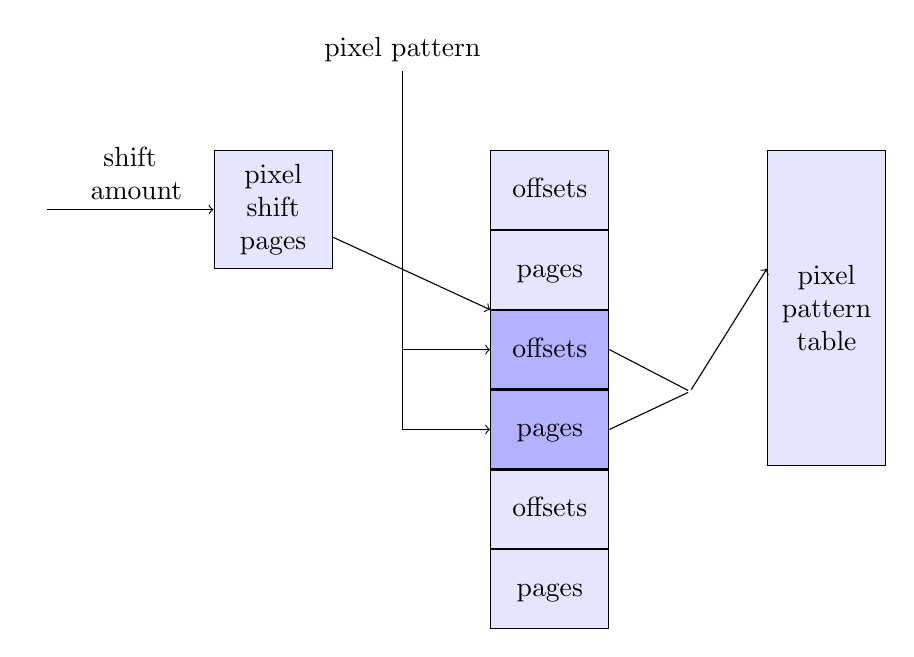
\begin{tikzpicture}
  [basicbox/.style={draw,rectangle,inner sep=0pt,minimum width=1.5cm,minimum height=1.5cm,fill=blue!10},
   pageoffsets/.style={basicbox,minimum height=1cm,text height=1.5ex,text depth=.25ex},
   multilinebox/.style={basicbox,text width=1cm,align=center}]
  \node (pixelshiftpages) at (0,0) [multilinebox] {pixel shift pages};
  \node (start) at (-3,0) {};
  \draw [->] (start) -- (pixelshiftpages) node [above,text width=1cm,align=center,midway] {shift amount};
  \node (offsets0) [pageoffsets,anchor=north,below right=0 and 2 of pixelshiftpages.north east] {offsets};
  \node (pages0) [pageoffsets,below=0 of offsets0.south] {pages};
  \node (offsets1) [pageoffsets,below=0 of pages0.south,fill=blue!30] {offsets};
  \node (pages1) [pageoffsets,below=0 of offsets1.south,fill=blue!30] {pages};
  \node (offsets2) [pageoffsets,below=0 of pages1.south] {offsets};
  \node (pages2) [pageoffsets,below=0 of offsets2.south] {pages};
  \draw [->] (pixelshiftpages) -- (offsets1.north west) {};
  \node (pixelpattern) [above left=1 and 0 of offsets0.north west] {pixel pattern};
  \draw [->] (pixelpattern.south) |- (offsets1.west) {};
  \draw [->] (pixelpattern.south) |- (pages1.west) {};
  \node (patterntable) [multilinebox,minimum height=4cm,text width=1.2cm,anchor=north west,below right=0 and 2 of offsets0.north east] {pixel pattern table};
  \node (join) [inner sep=0pt,below right=0 and 1 of offsets1.south east] {};
  \draw (offsets1.east) -- (join);
  \draw (pages1.east) -- (join);
  \draw [->] (join) -- ([yshift=5mm]patterntable.west);
\end{tikzpicture}
\vspace{1em}

The pixel pattern table is a table of every possible pattern of 7 consecutive pixels
spread out over two bytes. This table is 512 entries, each entry being two bytes.
A naive table would have redundancy. For example the pattern {\Tt{}0000100\nwendquote} starting
at column 0 is exactly the same as the pattern {\Tt{}0001000\nwendquote} starting at column 1.
This table eliminates that redundancy.

\nwenddocs{}\nwbegincode{8}\sublabel{NW1Xx3lK-1W8AJS-2}\nwmargintag{{\nwtagstyle{}\subpageref{NW1Xx3lK-1W8AJS-2}}}\moddef{tables~{\nwtagstyle{}\subpageref{NW1Xx3lK-1W8AJS-1}}}\plusendmoddef\nwstartdeflinemarkup\nwprevnextdefs{NW1Xx3lK-1W8AJS-1}{NW1Xx3lK-1W8AJS-3}\nwenddeflinemarkup
    ORG     $A900
\nwlinkedidentc{PIXEL_PATTERN_TABLE}{NW1Xx3lK-1W8AJS-2}:
    INCLUDE "pixel_pattern_table.asm"
\nwindexdefn{\nwixident{PIXEL{\_}PATTERN{\_}TABLE}}{PIXEL:unPATTERN:unTABLE}{NW1Xx3lK-1W8AJS-2}\eatline
\nwidentdefs{\\{{\nwixident{PIXEL{\_}PATTERN{\_}TABLE}}{PIXEL:unPATTERN:unTABLE}}}\nwendcode{}\nwbegindocs{9}\nwdocspar
Now we just need tables which index into {\Tt{}\nwlinkedidentq{PIXEL{\_}PATTERN{\_}TABLE}{NW1Xx3lK-1W8AJS-2}\nwendquote} for every
7-pixel pattern and shift value. This table works by having the page number
for the shifted pixel pattern at index {\Tt{}shift\ *\ 0x100\ +\ 0x80\ +\ pattern\nwendquote}
and the offset at index {\Tt{}shift\ *\ 0x100\ +\ pattern\nwendquote}.

\nwenddocs{}\nwbegincode{10}\sublabel{NW1Xx3lK-1W8AJS-3}\nwmargintag{{\nwtagstyle{}\subpageref{NW1Xx3lK-1W8AJS-3}}}\moddef{tables~{\nwtagstyle{}\subpageref{NW1Xx3lK-1W8AJS-1}}}\plusendmoddef\nwstartdeflinemarkup\nwprevnextdefs{NW1Xx3lK-1W8AJS-2}{NW1Xx3lK-1W8AJS-4}\nwenddeflinemarkup
    ORG     $A200
\nwlinkedidentc{PIXEL_SHIFT_TABLE}{NW1Xx3lK-1W8AJS-3}:
    INCLUDE "pixel_shift_table.asm"
\nwindexdefn{\nwixident{PIXEL{\_}SHIFT{\_}TABLE}}{PIXEL:unSHIFT:unTABLE}{NW1Xx3lK-1W8AJS-3}\eatline
\nwidentdefs{\\{{\nwixident{PIXEL{\_}SHIFT{\_}TABLE}}{PIXEL:unSHIFT:unTABLE}}}\nwendcode{}\nwbegindocs{11}\nwdocspar
Rather than multiplying the shift value by {\Tt{}0x100\nwendquote}, we instead define
another table which holds the page numbers for the shift tables for each
shift value.

\nwenddocs{}\nwbegincode{12}\sublabel{NW1Xx3lK-1W8AJS-4}\nwmargintag{{\nwtagstyle{}\subpageref{NW1Xx3lK-1W8AJS-4}}}\moddef{tables~{\nwtagstyle{}\subpageref{NW1Xx3lK-1W8AJS-1}}}\plusendmoddef\nwstartdeflinemarkup\nwprevnextdefs{NW1Xx3lK-1W8AJS-3}{NW1Xx3lK-1W8AJS-5}\nwenddeflinemarkup
    ORG     $84C1
\nwlinkedidentc{PIXEL_SHIFT_PAGES}{NW1Xx3lK-1W8AJS-4}:
    HEX     A2 A3 A4 A5 A6 A7 A8
\nwindexdefn{\nwixident{PIXEL{\_}SHIFT{\_}PAGES}}{PIXEL:unSHIFT:unPAGES}{NW1Xx3lK-1W8AJS-4}\eatline
\nwidentdefs{\\{{\nwixident{PIXEL{\_}SHIFT{\_}PAGES}}{PIXEL:unSHIFT:unPAGES}}}\nwendcode{}\nwbegindocs{13}\nwdocspar
So we can get shifted pixels by indexing into all these tables.

Now we can define a routine that will take a sprite number and a pixel shift
amount, and write the shifted pixel data into the {\Tt{}\nwlinkedidentq{BLOCK{\_}DATA}{NW1Xx3lK-10jlgu-1}\nwendquote} area. The
routine first shifts the first byte of the sprite into a two-byte area. Then
it shifts the second byte of the sprite, and combines that two-byte result
with the first. Thus, we shift two bytes of sprite data into a three-byte
result.

\begin{center}
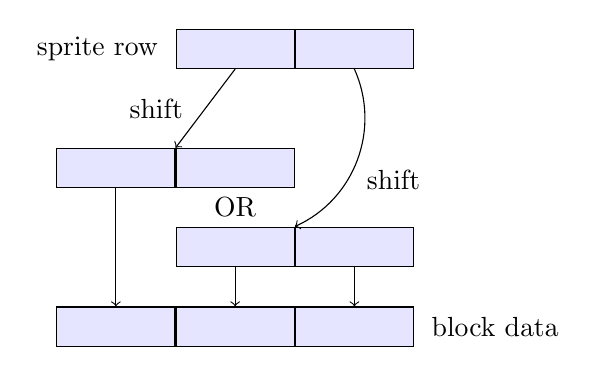
\begin{tikzpicture}
  [basicbox/.style={draw,rectangle,inner sep=0pt,minimum width=1.5cm,minimum height=0.5cm,fill=blue!10}]
  \node (spriterowbyte0) at (0,0) [basicbox] {};
  \node (spriterowbyte1) [basicbox,right=0 of spriterowbyte0.east] {};
  \node (spriterowlabel) [left=0.1 of spriterowbyte0.west] {sprite row};
  \node (shifted0byte0) [basicbox,below left=1 and 0 of spriterowbyte0.south west] {};
  \node (shifted0byte1) [basicbox,right=0 of shifted0byte0.east] {};
  \node (shifted1byte0) [basicbox,below right=2 and 0 of spriterowbyte0.south west] {};
  \node (shifted1byte1) [basicbox,right=0 of shifted1byte0.east] {};
  \node (orlabel) [below=0 of shifted0byte1] {OR};
  \draw [->] (spriterowbyte0.south) -- (shifted0byte0.north east)
    node [left,text width=1cm,align=center,midway] {shift};
  \draw [->] (spriterowbyte1.south) to [auto, bend left=45] node {shift} (shifted1byte0.north east);
  \node (result0) [basicbox,below left=0.5 and 0 of shifted1byte0.south west] {};
  \node (result1) [basicbox,right=0 of result0.east] {};
  \node (result2) [basicbox,right=0 of result1.east] {};
  \draw [->] (shifted0byte0) -- (result0) {};
  \draw [->] (shifted1byte0) -- (result1) {};
  \draw [->] (shifted1byte1) -- (result2) {};
  \node (blocklabel) [right=0.1 of result2.east] {block data};
\end{tikzpicture}
\end{center}

Rather than load addresses from the tables and store them, the routine
modifies its own instructions with those addresses.

\nwenddocs{}\nwbegincode{14}\sublabel{NW1Xx3lK-10jlgu-2}\nwmargintag{{\nwtagstyle{}\subpageref{NW1Xx3lK-10jlgu-2}}}\moddef{defines~{\nwtagstyle{}\subpageref{NW1Xx3lK-10jlgu-1}}}\plusendmoddef\nwstartdeflinemarkup\nwprevnextdefs{NW1Xx3lK-10jlgu-1}{NW1Xx3lK-10jlgu-3}\nwenddeflinemarkup
    ORG     $0A
\nwlinkedidentc{TMP_PTR}{NW1Xx3lK-10jlgu-2}         DS.W    1
    ORG     $1D
\nwlinkedidentc{ROW_COUNT}{NW1Xx3lK-10jlgu-2}       DS      1
\nwlinkedidentc{SPRITE_NUM}{NW1Xx3lK-10jlgu-2}      DS      1
\nwindexdefn{\nwixident{TMP{\_}PTR}}{TMP:unPTR}{NW1Xx3lK-10jlgu-2}\nwindexdefn{\nwixident{ROW{\_}COUNT}}{ROW:unCOUNT}{NW1Xx3lK-10jlgu-2}\nwindexdefn{\nwixident{SPRITE{\_}NUM}}{SPRITE:unNUM}{NW1Xx3lK-10jlgu-2}\eatline
\nwidentdefs{\\{{\nwixident{ROW{\_}COUNT}}{ROW:unCOUNT}}\\{{\nwixident{SPRITE{\_}NUM}}{SPRITE:unNUM}}\\{{\nwixident{TMP{\_}PTR}}{TMP:unPTR}}}\nwendcode{}\nwbegindocs{15}\nwdocspar
\nwenddocs{}\nwbegincode{16}\sublabel{NW1Xx3lK-8jv1b-1}\nwmargintag{{\nwtagstyle{}\subpageref{NW1Xx3lK-8jv1b-1}}}\moddef{routines~{\nwtagstyle{}\subpageref{NW1Xx3lK-8jv1b-1}}}\endmoddef\nwstartdeflinemarkup\nwprevnextdefs{\relax}{NW1Xx3lK-8jv1b-2}\nwenddeflinemarkup
    ORG     $8438
\nwlinkedidentc{COMPUTE_SHIFTED_SPRITE}{NW1Xx3lK-8jv1b-1}:
    SUBROUTINE
    ; Enter routine with X set to pixel shift amount and
    ; \nwlinkedidentc{SPRITE_NUM}{NW1Xx3lK-10jlgu-2} containing the sprite number to read.

.offset_table       EQU $A000               ; Target addresses in read
.page_table         EQU $A080               ; instructions. The only truly
.shift_ptr_byte0    EQU $A000               ; necessary value here is the
.shift_ptr_byte1    EQU $A000               ; 0x80 in .shift_ptr_byte0.

    LDA     #$0B                            ; 11 rows
    STA     \nwlinkedidentc{ROW_COUNT}{NW1Xx3lK-10jlgu-2}
    LDA     #<\nwlinkedidentc{SPRITE_DATA}{NW1Xx3lK-1W8AJS-1}
    STA     \nwlinkedidentc{TMP_PTR}{NW1Xx3lK-10jlgu-2}
    LDA     #>\nwlinkedidentc{SPRITE_DATA}{NW1Xx3lK-1W8AJS-1}
    STA     \nwlinkedidentc{TMP_PTR}{NW1Xx3lK-10jlgu-2}+1                       ; \nwlinkedidentc{TMP_PTR}{NW1Xx3lK-10jlgu-2} = \nwlinkedidentc{SPRITE_DATA}{NW1Xx3lK-1W8AJS-1}
    LDA     \nwlinkedidentc{PIXEL_SHIFT_PAGES}{NW1Xx3lK-1W8AJS-4}, X
    STA     .rd_offset_table + 2
    STA     .rd_page_table + 2
    STA     .rd_offset_table2 + 2
    STA     .rd_page_table2 + 2             ; Fix up pages in lookup instructions
                                            ; based on shift amount (X).

    LDX     #$00                            ; X is the offset into \nwlinkedidentc{BLOCK_DATA}{NW1Xx3lK-10jlgu-1}.

.loop:                                      ; === LOOP === (over all 11 rows)
    LDY     \nwlinkedidentc{SPRITE_NUM}{NW1Xx3lK-10jlgu-2}
    LDA     (\nwlinkedidentc{TMP_PTR}{NW1Xx3lK-10jlgu-2}), Y
    TAY                                     ; Get sprite pixel data.

.rd_offset_table:
    LDA     .offset_table, Y                ; Load offset for shift amount.
    STA     .rd_shift_ptr_byte0 + 1
    CLC
    ADC     #$01
    STA     .rd_shift_ptr_byte1 + 1         ; Fix up instruction offsets with it.
.rd_page_table:
    LDA     .page_table, Y                  ; Load page for shift amount.
    STA     .rd_shift_ptr_byte0 + 2
    STA     .rd_shift_ptr_byte1 + 2         ; Fix up instruction page with it.

.rd_shift_ptr_byte0:
    LDA     .shift_ptr_byte0                ; Read shifted pixel data byte 0
    STA     \nwlinkedidentc{BLOCK_DATA}{NW1Xx3lK-10jlgu-1}, X                   ; and store in block data byte 0.
.rd_shift_ptr_byte1:
    LDA     .shift_ptr_byte1                ; Read shifted pixel data byte 1
    STA     \nwlinkedidentc{BLOCK_DATA}{NW1Xx3lK-10jlgu-1}+1, X                 ; and store in block data byte 1.

    LDA     \nwlinkedidentc{TMP_PTR}{NW1Xx3lK-10jlgu-2}
    CLC
    ADC     #$68
    STA     \nwlinkedidentc{TMP_PTR}{NW1Xx3lK-10jlgu-2}
    LDA     \nwlinkedidentc{TMP_PTR}{NW1Xx3lK-10jlgu-2}+1
    ADC     #$00
    STA     \nwlinkedidentc{TMP_PTR}{NW1Xx3lK-10jlgu-2}+1                       ; \nwlinkedidentc{TMP_PTR}{NW1Xx3lK-10jlgu-2}++

    ; Now basically do the same thing with the second sprite byte

    LDY     \nwlinkedidentc{SPRITE_NUM}{NW1Xx3lK-10jlgu-2}
    LDA     (\nwlinkedidentc{TMP_PTR}{NW1Xx3lK-10jlgu-2}), Y
    TAY                                     ; Get sprite pixel data.

.rd_offset_table2:
    LDA     .offset_table, Y                ; Load offset for shift amount.
    STA     .rd_shift_ptr2_byte0 + 1
    CLC
    ADC     #$01
    STA     .rd_shift_ptr2_byte1 + 1        ; Fix up instruction offsets with it.
.rd_page_table2:
    LDA     .page_table, Y                  ; Load page for shift amount.
    STA     .rd_shift_ptr2_byte0 + 2
    STA     .rd_shift_ptr2_byte1 + 2        ; Fix up instruction page with it.

.rd_shift_ptr2_byte0:
    LDA     .shift_ptr_byte0                ; Read shifted pixel data byte 0
    ORA     \nwlinkedidentc{BLOCK_DATA}{NW1Xx3lK-10jlgu-1}+1, X                 ; OR with previous block data byte 1
    STA     \nwlinkedidentc{BLOCK_DATA}{NW1Xx3lK-10jlgu-1}+1, X                 ; and store in block data byte 1.
.rd_shift_ptr2_byte1:
    LDA     .shift_ptr_byte1                ; Read shifted pixel data byte 1
    STA     \nwlinkedidentc{BLOCK_DATA}{NW1Xx3lK-10jlgu-1}+2, X                 ; and store in block data byte 2.

    LDA     \nwlinkedidentc{TMP_PTR}{NW1Xx3lK-10jlgu-2}
    CLC
    ADC     #$68
    STA     \nwlinkedidentc{TMP_PTR}{NW1Xx3lK-10jlgu-2}
    LDA     \nwlinkedidentc{TMP_PTR}{NW1Xx3lK-10jlgu-2}+1
    ADC     #$00
    STA     \nwlinkedidentc{TMP_PTR}{NW1Xx3lK-10jlgu-2}+1                       ; \nwlinkedidentc{TMP_PTR}{NW1Xx3lK-10jlgu-2}++

    INX
    INX
    INX                                     ; X += 3
    DEC     \nwlinkedidentc{ROW_COUNT}{NW1Xx3lK-10jlgu-2}                       ; \nwlinkedidentc{ROW_COUNT}{NW1Xx3lK-10jlgu-2}--
    BNE     .loop                           ; loop while \nwlinkedidentc{ROW_COUNT}{NW1Xx3lK-10jlgu-2} > 0
    RTS
\nwindexdefn{\nwixident{COMPUTE{\_}SHIFTED{\_}SPRITE}}{COMPUTE:unSHIFTED:unSPRITE}{NW1Xx3lK-8jv1b-1}\eatline
\nwalsodefined{\\{NW1Xx3lK-8jv1b-2}\\{NW1Xx3lK-8jv1b-3}}\nwnotused{routines}\nwidentdefs{\\{{\nwixident{COMPUTE{\_}SHIFTED{\_}SPRITE}}{COMPUTE:unSHIFTED:unSPRITE}}}\nwidentuses{\\{{\nwixident{BLOCK{\_}DATA}}{BLOCK:unDATA}}\\{{\nwixident{PIXEL{\_}SHIFT{\_}PAGES}}{PIXEL:unSHIFT:unPAGES}}\\{{\nwixident{ROW{\_}COUNT}}{ROW:unCOUNT}}\\{{\nwixident{SPRITE{\_}DATA}}{SPRITE:unDATA}}\\{{\nwixident{SPRITE{\_}NUM}}{SPRITE:unNUM}}\\{{\nwixident{TMP{\_}PTR}}{TMP:unPTR}}}\nwindexuse{\nwixident{BLOCK{\_}DATA}}{BLOCK:unDATA}{NW1Xx3lK-8jv1b-1}\nwindexuse{\nwixident{PIXEL{\_}SHIFT{\_}PAGES}}{PIXEL:unSHIFT:unPAGES}{NW1Xx3lK-8jv1b-1}\nwindexuse{\nwixident{ROW{\_}COUNT}}{ROW:unCOUNT}{NW1Xx3lK-8jv1b-1}\nwindexuse{\nwixident{SPRITE{\_}DATA}}{SPRITE:unDATA}{NW1Xx3lK-8jv1b-1}\nwindexuse{\nwixident{SPRITE{\_}NUM}}{SPRITE:unNUM}{NW1Xx3lK-8jv1b-1}\nwindexuse{\nwixident{TMP{\_}PTR}}{TMP:unPTR}{NW1Xx3lK-8jv1b-1}\nwendcode{}\nwbegindocs{17}\nwdocspar
\section{Memory mapped graphics}

The Apple II maps the area from {\Tt{}{\$}2000-{\$}3FFF\nwendquote} to high-res graphics page 1 (HGR1),
and {\Tt{}{\$}4000-{\$}5FFF\nwendquote} to page 2 (HGR2). Within a row, consecutive bytes map to
consecutive pixels. However, rows themselves are not consecutive in memory.

To make it easy to convert a row number from 0 to 191 to a base address, Lode Runner has
a table and a routine to use that table.

\nwenddocs{}\nwbegincode{18}\sublabel{NW1Xx3lK-1W8AJS-5}\nwmargintag{{\nwtagstyle{}\subpageref{NW1Xx3lK-1W8AJS-5}}}\moddef{tables~{\nwtagstyle{}\subpageref{NW1Xx3lK-1W8AJS-1}}}\plusendmoddef\nwstartdeflinemarkup\nwprevnextdefs{NW1Xx3lK-1W8AJS-4}{NW1Xx3lK-1W8AJS-6}\nwenddeflinemarkup
    ORG     $1A85
\nwlinkedidentc{ROW_TO_OFFSET_LO}{NW1Xx3lK-1W8AJS-5}:
    INCLUDE "row_to_offset_lo_table.asm"
\nwlinkedidentc{ROW_TO_OFFSET_HI}{NW1Xx3lK-1W8AJS-5}:
    INCLUDE "row_to_offset_hi_table.asm"
\nwindexdefn{\nwixident{ROW{\_}TO{\_}OFFSET{\_}LO}}{ROW:unTO:unOFFSET:unLO}{NW1Xx3lK-1W8AJS-5}\nwindexdefn{\nwixident{ROW{\_}TO{\_}OFFSET{\_}HI}}{ROW:unTO:unOFFSET:unHI}{NW1Xx3lK-1W8AJS-5}\eatline
\nwidentdefs{\\{{\nwixident{ROW{\_}TO{\_}OFFSET{\_}HI}}{ROW:unTO:unOFFSET:unHI}}\\{{\nwixident{ROW{\_}TO{\_}OFFSET{\_}LO}}{ROW:unTO:unOFFSET:unLO}}}\nwendcode{}\nwbegindocs{19}\nwdocspar
\nwenddocs{}\nwbegincode{20}\sublabel{NW1Xx3lK-10jlgu-3}\nwmargintag{{\nwtagstyle{}\subpageref{NW1Xx3lK-10jlgu-3}}}\moddef{defines~{\nwtagstyle{}\subpageref{NW1Xx3lK-10jlgu-1}}}\plusendmoddef\nwstartdeflinemarkup\nwprevnextdefs{NW1Xx3lK-10jlgu-2}{\relax}\nwenddeflinemarkup
    ORG     $0C
\nwlinkedidentc{ROW_ADDR}{NW1Xx3lK-10jlgu-3}    DS      2
    ORG     $1F
\nwlinkedidentc{HGR_PAGE}{NW1Xx3lK-10jlgu-3}    DS      1       ; 0x20 for HGR1, 0x40 for HGR2
\nwindexdefn{\nwixident{ROW{\_}ADDR}}{ROW:unADDR}{NW1Xx3lK-10jlgu-3}\nwindexdefn{\nwixident{HGR{\_}PAGE}}{HGR:unPAGE}{NW1Xx3lK-10jlgu-3}\eatline
\nwidentdefs{\\{{\nwixident{HGR{\_}PAGE}}{HGR:unPAGE}}\\{{\nwixident{ROW{\_}ADDR}}{ROW:unADDR}}}\nwendcode{}\nwbegindocs{21}\nwdocspar
\nwenddocs{}\nwbegincode{22}\sublabel{NW1Xx3lK-8jv1b-2}\nwmargintag{{\nwtagstyle{}\subpageref{NW1Xx3lK-8jv1b-2}}}\moddef{routines~{\nwtagstyle{}\subpageref{NW1Xx3lK-8jv1b-1}}}\plusendmoddef\nwstartdeflinemarkup\nwprevnextdefs{NW1Xx3lK-8jv1b-1}{NW1Xx3lK-8jv1b-3}\nwenddeflinemarkup
    ORG     $7A31
\nwlinkedidentc{ROW_TO_ADDR}{NW1Xx3lK-8jv1b-2}:
    SUBROUTINE
    ; Enter routine with Y set to row. Base address
    ; (for column 0) will be placed in \nwlinkedidentc{ROW_ADDR}{NW1Xx3lK-10jlgu-3}.

    LDA     \nwlinkedidentc{ROW_TO_OFFSET_LO}{NW1Xx3lK-1W8AJS-5}, Y
    STA     \nwlinkedidentc{ROW_ADDR}{NW1Xx3lK-10jlgu-3}
    LDA     \nwlinkedidentc{ROW_TO_OFFSET_HI}{NW1Xx3lK-1W8AJS-5}, Y
    ORA     \nwlinkedidentc{HGR_PAGE}{NW1Xx3lK-10jlgu-3}
    STA     \nwlinkedidentc{ROW_ADDR}{NW1Xx3lK-10jlgu-3}+1
    RTS
\nwindexdefn{\nwixident{ROW{\_}TO{\_}ADDR}}{ROW:unTO:unADDR}{NW1Xx3lK-8jv1b-2}\eatline
\nwidentdefs{\\{{\nwixident{ROW{\_}TO{\_}ADDR}}{ROW:unTO:unADDR}}}\nwidentuses{\\{{\nwixident{HGR{\_}PAGE}}{HGR:unPAGE}}\\{{\nwixident{ROW{\_}ADDR}}{ROW:unADDR}}\\{{\nwixident{ROW{\_}TO{\_}OFFSET{\_}HI}}{ROW:unTO:unOFFSET:unHI}}\\{{\nwixident{ROW{\_}TO{\_}OFFSET{\_}LO}}{ROW:unTO:unOFFSET:unLO}}}\nwindexuse{\nwixident{HGR{\_}PAGE}}{HGR:unPAGE}{NW1Xx3lK-8jv1b-2}\nwindexuse{\nwixident{ROW{\_}ADDR}}{ROW:unADDR}{NW1Xx3lK-8jv1b-2}\nwindexuse{\nwixident{ROW{\_}TO{\_}OFFSET{\_}HI}}{ROW:unTO:unOFFSET:unHI}{NW1Xx3lK-8jv1b-2}\nwindexuse{\nwixident{ROW{\_}TO{\_}OFFSET{\_}LO}}{ROW:unTO:unOFFSET:unLO}{NW1Xx3lK-8jv1b-2}\nwendcode{}\nwbegindocs{23}\nwdocspar
Lode Runner's screens are organized into 28 sprites across by 17 sprites
down. To convert between sprite coordinates and screen coordinates, we
use tables and lookup routines.

\nwenddocs{}\nwbegincode{24}\sublabel{NW1Xx3lK-1W8AJS-6}\nwmargintag{{\nwtagstyle{}\subpageref{NW1Xx3lK-1W8AJS-6}}}\moddef{tables~{\nwtagstyle{}\subpageref{NW1Xx3lK-1W8AJS-1}}}\plusendmoddef\nwstartdeflinemarkup\nwprevnextdefs{NW1Xx3lK-1W8AJS-5}{\relax}\nwenddeflinemarkup
    ORG     $1C51
\nwlinkedidentc{ROW_TABLE}{NW1Xx3lK-1W8AJS-6}:
    HEX     00 0B 16 21 2C 37 42 4D
    HEX     58 63 6E 79 84 8F 9A A5
    HEX     B5
\nwlinkedidentc{COL_TABLE}{NW1Xx3lK-1W8AJS-6}:
    HEX     00 01 02 04 05 07 08 0A
    HEX     0B 0C 0E 0F 11 12 14 15
    HEX     16 18 19 1B 1C 1E 1F 20
    HEX     22 23 25 26
\nwindexdefn{\nwixident{ROW{\_}TABLE}}{ROW:unTABLE}{NW1Xx3lK-1W8AJS-6}\nwindexdefn{\nwixident{COL{\_}TABLE}}{COL:unTABLE}{NW1Xx3lK-1W8AJS-6}\eatline
\nwidentdefs{\\{{\nwixident{COL{\_}TABLE}}{COL:unTABLE}}\\{{\nwixident{ROW{\_}TABLE}}{ROW:unTABLE}}}\nwendcode{}\nwbegindocs{25}\nwdocspar
\nwenddocs{}\nwbegincode{26}\sublabel{NW1Xx3lK-8jv1b-3}\nwmargintag{{\nwtagstyle{}\subpageref{NW1Xx3lK-8jv1b-3}}}\moddef{routines~{\nwtagstyle{}\subpageref{NW1Xx3lK-8jv1b-1}}}\plusendmoddef\nwstartdeflinemarkup\nwprevnextdefs{NW1Xx3lK-8jv1b-2}{\relax}\nwenddeflinemarkup
    ORG     $885D
GET_ROWNUM_FOR:
    SUBROUTINE
    ; Enter routine with Y set to sprite row. On
    ; return, Y will be set to screen row.

    LDA     \nwlinkedidentc{ROW_TABLE}{NW1Xx3lK-1W8AJS-6}, Y
    PHA
    LDA     

\\chapter\{The whole thing\}
We then put together the entire assembly file:

\nwidentuses{\\{{\nwixident{ROW{\_}TABLE}}{ROW:unTABLE}}}\nwindexuse{\nwixident{ROW{\_}TABLE}}{ROW:unTABLE}{NW1Xx3lK-8jv1b-3}\nwendcode{}\nwbegincode{27}\sublabel{NW1Xx3lK-1p0Y9w-1}\nwmargintag{{\nwtagstyle{}\subpageref{NW1Xx3lK-1p0Y9w-1}}}\moddef{*~{\nwtagstyle{}\subpageref{NW1Xx3lK-1p0Y9w-1}}}\endmoddef\nwstartdeflinemarkup\nwenddeflinemarkup
\LA{}preamble~{\nwtagstyle{}\subpageref{NW1Xx3lK-1jwKhK-1}}\RA{}
\LA{}row mapping~{\nwtagstyle{}\subpageref{nw@notdef}}\RA{}
\nwnotused{*}\nwendcode{}\nwbegindocs{28}\nwdocspar

\chapter{Defined Chunks}\par\noindent
\nowebchunks
\chapter{Index}\par\noindent
\nowebindex
\nwenddocs{}

\nwixlogsorted{c}{{*}{NW1Xx3lK-1p0Y9w-1}{\nwixd{NW1Xx3lK-1p0Y9w-1}}}%
\nwixlogsorted{c}{{defines}{NW1Xx3lK-10jlgu-1}{\nwixd{NW1Xx3lK-10jlgu-1}\nwixd{NW1Xx3lK-10jlgu-2}\nwixd{NW1Xx3lK-10jlgu-3}}}%
\nwixlogsorted{c}{{preamble}{NW1Xx3lK-1jwKhK-1}{\nwixd{NW1Xx3lK-1jwKhK-1}\nwixu{NW1Xx3lK-1p0Y9w-1}}}%
\nwixlogsorted{c}{{routines}{NW1Xx3lK-8jv1b-1}{\nwixd{NW1Xx3lK-8jv1b-1}\nwixd{NW1Xx3lK-8jv1b-2}\nwixd{NW1Xx3lK-8jv1b-3}}}%
\nwixlogsorted{c}{{row mapping}{nw@notdef}{\nwixu{NW1Xx3lK-1p0Y9w-1}}}%
\nwixlogsorted{c}{{tables}{NW1Xx3lK-1W8AJS-1}{\nwixd{NW1Xx3lK-1W8AJS-1}\nwixd{NW1Xx3lK-1W8AJS-2}\nwixd{NW1Xx3lK-1W8AJS-3}\nwixd{NW1Xx3lK-1W8AJS-4}\nwixd{NW1Xx3lK-1W8AJS-5}\nwixd{NW1Xx3lK-1W8AJS-6}}}%
\nwixlogsorted{i}{{\nwixident{BLOCK{\_}DATA}}{BLOCK:unDATA}}%
\nwixlogsorted{i}{{\nwixident{COL{\_}TABLE}}{COL:unTABLE}}%
\nwixlogsorted{i}{{\nwixident{COMPUTE{\_}SHIFTED{\_}SPRITE}}{COMPUTE:unSHIFTED:unSPRITE}}%
\nwixlogsorted{i}{{\nwixident{HGR{\_}PAGE}}{HGR:unPAGE}}%
\nwixlogsorted{i}{{\nwixident{PIXEL{\_}PATTERN{\_}TABLE}}{PIXEL:unPATTERN:unTABLE}}%
\nwixlogsorted{i}{{\nwixident{PIXEL{\_}SHIFT{\_}PAGES}}{PIXEL:unSHIFT:unPAGES}}%
\nwixlogsorted{i}{{\nwixident{PIXEL{\_}SHIFT{\_}TABLE}}{PIXEL:unSHIFT:unTABLE}}%
\nwixlogsorted{i}{{\nwixident{ROW{\_}ADDR}}{ROW:unADDR}}%
\nwixlogsorted{i}{{\nwixident{ROW{\_}COUNT}}{ROW:unCOUNT}}%
\nwixlogsorted{i}{{\nwixident{ROW{\_}TABLE}}{ROW:unTABLE}}%
\nwixlogsorted{i}{{\nwixident{ROW{\_}TO{\_}ADDR}}{ROW:unTO:unADDR}}%
\nwixlogsorted{i}{{\nwixident{ROW{\_}TO{\_}OFFSET{\_}HI}}{ROW:unTO:unOFFSET:unHI}}%
\nwixlogsorted{i}{{\nwixident{ROW{\_}TO{\_}OFFSET{\_}LO}}{ROW:unTO:unOFFSET:unLO}}%
\nwixlogsorted{i}{{\nwixident{SPRITE{\_}DATA}}{SPRITE:unDATA}}%
\nwixlogsorted{i}{{\nwixident{SPRITE{\_}NUM}}{SPRITE:unNUM}}%
\nwixlogsorted{i}{{\nwixident{TMP{\_}PTR}}{TMP:unPTR}}%
\nwbegindocs{29}\nwdocspar
\end{document}
\nwenddocs{}
